% Core.Tex, version=13
% Satin Dmitri, 2016-2018

% Changelog:
% 13: Add No Title mode
% 12.1: Improve \N, \Q, \R, \Z, \CC definitions a bit, add some customizations for moth mode
% 12: Improve \TODO, \skip[sub][sub]section (takes optional counter now), fix code a bit, add exec end.
% 11: Add cmap
% 10.6: Styling changes
% 10.5: Add \slashn stuff, custom theorem namespace support, style changes.
% 10.4: replace \emptyset in math mode.
% 10.3: add properties(theorems), add \ref example, add \ThmSpacing configure var.
% 10.2: fix for proofs
% 10.1: better style for theorems, thmslashn
% 10: more math symbols, theorems support (\enablemath), using paralist, using cancel, moved code support to \enablecode
% 9: new math symbols (\enablemath), \skip[sub][sub]section, \CustomTitle support
% 8: better source code support, padding.
% 7: custom head, foot, sections.

\documentclass[a4paper,12pt]{article}
%\usepackage{cmap}
\usepackage[usenames,dvipsnames]{xcolor}
\usepackage{polyglossia}
\usepackage{xspace}
\usepackage{mathrsfs}
\setdefaultlanguage[spelling=modern]{russian}
\setotherlanguage{english}
\defaultfontfeatures{Ligatures={TeX},Renderer=Basic}
\setmainfont[Ligatures={TeX,Historic}]{CMU Serif}
\newfontfamily{\cyrillicfont}{CMU Serif}
\setsansfont{CMU Sans Serif}
\newfontfamily{\cyrillicfontsf}{CMU Sans Serif}
\setmonofont{CMU Typewriter Text}
\newfontfamily{\cyrillicfonttt}{CMU Typewriter Text}
\let\CYRDZE\relax
\usepackage{graphicx}

\pagestyle{plain}
\usepackage[
  left=0.50in,
  right=0.50in,
  top=0.8in,
  bottom=0.7in,
  headheight=0.8in]{geometry}
\pagenumbering{gobble}

\setlength{\parskip}{0.15cm}

\usepackage{indentfirst}

\usepackage{hyperref}
\hypersetup{
  colorlinks,
  citecolor=black,
  filecolor=black,
  linkcolor=blue,
  urlcolor=blue
}

\usepackage{paralist}
\usepackage{cancel}
\usepackage{textcomp}
\usepackage{gensymb}
\usepackage{mdframed}
\usepackage{lastpage}
\usepackage{microtype}
\usepackage[super]{cite}
\usepackage{fancyhdr}
\pagestyle{fancy}

% Основано на коде С. Копелиовича.
\newcommand\Section[2]{
  \newpage % new page
  \stepcounter{section}
  \bigskip
  \phantomsection
  \addcontentsline{toc}{section}{\arabic{section}. #1}
  \begin{center}
    {\huge \bf \arabic{section}. #1}\\
  \end{center}
  \bigskip
  \gdef\SectionName{#1}
  \gdef\AuthorName{#2}

  \lhead{\ShortCourseName}
  \chead{}
  \rhead{\SectionName}

  \cfoot{
%    \topskip0pt\vspace*{\fill}
    \thepage~из~\pageref*{LastPage}
%    \vspace*{\fill}
  }
  
  \renewcommand{\headrulewidth}{0.15 mm}

  \ifx\LaconicFooter\undefined
  \lfoot{
%    \topskip0pt\vspace*{\fill}
    Глава \texttt{\#\arabic{section}}
%    \vspace*{\fill}
  }
  \rfoot{
%    \topskip0pt\vspace*{\fill}
    Автор: \AuthorName
%    \vspace*{\fill}
  }
  \renewcommand{\footrulewidth}{0.15 mm}
  \fi
}

\newcommand\Subsection[1]{
  % Пока здесь нет никаких кастомизаций,
  % Но рекомендуется использовать имено вариацию с большой буквы,
  % На случай, если в будущем они появятся.
  \subsection{#1}
}

\newcommand\Subsubsection[1]{
  % Пока здесь нет никаких кастомизаций,
  % Но рекомендуется использовать имено вариацию с большой буквы,
  % На случай, если в будущем они появятся.
  \subsubsection{#1}
}

\newcommand\slashnl{~\\*[-26pt]}
\newcommand\slashn{~\\*[-22pt]}
\newcommand\slashns{~\\*[-18pt]}
\newcommand\slashnss{~\\*[-14pt]}
\newcommand\slashnsss{~\\*[-10pt]}

\newcommand{\makegood}{
  \ifx\ShortCourseName\undefined
  \gdef\ShortCourseName{\CourseName}
  \fi
  
  % \new command\Custom Title{...} до \make good для того, чтобы
  % переопределить содержимое титульной страницы до содержания.

  \ifx\NoTitlePage\undefined
  
  \ifx\CustomTitle\undefined
    \title{\CourseName}
    \maketitle
  \else
    \pagestyle{empty}
    \CustomTitle
  \fi
  \tableofcontents
  \pagebreak
  \fi
  
  \pagestyle{fancy}
  \pagenumbering{arabic}
  \setcounter{page}{1}

  \lhead{\ShortCourseName}
  
  \ifdefined\ENABLEDMATH
  \renewcommand\proofname{\em\textbf{Доказательство}}
  \else
  \fi
}

% Использовать как \skipsection или \skipsection[2]

\newcommand\skipsection[1][1]{
  \addtocounter{section}{#1}
}

\newcommand\skipsubsection[1][1]{
  \addtocounter{subsection}{#1}
}

\newcommand\skipsubsubsection[1][1]{
  \addtocounter{subsubsection}{#1}
}

\newcommand{\TODO}[1][]{
  \vspace{0.2em}
  \textbf{{\bf\color{red} TODO:} #1}
  \vspace{0.2em}
}

% Должна использоваться вне \document.
\newcommand\enablemath{
  \usepackage{amsmath,amsthm,amssymb,mathtext}
  \usepackage{thmtools}
  \usepackage{tikz}

  \newcommand\R{\ensuremath{\mathbb{R}}\xspace}
  \newcommand\Q{\ensuremath{\mathbb{Q}}\xspace}
  \newcommand\N{\ensuremath{\mathbb{N}}\xspace}
  \newcommand\Z{\ensuremath{\mathbb{Z}}\xspace}
  \newcommand\CC{\ensuremath{\mathbb{C}}\xspace} % C.C. from Code Geass

  \DeclareRobustCommand{\divby}{%
    \mathrel{\vbox{\baselineskip.65ex\lineskiplimit0pt\hbox{.}\hbox{.}\hbox{.}}}%
  }
  \newcommand\notmid{\centernot\mid}
  
  \let\Im\relax % Переопределяем стрёмные значки для понятных вещей.
  \let\Re\relax
  \DeclareMathOperator\Im{Im}
  \DeclareMathOperator\Re{Re}
  
  \DeclareMathOperator*{\lcm}{lcm}
  \newcommand\vphi{\varphi}
  
  \usepackage{
    nameref,
    hyperref,
    cleveref}

  \ifx\ThmSpacing\undefined
  \def\ThmSpacing{9pt}
  \fi

  \ifx\ThmNamespace\undefined
  \def\ThmNamespace{section}
  \fi
  
  \declaretheoremstyle[
    spaceabove=\ThmSpacing, spacebelow=\ThmSpacing,
    headfont=\slshape\bfseries,
    bodyfont=\normalfont,
    postheadspace=0.5em,
  ]{thmstyle_def}

  \declaretheoremstyle[
    spaceabove=\ThmSpacing, spacebelow=\ThmSpacing,
    postheadspace=0.5em,
  ]{thmstyle_thm}

  \declaretheoremstyle[
    spaceabove=\ThmSpacing, spacebelow=\ThmSpacing,
    headfont=\itshape\bfseries,
    notefont=\itshape\bfseries, notebraces={}{},
    bodyfont=\normalfont,
    postheadspace=0.5em,
  ]{thmstyle_cons}

  \declaretheoremstyle[
    spaceabove=\ThmSpacing, spacebelow=\ThmSpacing,
    headfont=\bfseries,
    notefont=\bfseries, notebraces={}{},
    bodyfont=\normalfont,
    postheadspace=0.5em,
  ]{thmstyle_examp}  

  \declaretheoremstyle[
    spaceabove=\ThmSpacing, spacebelow=\ThmSpacing,
    headfont=\ttfamily\itshape,
    notefont=\ttfamily\itshape, notebraces={}{},
    bodyfont=\normalfont,
    postheadspace=0.5em,
  ]{thmstyle_remark}
  
  \declaretheorem[numberwithin=\ThmNamespace, name=Теорема, style=thmstyle_thm]{theorem}
  \declaretheorem[numberwithin=\ThmNamespace, name=Определение, style=thmstyle_def]{definition}
  \declaretheorem[sibling=theorem, name=Утверждение, style=thmstyle_thm]{statement}
  \declaretheorem[numbered=no, name=Замечание, style=thmstyle_remark]{remark}
  \declaretheorem[numbered=no, name=Лемма, style=thmstyle_thm]{lemma}
  \declaretheorem[numbered=no, name=Следствие, style=thmstyle_cons]{consequence}
  \declaretheorem[numbered=no, name=Пример, style=thmstyle_examp]{example}
  \declaretheorem[numbered=no, name=Свойства, style=thmstyle_cons]{properties}
  \declaretheorem[numbered=no, name=Свойство, style=thmstyle_cons]{property}
  \declaretheorem[numbered=no, name=Упражнение, style=thmstyle_examp]{exerc}
  
  % написать после \begin{proof} и т.п., чтобы
  % продолжить на новой строчке.
  % Вообще рекомендуется использовать \slashn[...].
  \newcommand\thmslashn{\slashn}
  
  % Примеры:
  % Первый, простейший:
  % \begin{theorem} theorem-statement \end{theorem}
  %
  % Второй, использовать название теоремы в заголовке.
  % \begin{definition}[My name] the definition \end{definition}
  %
  % Третий, создать метку, чтобы потом можно было сделать сюда ссылку.
  % \begin{statement}\label{stm:identifier} the statement \end{statement}
  %
  % Четвёртый: ссылки (чтобы понять, в чём разница, нужно собрать и посмотреть).
  % \begin{statement}\label{otherlabel}
  %   Согласно \hyperref[stm:identifier]{Теореме о волшебных палочках} магия существует.
  %   \ref{stm:identifier}
  %   \autoref{stm:identifier} ‘‘\nameref{stm:identifier}’’,
  % \end{statement}
    
  \newcommand\eps{\varepsilon}
  \renewcommand\le{\leqslant}
  \renewcommand\ge{\geqslant}
  \newcommand\empysetold{\emptyset}
  \renewcommand\emptyset{\varnothing}
  
  \newcommand\ENABLEDMATH{YES}
}

\newcommand\enablecode{
  \usepackage{listings}
  \lstset{
    belowcaptionskip=1\baselineskip,
    breaklines=true,
    frame=L,
    xleftmargin=\parindent,
    showstringspaces=false,
    basicstyle=\footnotesize\ttfamily,
    keywordstyle=\bfseries\color{blue},
    commentstyle=\itshape\color{Maroon},
    identifierstyle=\color{black},
    stringstyle=\color{orange},
    numbers=left
  }

  % Some voodoo magic:
  % При желании можно адаптировать цвета под себя,
  % Для этого скопируйте это в conspect.tex с новым названием стиля и отредактируйте
  % Соответствующие куски.
  \lstdefinestyle{supercpp} {
    language=C++,
    deletekeywords={int, long, char, short, unsigned, signed,
      uint64\_t, int64\_t, uint32\_t, int32\_t, uint16\_t, int16\_t, uint8\_t, int8\_t,
      size\_t, ptrdiff\_t, \#include,\#define,\#if,\#ifdef,\#ifndef},
    classoffset=1,
    morekeywords={vector,stack,queue,set,map,unordered\_set,unordered\_map,deque,array,string,multiset,multimap,
      int, long, char, short, unsigned, signed,
      uint64\_t, int64\_t, uint32\_t, int32\_t, uint16\_t, int16\_t, uint8\_t, int8\_t,
      size\_t, ptrdiff\_t
    },
    keywordstyle=\bfseries\color{green!40!black},
    classoffset=0,
    classoffset=2,
    morekeywords={std},
    keywordstyle=\bfseries\color{ForestGreen},
    classoffset=0,
    more comment=[l][\bfseries\color{purple!99!black}]{\#}
  }
}

\usepackage{tabularx}
\usepackage{systeme}
\usepackage{centernot}
\usepackage{hyperref}
\usepackage{amsmath}
% \usepackage{bbm}
\usepackage{dsfont}

\enablemath

\begin{document}
\gdef\CourseName{Математический анализ}
\author{Храбров Александр Игоревич}
\makegood
\Section{Теория меры}{Дмитрий Артюхов}
\Subsection{Система множеств}
Полезные оьозначения: $A \sqcup B$ - объединение $A$ и $B$, такие что $A \cap B = \emptyset$

\begin{definition}
    Набор мн-в дизъюнктный, если мн-ва попарно не пересекаются: $\bigsqcup_{\alpha \in I}A_{\alpha}$
\end{definition}

\begin{definition}
    $E$ -- мн-во; если $E = \bigsqcup_{\alpha \in I} E_{\alpha}$ -- разбиение мн-ва $E$.
\end{definition}

Напоминание:
$$X \setminus \bigcup_{\alpha \in I} A_{\alpha} = \bigcap X \setminus A_{\alpha}$$
$$X \setminus \bigcap_{\alpha \in I} A_{\alpha} = \bigcup X \setminus A_{\alpha}$$


\begin{definition}
    $\mathcal{А}$ -- система подмн-в $X$: $A \subset 2^{X}$

    \begin{enumerate}
        \item ($\delta_0$) если $\forall A, B \in \mathcal{A} \implies A \cap B \in \mathcal{A}$
        \item ($\sigma_0$) если $\forall A, B \in \mathcal{A} \implies A \cup B \in \mathcal{A}$
        \item {
            $(\delta)$ если $A_n \in \mathcal{A}, \ \forall n \implies \bigcap_{n=1}^{\infty} A_n \in \mathcal{A}$
        }
        \item {
            $(\sigma)$ если $A_n \in \mathcal{A}, \ \forall n \implies \bigcup_{n=1}^{\infty} A_n \in \mathcal{A}$
        }
    \end{enumerate}
\end{definition}

\begin{definition}
    $\mathcal{A}$ -- симметрическая система мн-в, если $\forall A \in \mathcal{A} \implies X \setminus A \in \mathcal{A}$.
\end{definition}

\begin{statement}
    Если $\mathcal{A}$ -- симм., то $(\delta_{0}) \Leftrightarrow (\sigma_{0})$ и $(\delta) \Leftrightarrow (\sigma)$.
\end{statement}

\begin{proof}
    $A_{\alpha \in I}\mathcal{A} \Leftrightarrow X \setminus A_{\alpha} \in \mathcal{A} \implies \bigcup_{\alpha \in I}A_{\alpha} = \bigcap_{\alpha \in I} X \setminus A_{\alpha} \in \mathcal{A}$
\end{proof}

\begin{definition}
    $\mathcal{A}$ -- алгебра мн-в, если $\mathcal{A}$ -- симметр., $\emptyset \in \mathcal{A}$ и $\forall A, \ B \in \mathcal{A}: \ A \cup B \in \mathcal{A}$ (по утв. 1.1 $(\delta_0) \Leftrightarrow (\sigma_0)$; смотри \href{https://ru.wikipedia.org/wiki/%D0%90%D0%BB%D0%B3%D0%B5%D0%B1%D1%80%D0%B0_%D0%BC%D0%BD%D0%BE%D0%B6%D0%B5%D1%81%D1%82%D0%B2#%D0%9E%D0%BF%D1%80%D0%B5%D0%B4%D0%B5%D0%BB%D0%B5%D0%BD%D0%B8%D0%B5}{опр. алгебры}).
\end{definition}

\begin{properties}
    алгебры мн-в: 

    \begin{enumerate}
        \item {
            $\emptyset, X \in \mathcal{A}$
        }
        \item Если $A_1, \dots, A_n \in \mathcal{A}$, то $\bigcup_{k = 1}^n A_k \in \mathcal{A} \land \bigcap_{k = 1}^n A_k \in \mathcal{A}$
        \item Если $A, B \in \mathcal{A}$, то $A \cap (X \setminus B) = A \setminus B \in \mathcal{A}$
    \end{enumerate}
\end{properties}

\begin{definition}
    $\mathcal{A}$ - \sigma-алгебра мн-в, если $\mathcal{A}$ -- симм., $\emptyset \in \mathcal{A}$ и свойство (\sigma) выполнено (т.е. есть замкнутость по объединению любого числа множетсв; в силу симметричности по утв. 1.1 получаем $(\sigma) \Leftrightarrow (\delta)$).
\end{definition}

\begin{remark}
    \sigma-алгебра $\implies$ алгебра.
\end{remark}

\begin{example}
    \begin{enumerate}
        \item $2^X$ - \sigma-алгебра.
        
        \item $X = \mathbb{R}^2$, $\mathcal{A}$ - всевозможные \href{https://ru.wikipedia.org/wiki/%D0%9E%D0%B3%D1%80%D0%B0%D0%BD%D0%B8%D1%87%D0%B5%D0%BD%D0%BD%D0%BE%D1%81%D1%82%D1%8C}{огр. подмн-ва.} $\mathbb{R}^2$ и их дополнения. ($\mathcal{A}$ -- алгебра, но не \sigma-алгебра).
        
        \textbf{Rem}: огр. множество - в метрич. пр-ве это множетсво ограниченного диаметра ($d(x, \ y) := || x - y ||$), т.е. $sup\{ d(x, \ y) \ | x, \ y \in X \}$ - ограничен.

        \item $\mathcal{A}$ - алгебра (\sigma-алгебра) подмн-в $X$ и $Y \subset X$. $\mathcal{A}_{Y} := \{A \cap Y : A \in \mathcal{A}\}$ -- индуцированная алгебра (\sigma-алгебра).
        
        \item Пусть $\mathcal{A}_{\alpha}$ -- алгебры (\sigma-алгебры), тогда $\bigcap_{\alpha \in I}\mathcal{A}_{\alpha}$ -- алгебра (\sigma-алгебра).
        
        \item $A, B \subset X$ что есть в адгебра, содержащей $A, B$: \\ $\emptyset, X, A, B, A \cup B, A \cap B, A \setminus B, B \setminus A, X \setminus A, X \setminus B, X \setminus (A \cup B), X \setminus (A \cap B), A \vartriangle B, X \setminus (A \vartriangle B), X \setminus (A \setminus B), X \setminus (B \setminus A)$.
    \end{enumerate}
\end{example}

\begin{theorem}
    Пусть $\epsilon$ -- семейство подмн-в в $X$, тогда существует наименьшая по включению \sigma-алгебра (алгебра) $\mathcal{A}$, такая что $\epsilon \subset \mathcal{A}$.
\end{theorem}

\begin{proof}
    $\mathcal{A}_{\alpha}$ -- всевозможные \sigma-алгебры $\supset \epsilon$. Такие есть, так как $2^X$ подходит.

    $\mathcal{A} := \bigcap_{\alpha \in I} \mathcal{A}_{\alpha} \supset \epsilon$. Теперь проверим, что $\mathcal{A}$ -- наим. по вкл. $\mathcal{A} \subset A_{\alpha}$ $\forall \alpha \in I$.

    \begin{definition}
        \begin{enumerate}
            \item Такая \sigma-алгебра -- борелевская оболка $\epsilon$ -- $(\mathcal{B}(\epsilon))$.
            
            \item $X = \mathbb{R}^n$; такая \sigma-алгебра, натянутая на все открытые мн-ва -- борелевская \sigma-алгебра $(\mathcal{B}^n)$.
        \end{enumerate}
    \end{definition}

    \begin{remark}
        континуальное -- $\mathcal{B}^n \neq 2^{\mathbb{R}^n}$ -- больше.
    \end{remark}
\end{proof}

\begin{definition}
    $R$ -- кольцо, если $\forall A, B \in R \implies A \cup B, A \cap B, A \setminus B \in R$.
\end{definition}

\begin{remark}
    Кольцо + $(X \in R) \implies$ алгебра.
\end{remark}

\begin{definition}
    $P$ -- полукольцо, если 
    \begin{enumerate}
        \item $\emptyset \in P$
        \item $\forall A, B \in P \implies A \cap B \in P$
        \item $\forall A, B \in P \implies \exists Q_1, Q_2, \dots, Q_n \in P$, такие что $A \setminus B = \bigsqcup_{k = 1}^{n}Q_k$.
    \end{enumerate}
\end{definition}

\begin{example}
    $X = \mathbb{R}, P = \{(a, b] : a, b \in X\}$ -- полукольцо.

    \hbox{
        \includegraphics[scale=0.15]{./assets/01-measure-theory/semicircle-prop-2.jpg}
    }
    \hbox{
        \includegraphics[scale=0.15]{./assets/01-measure-theory/semicircle-prop-3.jpg}
    }

\end{example}

\begin{lemma}
    $\bigcup_{n=1}^{N} A_n = \bigsqcup_{n=1}^{N}A_n \setminus \underbrace{\left(\bigcup_{k=1}^{n-1}A_k\right)}_{B_n}$.
\end{lemma}
\begin{proof}
    $\supset$: Дизъюнктивность $B_n \subset A_n $ и при $m > n$ $B_m \cap A_n = \emptyset \implies B_n \cap B_m = \emptyset$.
    
    $\subset$: Пусть $x \in \bigcup_{n=1}^{N} A_n$. Возьмем наим. $m$, такой что $x \in A_m \implies x \in B_m \implies x \in \bigsqcup_{n=1}^{N} B_n$.
\end{proof}

\begin{theorem}
    $P, P_1, P_2, \dots \i \mathcal{P}$. Тогда 

    \begin{enumerate}
        \item $P \setminus \bigcup_{k=1}^{n} P_k = \bigsqcup_{j=1}^m Q_j$, где $Q_j \in \mathcal{P}$ -- полукольцо.
        \item $\bigcup_{k=1}^{n} P_k = \bigsqcup_{k=1}^{n} \bigsqcup_{j=1}^{m_k} Q_{kj}$, где $Q_{kj} \in \mathcal{P}$ и $Q_{kj} \subset P_k$. 
    \end{enumerate}
\end{theorem}

\begin{proof}
    \begin{enumerate}
        \item индукция по n. База -- опр. полукольца. Переход ($n \rightarrow n+1$): $P \setminus \bigcup_{k=1}^{n+1}P_k = \left(P \setminus \bigcup_{k=1}^nP_k\right) \setminus P_{k+1} = \bigsqcup_{j=1}^{m} \left(\underbrace{Q_j \setminus P_{n+1}}_{\bigsqcup_{i=1}^{l_j}Q_{ji}}\right)$
        \item $\bigcup_{k=1}^{n} P_k = \bigsqcup_{k=1}^{n} \left(\underbrace{P_k \setminus \bigcup_{j=1}^{k-1} P_j}_{\bigsqcup_{j=1}^{m_k} Q_{kj}}\right)$
    \end{enumerate}
\end{proof}

\begin{remark}
    В (2) можно писать $n = \infty$.
\end{remark}

\begin{definition}
    $\mathcal{P}$ -- полукольцо подмн-ва $X$.

    $\mathcal{Q}$ -- полукольцо подмн-ва $Y$.

    $\mathcal{P} \times \mathcal{Q} := \{P \times Q : P \in \mathcal{P}, Q \in \mathcal{Q}\}$ -- декартово произведение полуколец.
\end{definition}

\begin{theorem}
    Декартово произведение полуколец -- полукольцо.
\end{theorem}
\begin{proof}
    
    $$(P \times Q) \cap (P' \times Q') = (P \cap P') \times (Q \cap Q')$$

    $$(P \times Q) \setminus (P' \times Q') = (P \setminus P') \times Q \sqcup (P \cap P') \times (Q \setminus Q')$$
\end{proof}

\begin{remark}
    Остальные структуры не сохр. при декартовом произведении: $2^X \times 2^Y$ -- полукольцо.
\end{remark}

\begin{definition}
    Замкнутый параллелепипед $a, b \in \mathbb{R}^m$.

    $[a, b] = [a_1, b_1] \times [a_2, b_2] \times \dots \times [a_m, b_m]$

    Открытый параллелепипед:

    $(a, b) = (a_1, b_1) \times (a_2, b_2) \times \dots \times (a_m, b_m)$

    Ячейка:
    
    $(a, b] = (a_1, b_1] \times (a_2, b_2] \times \dots \times (a_m, b_m]$
\end{definition}

\begin{theorem}
    Непустая ячейка -- перечисление убыв. посл. открытых паралл. / объединение возраст. послед. замкн.
\end{theorem}

\begin{proof}

    $P_n := (a_1, b_1 + \frac{1}{n}) \times \dots \times (a_m, b_m + \frac{1}{n})$

    $P_n \supset P_{n+1}$ и $\bigcap_{n=1}^{\infty}P_n = (a, b]$

    $Q_n := [a_1 + \frac{1}{n}, b_1] \times \dots \times [a_m + \frac{1}{n}, b_m]$

    $Q_n \subset Q_{n+1}$ и $\bigcup_{n=1}^{\infty}Q_n = (a, b]$ 

    \hbox{
        \includegraphics[scale=0.15]{./assets/01-measure-theory/rects-1.jpg}
    }

\end{proof}

\textbf{Обозначения}: $\mathcal{P}^m$ -- сем-во ячеек из $\mathbb{R}^m$.

$\mathcal{P}_{Q}^{m}$ -- сем-во ячеек из $\mathbb{R}^m$ с рациональными координатами вершин.

\begin{theorem}
    $\mathcal{P}^m, \mathcal{P}^m_Q$ -- полукольца.
\end{theorem}
\begin{proof}
    $\mathcal{P}^m = \mathcal{P}^{m-1} \times \mathcal{P}^1$

    $\mathcal{P}_Q^m = \mathcal{P}_Q^{m-1} \times \mathcal{P}_Q^1$
\end{proof}

\begin{theorem}
    $G \neq \emptyset$ -- открытое множество в $\mathbb{R}^m$. Тогда его можно представить как не более чем счетное дизъюнктивное объелинение ячеек, замыкание каждой из которых содержится в $G$ (можно считать, что ячейки с рациональными координатными вершинами).
\end{theorem}
\begin{proof}

    $R_x$ -- ячейка, $\underbrace{Cl  (R_x)}_{\text{замыкание ячейки}} \subset G$, $x \in R_x$, получаем, что $G = \bigcup_{x \in G} R_x$.

    \hbox{
        \includegraphics[scale=0.15]{./assets/01-measure-theory/opened-set-with-rect.jpg}
    }

    Выкинем повторы: $G = \bigcup_{n=1}^{\infty} R_{x_n} = \bigsqcup_{n=1}^{\infty} \bigsqcup_{j=1}^{m_n} Q_{nj}$
\end{proof}

\begin{consequence}
    $\mathcal{B}(\mathcal{P}^m_Q) = \mathcal{B}^m$.
\end{consequence}
\begin{proof}
    
    1. $\mathcal{P}^m \supset \mathcal{P}^m_Q \implies \mathcal{B}(\mathcal{P}^m) \supset \mathcal{B}(\mathcal{P}_Q^m)$

    $(a, b] \in \mathcal{B}^m \implies \mathcal{P}^m \subset \mathcal{B}^m \implies \mathcal{B}(\mathcal{P}^m) \subset \mathcal{B}^m$

    $G$ -- открытое $\implies G \in \mathcal{B}(\mathcal{P}_Q^m) \implies \mathcal{B}(\mathcal{P}^m_Q) \supset \mathcal{B}^m$
\end{proof}

\Subsection{Объем и мера}
\begin{definition}
    $\mathcal{P}$ -- полукольцо. $\mu: \mathcal{P} \rightarrow [0, +\infty]$. $\mu$ -- объем, если 

    \begin{enumerate}
        \item $\mu(\emptyset) = 0$
        \item Если $P_1, P_2, \dots, P_n \in \mathcal{P}$ и $\bigsqcup_{k=1}^n P_k \in \mathcal{P}$, то $\mu \left(\bigsqcup_{k=1}^n P_k\right) = \sum_{k=1}^{n} \mu P_k$ 
    \end{enumerate}
\end{definition}

\begin{definition}
    $\mu$ -- мера, если 

    \begin{enumerate}
        \item $\mu(\emptyset) = 0$
        \item Если $P_1, P_2, \dots \in \mathcal{P}$ и $\bigsqcup_{k=1}^{\infty} P_k \in \mathcal{P}$, то $\mu \underbrace{\left(\bigsqcup_{k=1}^{\infty} P_k\right)}_{\text{счетная аддитивность}} = \sum_{k=1}^{\infty} \mu P_k$ 
    \end{enumerate}
\end{definition}

\begin{exerc}
    $\mu$ -- мера. Если $\mu \not \equiv +\infty$, то условия $\mu \emptyset = 0$ выполнено автоматически.
\end{exerc}

\begin{example}
    \begin{enumerate}
        \item $\mathcal{P}^1$,   \;\; $\mu (a, b] := b - a$ -- длина (упр. доказать, что объем и мера).
        \item {
            $g: \mathcal{R} \rightarrow \mathcal{R}$ -- нестрого монотонная

            \begin{enumerate}
                \item $\mu_{g}(a, b] := g(b) - g(a)$ (упр. доказать, что объем).
            \end{enumerate}
        }
        \item $\mathcal{P}^m$ (m-мерные ячейки), \;\; $\mu (a, b] := (b_1 - a_1)(b_2 - a_2) \dots (b_m - a_m), \ a := (a_1, \ ..., \ a_m), \ b := (b_1, \ ..., \ b_m)$ -- классический объем.
        \item {
            $\mathcal{P} = 2^X$, \;\; $x_0 \in X$, \;\; $a \geq 0$
            
            \begin{equation}
                \mu A := 
                \begin{cases}
                    $a$, \ if \  x_{0} \in A \\
                    $0$, \ otherwise
                \end{cases}                
            \end{equation}

            $\mu$ - мера.
        }
        \item {
            $\mathcal{P}$ -- огр. мн-ва и их дополнения.
            
            \begin{equation}
                \mu A := 
                \begin{cases}
                    $1$, \ if \  x_{0} \in A \\
                    $0$, \ otherwise
                \end{cases}                
            \end{equation}

            $\mu$ - объем, но не мера.
        }
    \end{enumerate}
\end{example}

\begin{theorem}
    $\mu$ - объем на полукольце $\mathcal{P}$

    \begin{enumerate}
        \item Монотонность: $\mathcal{P} \ni P \subset \tilde{P} \in \mathcal{P} \implies \mu P \leq \mu \tilde{P}$
        \item {
            \begin{enumerate}
                \item Усиленная монотонность: $P_1, P_2, \dots P_n, P \in \mathcal{P}$. $\bigsqcup_{k=1}^n P_k \subset P \implies \sum_{k=1}^n \mu P_k \leq \mu P$
                \item Пункт (a), но $n = \infty$
            \end{enumerate}
        }
        \item Полуаддитивность: $P, P_1, P_2, \dots P_n \in \mathcal{P}$ и $P \subset \bigcup_{k=1}^{n}P_k$, тогда $\mu P \leq \sum_{k=1}^{n} \mu P_k$ 
    \end{enumerate}
\end{theorem}

\begin{proof}
    \begin{enumerate}
        \item Очев типо.
        \item {
        \begin{enumerate}
            \item $P \setminus \bigsqcup_{k=1}^{n} \mu P_k =  \bigsqcup_{j=1}^{m} Q_j \implies P = \bigsqcup_{k=1}^{n} P_k \sqcup \bigsqcup_{j=1}^m Q_j \implies \mu P = \sum_{k=1}^{n} \mu P_k + \sum_{j=1}^{m} \mu Q_j \geq \sum_{k=1}^{n} \mu P_k $
            \item $\bigsqcup_{k=1}^{\infty} P_k \subset P \implies \bigsqcup_{k=1}^n P_k \subset P \implies \sum_{k=1}^{n} \mu P_k \rightarrow \sum_{k=1}^{\infty} \mu P_k \leq \mu P$
        \end{enumerate}
        \item {
            $P_k' := P \cap P_k \in \mathcal{P}$ ($\mathcal{P}$ - полукольцо), \;\; $P = \bigcup_{k=1}^{n} P_k' = \bigsqcup_{k=1}^{n} \underbrace{\bigsqcup_{j=1}^{m_k} Q_{kj}}_{\in P_k'} \implies$
            
            $\implies \mu P = \sum_{k=1}^n \underbrace{\sum_{j=1}^{m_k} \mu Q_{kj}}_{\leq \mu P'_k \leq \mu P_k \ (property \ 2(a). )} \leq \sum_{k=1}^n \mu P_k$
        }
        }
    \end{enumerate}
\end{proof}

\begin{remark}
    \begin{enumerate}
        \item {
            Если $\mathcal{P}$ -- кольцо и $A, B$ ($B \subset A$) $ \in \mathcal{P}$, то $A \setminus B \in \mathcal{P}$

            $\mu (A \subset B) + \mu B = \mu A$

            Если $\mu B \neq +\infty$, то $\mu (A \setminus B) = \mu A - \mu B$
        }
    \end{enumerate}
\end{remark}

\begin{theorem}
    $\mathcal{P}$ -- полукольцо подмн-в $X$, \mu -- объем на $\mathcal{P}$

    $\mathcal{Q}$ -- полукольцо подмн-в $Y$, \nu -- объем на $\mathcal{Q}$

    $\lambda(P \times Q) := \mu P \cdot \nu Q$, где $0 \cdot +\infty = +\infty \cdot 0 = 0$

    Тогда $\lambda$ -- объем на $P \times Q$.
\end{theorem}
\begin{consequence}
    Классический объем на ячейках -- действительно объем.
\end{consequence}
\begin{proof}
    Простой случай. $P = \bigsqcup_{k=1}^{n}P_k, Q = \bigsqcup_{j=1}^m Q_j$

    $P \times Q = \bigsqcup_{k=1}^{n} \bigsqcup_{j=1}^{m} P_k \times Q_j$, докажем, что $\underbrace{\lambda (P \times Q)}_{\sum_{k=1}^n \mu P_k \cdot \sum_{j=1}^m \nu Q_j = \mu P \cdot \nu Q} = \sum_{k=1}^n \sum_{j=1}^m \underbrace{\lambda (P_k \times Q_j)}_{\mu P_k \cdot \nu Q_j}$

    % todo: picture
    Общий случай. Тут картинка, ага очень удобно

    $P \times Q = \bigsqcup_{k=1}^{n} P_k \times Q_k$
    
    $P = \bigcup_{k=1}^{n} P_k = \bigsqcup_{k=1}^{N} P_k'$

    $Q = \bigcup_{j=1}^{m} Q_j = \bigsqcup_{j=1}^{M} Q_j'$
\end{proof}

\begin{example}
    \begin{enumerate}
        \item Классический объем на ячейках $\lambda_m$ -- мера
        \item {
            $g : \mathbb{R} \rightarrow \mathbb{R}$ нестрого монотонная возрастающая и нерперывна слева во всех точках.

            $\nu_g (a, b]:=g(b) - g(a)$ -- мера.
        }
        \item Считающаяся мера: $\mu A := \#A$ -- кол-во элементов.
        \item $T = \{t_1, t_2, \dots \}$ -- не более чем счетное множетсво, $w_1, w_2, \dots \geq 0$, $\mu A := \sum_{k: t_k \in A} w_k$ -- мера.
    \end{enumerate}
\end{example}

\begin{proof}
    4. $A = \bigsqcup_{n=1}^{\infty} A_n \implies \mu A = \sum_{n=1}^{\infty} \mu A_n$

    $\sum_{k: t_k \in A} w_k = \sum_{n=1}^{\infty} \sum_{k: t_k \in A_n} w_k$ (тут был какой-то кукарек про '$\leq$' и '$\geq$' и получаем равенство, нужно рассматривать слагаемые по отдельности)
\end{proof}

\Section{Интеграл Лебега}{Дмитрий Артюхов}
\include{02-lebesgue-integral.tex}
\Section{Интегралы с параметром и криволинейные интегралы}{Дмитрий Артюхов}
\Subsection{Собственные интегралы с параметрами}

\begin{statement}
    $(X, \mathcal{A}, \mu)$ -- пр-во с мерой, $T$ -- метрическое пр-во, $f: X \times T \rightarrow \tilde{\mathbb{R}}, \ \forall t \in T, \ E_t \in \mathcal{A}, \ f(\cdot, t)$ -- измеримая.

    $F(t) := \int_{E_t} {f(x, t) d \mu(x)}$.

    \begin{enumerate}
        \item {
            $t_0$ -- предельная точка.

            $\forall x \ f(x, t) \underbrace{\rightarrow}_{t \rightarrow t_0} \dots \underbrace{\implies}_{?} F(t) \underbrace{\rightarrow}_{t \rightarrow t_0}$
        }
        \item {
            $f(x, t)$ непрер. в точке $t_0, \ \forall x \underbrace{\implies}_{?} F$ непрер. в $t_0$.
        }
        \item {
            $f(x, t)$ дифф. по $t, \ \forall x \underbrace{\implies}_{?} F$ дифф., какая формула для производной?
        }
        \item {
            Если $\nu$ -- мера на $T$. $\int_T {F(t) d \nu (t)} = \int_{T} { \int_{E_t} { f(x, t) d \mu(x) d \nu (t) } } = \int_T { \int_X { \mathds{1}_{E_t} (x) \cdot f(x, t) d \mu (x) d \nu (t) } }$
        }
    \end{enumerate}
\end{statement}
\begin{theorem}
    $t_0$ -- предельная точка $T$. $f(\cdot, t)$ -- суммируема $\forall t \in T$, $g(x) := \lim_{t \rightarrow t_0} { f(x, t) }$.

    \textbf{Локальное условие Лебега:}

    Пусть найдется окр-ть $U_{t_0}$ и суммир. ф-я $\Phi: X \rightarrow \overline{\mathbb{R}}$, т.ч. $|f(x, t)| \leq \Phi(x) \ \forall t \in U_{t_0}$.

    Тогда $\lim_{t \rightarrow t_0} { \left(\int_{X}{f(x, t) d \mu(x)}\right) } = \int_{X} { g(x) d \mu(x) }$.
\end{theorem}

\begin{proof}
    Проверяем по Гейне. Берем $t_n \rightarrow t_0, \ f_n(x) := f(x, t_n)$, $\Phi(x) \geq | f(x, t_n) | = |f_n(x)|$ при больших $n$.

    $\underbrace{\implies}_{\text{т. Лебега}} \lim_{n \rightarrow \infty} { \int_{X} { f_n (x) d \mu (x) } } = \int_{X} { \underbrace{\lim_{n \rightarrow \infty} {f_n(x)}}_{= g(x)} d \mu (x)}$
\end{proof}

\begin{definition}
    $f: X \times T \rightarrow \mathbb{R}, \ g: X \rightarrow \mathbb{R}$, $t_0$ -- предельная точка $T$, $f(x, t) \underbrace{\rightrightarrows}_{t \rightarrow t_0} g(x)$, если $\forall \epsilon > 0 \ \exists \delta > 0, \ \forall t \in T: \ \rho_T (t, t_0) < \delta, \ \forall x \in X: \ | f(x, t) - g(x) | < \epsilon$.
\end{definition}

\begin{remark}
    $f(x, t) \underbrace{\rightrightarrows}_{t \rightarrow t_0} g(x) \Leftrightarrow \sup_{x \in X} { | f(x, t) - g(x) | } \underbrace{\rightarrow}_{t \rightarrow t_0} 0$
\end{remark}

\begin{consequence}
    Если $\mu X < +\infty, \ f(x, t) \underbrace{\rightrightarrows}_{t \rightarrow t_0} g(x)$, то $\int_X { f(x, t) d \mu(x) } \underbrace{\rightarrow}_{t \rightarrow t_0} \int_X { g d \mu }$ и $g$ -- суммируемая ф-я.
\end{consequence}

\begin{proof}
    При $t$ близких к $t_0$: $|f(x, t) - g(x)| \leq 1 \implies$ берем $t_1$, для которого верно $|f(x, t_1) - g(x)| \leq 1 \implies |g(x)| \leq 1 + |f(x, t_1)|$ -- суммируема $\implies$ при $t$ близких к $t_0: $ $|f(x, t)| \leq 1 + |g(x)|$ -- суммир.
\end{proof}

\begin{remark}
    Условие $\mu X < +\infty$ существенно.

    $X = [0, +\infty), \ \mu = \lambda_1, \ f_n(x) = \frac{1}{n} \mathds{1}_{[0, n]} (x) \rightrightarrows 0$,

    $\int_{[0, +\infty)} {f_n d \lambda_1} = 1$.
\end{remark}

\begin{consequence}
    $f(x, t)$ непрер. в точке $t_0$, $\forall x \in X$ и существует суммир. $\Phi(x)$, т.ч. $| f(x, t) | \leq \Phi(x)$ при $t$ близких к $t_0, \ \forall x \in X$. 

    Тогда $F(t) = \int_X{ f(x, t) d \mu (x) }$ непрер. в точке $t_0$.
\end{consequence}
\begin{proof}
    $\lim_{t \rightarrow t_0} { f(x, t) } = f(x, t_0)$ и подставляем в теорему.
\end{proof}

\begin{lemma}
    Декартово произведение компактов -- компакт.

    $(X, \rho), \ (Y, d)$ -- метрические про-ва. $A \subset X, \ B \subset Y$ -- компакты.

    Тогда $A \times B$ -- компакт в $(X \times Y, r)$, $r\left((x, y), (x', y')\right) = \rho(x, x') + d(y, y')$
\end{lemma}
\begin{proof}
    Проверяем секвенциальную компактность.

    $x_n \in A, \ y_n \in B, \ (x_n, y_n)$

    хотим выбрать сх-ся подпосл. Выбираем $x_{n_k}$, т.ч. она сходится, а затем из $y_{n_k}$ подпосл $y_{n_{k_j}}$, которая сх-ся.

    Тогда $(x_{n_{k_j}}, y_{n_{k_j}})$ сх-ся покоординатно $\implies$ сх-ся по метрике $r$.
\end{proof}

\begin{theorem}
    $\mu X < +\infty$, $X$ и $T$ -- компакты, $f \in C(X \times T)$. Тогда $F(t) = \int_{X} {f(x, t)d \mu(x)} \in C(T)$. 
\end{theorem}
\begin{proof}
    $f$ -- непр-на на компакте $\implies$ ограничена $\implies$ $| f(x, t) | \leq M$ -- суммир. мажоранта.
\end{proof}
\begin{consequence}
    Если $\mu X < +\infty$, $X$ -- компакт, $\Omega \subset \mathbb{R}^m$ открытое, $f \in C(X \times \Omega)$.

    Тогда $F(t) = \int_{X} {f(x, t) d \mu(x)} \in C(\Omega)$.
\end{consequence}
\begin{proof}
    Берем $a \in \Omega$. Хотим проверить непрер. в точке $a$.

    Возьмем $\overline{B}_r(a) \subset \Omega$ -- компакт $\implies f \in C(X \times \overline{B}_r(a))$

    % todo: picture

    $\implies F \in C(\overline{B}_r(a)) \implies F$ непрер. в точке $a$.
\end{proof}

\begin{theorem}
    $T \subset \mathbb{R}$ промежуток, $f : X \times T \rightarrow \mathbb{R}, \ f'_t (x, t)$ существ. $\forall x \in X, \ \forall t \in T$ и $f'_t(x, t)$ удовлетворяет \textbf{локальным условиям Лебега} в точке $t_0$.

    Тогда $F$ -- дифф. в точке $t_0$ и $F'(t_0) = \int_X { f'_t (x, t_0) d \mu (x) }$. 
\end{theorem}
\begin{proof}
    $\frac{F(t_0 + h) - F(t_0)}{h} = \int_X {\underbrace{\frac{f(x, t_0 + h) - f(x, t_0)}{h}}_{=: g(x, h)}}d \mu (x)$.

    Нужно локальное условие Лебега для $g(x, h)$.

    $f(x, t_0 + h) - f(x, t_0) = h \cdot f'_t(x, t_0 + \theta_h \cdot h)$

    $g(x, h) = f'_t(x, t_0 + \theta_h \cdot h)$

    Знаем, что $\exists U_{t_0}$, т.ч. $| f'_t(x, t) | \leq \Phi(x)$ -- суммир. $\ \forall x, \forall t \in U_{t_0}$.

    Рассмотрим $|| h || < \epsilon$, т.ч. $t_0 + h \in U_{t_0}$
    
    % todo: picture

    $\implies t_0 + \theta_h \cdot h \in U_{t_0} \implies | f'_t(x, t_0 + \theta_h h) | = |g(x, h)| \leq \Phi(x) \implies $ можно переходить к пределу под знаком интеграла, а предел $\lim_{h \rightarrow 0} {g(x, h)} = f'_t(x, t_0)$.
\end{proof}

\begin{consequence}
    $T \subset \mathbb{R}$ -- отрезок, $X$ -- компакт, $\mu X < +\infty$, $f, f'_t \in C(X \times T)$.

    Тогда $F \in C^1(T)$ и $F'(t) = \int_X{f'_t (x, t) d \mu (x)}$.
\end{consequence}

\begin{proof}
    $f'_t$ -- непр. на компакте $\implies$ ограничена $\implies | f'_t(x, t) | \leq M$ -- сумм. мажоранта.
\end{proof}



\begin{theorem}
    \textbf{Формула Лейбница}.

    $f: \underbrace{[a, b]}_{x} \times \underbrace{[c, d]}_{t} \rightarrow \mathbb{R}$, $f, f'_t \in C([a, b] \times [c, d]), \ \phi, \psi : [c, d] \rightarrow [a, b]$ непр. дифф.

    $F(t) := \int_{\phi(t)}^{\psi(t)} { f(x, t) d x }$.

    Тогда $F$ -- дифф. и $F'(t) = \int_{\phi(t)}^{\psi(t)} { f'_t (x, t) dx } + f (\psi(t), t) \cdot \psi'(t) - f(\phi(t), t) \cdot \phi'(t)$.
\end{theorem}
\begin{proof}
    $\Phi(\alpha, \beta, t) = \int_{\alpha}^{\beta} {f(x, t) d x}$.

    $\frac{d\Phi}{d \beta} = f(\beta, t)$ -- непр. по условию
    
    $\frac{d\Phi}{d \alpha} = -f(\alpha, t)$ -- непр.

    $\frac{d \Phi}{d t} = \int_{\alpha}^{\beta} {f'_t (x, t) d x}$ -- непр.

    Так как все частные производные непр., то $\Phi$ -- дифф.

    $F(t) = \Phi(\phi(t), \psi(t), t) \implies F'(t) = \frac{d \Phi}{d \alpha} \phi'(t) + \frac{d \Phi}{d \beta} \psi'(t) + \frac{d\Phi}{dt}$.
\end{proof}

\begin{example}
    $F(t) := \int_{0}^{+\infty} {e^{-x^2} \cdot \cos(tx) dx}$

    Так как есть локальное условие Лебега (на самом деле $\int_{0}^{+\infty} { x e^{-x^2} d x } < +\infty$):

    $F'(t) = -\int_{0}^{+\infty} { e^{-x^2} \sin(tx) \cdot x dx } = \frac{1}{2} \cdot \int_{0}^{+\infty} { \sin(tx) \cdot d (e^{-x^2}) } =$
    
    $= \frac{1}{2} \cdot e^{-x^2} \sin(tx) |_{0}^{+\infty} - \frac{1}{2} \cdot \int_{0}^{+\infty} { t \cos{tx} e^{-x^2} dx }$.

    $F'(t) = -\frac{1}{2} t F(t)$.
    
    $\underbrace{\frac{F'}{F}}_{= \ (\ln{F})'} = -\frac{t}{2} \implies \ln{F} = -\frac{t^2}{4} + C_0 \implies F(t) = C \cdot e^{\frac{-t^2}{4}}$.

    $F(t) e^{\frac{t^2}{4}} = C$.

    Более строго:

    $\left( F(t) e^{\frac{t^2}{4}} \right)' = F' e^{\frac{t^2}{4}} + F \cdot \frac{t}{2} e^{\frac{t^2}{4}} = e^{\frac{t^2}{4}} \cdot \underbrace{(F' + \frac{t}{2} \cdot F)}_{= 0} = 0$.

    Хотим узнать константу:

    $F(0) = \int_{0}^{+\infty} { e^{-x^2} dx } = \frac{\sqrt{\pi}}{2}$

    $F(t) = \frac{\sqrt{\pi}}{2} \cdot e^{\frac{-t^2}{4}}$.
\end{example}



\Subsection{Несобственные интегралы с параметрами}

$F(t) := \int_{a}^{+\infty} { f(x, t) dx }: \ \forall t \in T$ интеграл сх-ся.

\begin{definition}
    $\int_{a}^{+\infty} { f(x, t) dx }$ -- равномерно сх-ся, если $\forall \epsilon > 0 \ \exists B \ \forall b > B \ \forall t \in T: \ | \int_{b}^{+\infty} { f(x, t) d x } | < \epsilon$
\end{definition}

\begin{remark}
    $F_b(t) := \int_{a}^{b} { f(x, t) dx }$.

    $\int_{a}^{+\infty} { \dots }$ -- равном сх-ся $\Leftrightarrow F_b \underbrace{\rightrightarrows}_{b \rightarrow +\infty} F$ равном. по $t \in T$.
\end{remark}
\begin{proof}
    $\forall \epsilon > 0 \ \exists B \ \forall b > B \ \forall t \in T: \ \underbrace{| F_b(t) - F(t) |}_{= -\int_{b}^{+\infty} { f(x, t) d x }} < \epsilon$
\end{proof}

\begin{example}
    $\int_{0}^{+\infty} { e^{-tx} dx }, \ t > 0$

    $\int_{b}^{+\infty} { e^{-tx} dx } = -\frac{e^{-tx}}{t} |_{x=b}^{x=+\infty} = \frac{e^{-bt}}{t}$.

    \begin{enumerate}
        \item {
            $t \geq t_0 > 0:$

            $\frac{e^{-bt}}{t} \leq \frac{e^{-bt_0}}{t_0} < \epsilon$
        }
        \item {
            $t > 0:$

            $\frac{e^{-bt}}{t} \underbrace{\rightarrow}_{t \rightarrow 0+} +\infty \implies$ нет равномерной сх-ти.
        }
    \end{enumerate}
\end{example}

\begin{theorem}
    \textbf{Критерий Коши}.

    $\int_{a}^{+\infty} { f(x, t) dx }$ равн. сх-ся $\Leftrightarrow \forall \epsilon > 0 \ \exists B \ \forall b, c > B \ \forall t \in T: \ | \int_b^{c} { f(x, t) d x } | < \epsilon$.
\end{theorem}
\begin{proof}
    $ \int_{a}^{+\infty} { f(x, t) dx } $ равн. сх-ся $\Leftrightarrow$
    
    $\Leftrightarrow F_b \rightrightarrows F \ (\text{где } F_b(t) = \int_{a}^{b} {f(x, t) dx}, \ F(t) = \int_{a}^{+\infty} {f(x, t) dx}) \Leftrightarrow$ 
    
    $\Leftrightarrow \forall \epsilon > 0 \ \exists B \ \forall b, c > B \ \forall t \in T: \ \underbrace{| F_b(t) - F_c(t) |}_{\int_{b}^{c} { f(x, t) d x }} < \epsilon$.
\end{proof}

\begin{consequence}
    $f: [a, +\infty) \times [c, d] \rightarrow \mathbb{R}$ непрерывная.

    $ F(t) = \int_{a}^{+\infty} { f(x, t) d x } $ сх-ся $\forall t \in (c, d)$ и расх-ся при $t=c$ или $t=d$.

    Тогда сходимость неравномерная.
\end{consequence}
\begin{proof}
    Пусть $\int_{a}^{+\infty}$ сх-ся равномерно $\implies$:

    по Критерию Коши и тому, что $f$ непр. на $[b, b'] \times [c, d]$:


    $\forall \epsilon > 0 \ \exists B > a \ \forall b, b' > B \ \forall t \in (c, d): \ \underbrace{\left| \int_{b}^{b'} { f(x, t) d x } \right|}_{\rightarrow \int_{b}^{b'} { f(x, c) d x } \text{, при } t \rightarrow c} < \epsilon \implies$

    $\implies \forall \epsilon > 0 \ \exists B > a \ \forall b, b' > B \ \left| \int_{b}^{b'} { f(x, c) dx } \right| \leq \epsilon \underbrace{\implies}_{\text{критерий Коши}} \int_{a}^{+\infty} { f(x, c) dx }$ сх-ся $\implies$ противоречие.
\end{proof}

\begin{example}
    $\int_{0}^{+\infty} { e^{-tx^2} dx }, \ t > 0$ сх-ся неравномерно, так как при $t = 0$ расходится.
\end{example}

\begin{theorem}
    \textbf{Признак Вейерштрасса}.

    $f, g: [a, +\infty) \times T \rightarrow \mathbb{R}$ и $|f(x, t)| \leq g(x, t): \ \forall x \geq a, \ \forall t \in T$.

    Если $\int_{a}^{+\infty} { g(x, t) dx }$ равном. сх-ся, то $\int_{a}^{+\infty} { f(x, t) dx }$ равн. сх-ся.
\end{theorem}
\begin{proof}
    Пишем критерий Коши для $\int_{a}^{+\infty} { g(x, t) dx }$:

    $\forall \epsilon > 0 \ \exists B \ \forall b, c > B: \ \underbrace{\int_{b}^{c} { g(x, t) dx }}_{< \epsilon} \geq \int_{b}^{c} { |f(x, t)| dx } \geq \left| \int_{b}^{c} { f(x, t) d x } \right|$
\end{proof}

\begin{consequence}
    Если $\left| f(x, t) \right| \leq g(x) \ \forall x \geq a, \ \forall t \in T$ и $\int_{a}^{+\infty} { g(x) dx }$ сх-ся, то $\int_{a}^{+\infty} { f(x, t) dx }$ сх-ся равномерно.
\end{consequence}
\begin{example}
    $\int_{0}^{+\infty} { \frac{\cos(xt)}{x^2 + 1} dx }$ равн. сх-ся при $t \in \mathbb{R}$.

    $\left| \frac{\cos(xt)}{x^2 + 1} \right| \leq \frac{1}{x^2 + 1}$ и $\int_0^{+\infty} { \frac{dx}{x^2+1} } < +\infty$.
\end{example}

\begin{theorem}
    \textbf{Признак Дирихле}.

    $\int_{a}^{+\infty} { f(x, t) g(x, t) d x }$.

    Пусть

    \begin{enumerate}
        \item {
            $\exists M: \ \forall b > a, \ \forall t \in T: \ \left| \int_{a}^{b} { f(x, t) dx } \right| \leq M$
        }
        \item {
            $g$ монотонна по $x: \ \forall t \in T$.
        }
        \item {
            $g \underbrace{\rightrightarrows}_{x \rightarrow +\infty} 0$
        }
    \end{enumerate}

    Тогда $\int_{a}^{+\infty} { f(x, t) g(x, t) d x }$ равномерно сх-ся.
\end{theorem}

\begin{proof}
    Для дифф. ф-й $g$:

    $F(y, t) = \int_{a}^{y} { f(x, t) dx }$.

    $(1) \Rightarrow |F(y, t)| \leq M: \ \forall y, \ \forall t$.

    $\int_{a}^{y} { f(x, t) g(x, t) dx } = \underbrace{F(x, t) g(x, t)|_{x=a}^{x=y}}_{= F(y, t) g(y, t)} - \int_{a}^{y} { F(x, t) g'_x(x, t) d x }$

    $\left| F(y, t) g(y, t) \right| \leq M | g(y, t) | \underbrace{\rightrightarrows}_{y \rightarrow +\infty} 0$

    $ \int_{a}^{+\infty} { F(x, t) g'_x(x, t) d x } $ -- равном. сх-ся.

    $|F(x, t) g'_x(x, t)| \leq M | g'_x(x, t) |$.

    Надо доказать, что $\int_{a}^{+\infty} { | g'_x (x, t) | dx }$ равн. сх-ся.

    $\int_{a}^{y} { | g'_x (x, t) | dx } = \left| \int_{a}^{y} { g'_x (x, t) dx } \right| = \left| g(x, t)|_{x=a}^{x=y} \right| = | \underbrace{g(y, t)}_{\rightrightarrows 0 \text{ по усл.}} - g(a, t) | \rightrightarrows |g(a, t)|$.

    % Тут какие-то слова, почему все получилось (у меня мозг поплыл).
\end{proof}

\begin{theorem}
    \textbf{Признак Абеля}.

    $\int_{a}^{+\infty} { f(x, t) g(x, t) dx }$. Пусть 
    
    \begin{enumerate}
        \item {
            $\int_{a}^{+\infty} { f(x, t) dx }$ равн. сх-ся.
        }
        \item {
            $g$ монотонна по $x: \ \forall t \in T$. 
        }
        \item {
            $| g(x, t) | \leq M, \ \forall x \geq a, \ \forall t \in T$
        }
    \end{enumerate}

    Тогда $\int_{a}^{+\infty} { f(x, t) g(x, t) dx }$ равном. сх-ся.
\end{theorem}
\begin{proof}
    Для дифф. ф-й $g$:

    $F_b (y, t) = \int_{b}^{y} { f(x, t) dx }$

    $\int_{b}^{c} { f(x, t) g(x, t) dx } = \underbrace{F_b (x, t) g(x, t) |_{x=b}^{x=c}}_{= F_b(c, t) g(c, t)} - \int_b^{c} { F_b(x, t) g'_x(x, t) dx }$

    Применим крит. Коши для $\int_{a}^{+\infty} {f(x, t) dx}$:
    
    $\exists B : \ \forall y, b > B \ \forall t \in T: \ \left| F_b(y, t)  \right| < \epsilon$, смотрим на $b > B \implies |F_b(x, t)| < \epsilon$.

    $|F_b(c, t) g(c, t)| < \epsilon \cdot M$.

    $\left| \int_{b}^{c} { F_b(x, t) g'_x(x, t) dx } \right| \leq \int_{b}^{c} { \underbrace{|F_b(x, t)|}_{< \epsilon} |g'_x(x, t)| dx} < \epsilon \cdot \int_{b}^{c} { g'_x(x, t) dx } = \epsilon \left| \int_{b}^{c} { g'_x(x, t) d x } \right| =$
    
    $= \epsilon \left| g(x, t)|_{x=b}^{x=c}  \right| \leq \epsilon \cdot 2 M$.

    Получается, что оценили $\int_{b}^{c} { f(x, t) g(x, t) dx } < 3 \epsilon M$, то есть проверили критерий Коши для исходного интеграла.
\end{proof}
\begin{example}
    $\int_{1}^{+\infty} { \frac{\sin(x)}{x^t} dx }, \ t > 0$.

    \begin{enumerate}
        \item {
            $t \geq t_0 > 0$. Дирихле: $f(x, t) = \sin(x), \ g(x, t) = \frac{1}{x^t}$ -- вторая монотонно убывает.

            $\left| \int_{1}^{b} { \sin(x) dx } \right| \leq 2$.

            $g(x, t) \rightrightarrows 0$: $|g(x, t)| = \frac{1}{x^t} \leq \frac{1}{x^{t_0}} \underbrace{\rightarrow}_{x \rightarrow +\infty} 0$.

            Есть равн. сх-ть.
        }
        \item {
            $t > 0$. Нет равн. сх-ти, так как расх-ся при $t=0$.
        }
    \end{enumerate}
\end{example}

\begin{theorem}
    $f: [a, +\infty) \times T \rightarrow \mathbb{R}, \ t_0$ -- предельная точка $T$.

    Если
    \begin{enumerate}
        \item {
            $\int_{a}^{+\infty} { f(x, t) dx }$ равномерно сх-ся (по $t \in T$).
        }
        \item {
            $f(x, t) \underbrace{\rightrightarrows}_{t \rightarrow t_0} \phi(x)$ равномер. по $x$ на любом конечном отрезке.
        }
    \end{enumerate}

    Тогда $\lim_{t \rightarrow t_0} { \int_{a}^{+\infty} { f(x, t) dx } } = \int_{a}^{+\infty} { \phi(x) dx }$ и второй интеграл сх-ся. 
\end{theorem}

\begin{proof}
    $(1) \underbrace{\Rightarrow}_{\text{кр. Коши для }f} \forall \epsilon > 0 \ \exists B \ \forall b, c > B \ \forall t \in T: \underbrace{| \int_{b}^{c} { f(x, t) dx } |}_{\rightarrow |\int_{b}^{c} { \phi(x) dx }| \text { при } t \rightarrow t_0}  < \epsilon$.

    $| \int_{a}^{+\infty} { f(x, t) dx } - \int_{a}^{+\infty} {\phi(x) dx} | \leq \underbrace{| \int_{b}^{+\infty} { f(x, t) dx } |}_{< \epsilon} + \underbrace{| \int_{b}^{+\infty} { \phi(x) dx } |}_{< \epsilon} + |\int_{a}^{b} { \left( f(x, t) - \phi(x) \right) dx }|$.

    $(1) \Rightarrow \exists B_1 \ \forall b > B_1$ и $\forall t \in T: | \int_{b}^{+\infty} { f(x, t) dx } | < \epsilon$.

    $\int_{a}^{+\infty} { \phi(x) dx }$ -- сх-ся $\Rightarrow \exists B_2 \ \forall b > B_2: \ | \int_{b}^{+\infty} { \phi(x) dx } | < \epsilon$.

    Фиксируем $b \geq \max \{ B_1, B_2 \}$.

    $| \int_{a}^{b} {\left( f(x, t) - \phi(x) \right) dx} | \leq (b - a) \underbrace{\sup_{x \in [a, b]} \{ | f(x, t) - \phi(x) | \}}_{\rightarrow 0} < \epsilon$ при $t$ близких к $t_0$. 
\end{proof}

\begin{remark}
    Равн. сх-ть интеграла существенна:

    $f(x, t) = \begin{cases}
        \frac{1}{t}, \text{ при } 0 \leq x \leq t \\
        0 \text{, иначе}
    \end{cases}$

    $f(x, t) \underbrace{\rightrightarrows}_{t \rightarrow + \infty} 0$

    $\int_{0}^{+\infty} { f(x, t) dx} = \int_{0}^{t} { \frac{1}{t} dx } = 1 \not \rightarrow 0 $.
\end{remark}

\begin{theorem}
    $f \in C([a, +\infty) \times [c, d]), \ F(t) := \int_{a}^{+\infty} { f(x, t) dx }$ равном. сх-ся.

    Тогда $F \in C[c, d]$.
\end{theorem}
\begin{proof}
    $F_b(t) := \int_{a}^{b} { f(x, t) dx } \underbrace{\rightrightarrows}_{b \rightarrow +\infty} F(t)$.

    Достаточно понять, что $F_b \in C[c, d]$, а это знаем.
\end{proof}

\begin{remark}
    Без равном. сх-ти неверно.

    $f(x, t) = t e^{-t^2 x}, \ t \in \mathbb{R}$.

    $F(t) := \int_{0}^{+\infty} { t e^{-t^2 x} dx }$ -- сх-ся.

    $F(0) = 0$

    $F(t) = \frac{1}{t}$ при $t \not = 0$ нет непрер.
\end{remark}

\begin{theorem}
    (Интегральный аналог теоремы Абеля для степенных рядов).

    Пусть $\int_{a}^{+\infty} { f(x) dx }$ сходится и $f \in C[a, +\infty)$. Тогда $F(t) := \int_{a}^{+\infty} { f(x) e^{-tx} dx } \in C[0, +\infty)$
\end{theorem}

\begin{proof}
    Признак Абеля.

    $g(x, t) = e^{-tx}$: монотонно убывает при фиксированном $t$.
    
    $|g(x, t)| \leq 1$: равномерно ограничена.
\end{proof}

\begin{example}
    $\int_{0}^{+\infty} { \frac{\sin(x)}{x} dx }$ -- сх-ся $\implies F(t) := \int_{0}^{+\infty} { e^{-tx} \frac{\sin(x)}{x} dx }$ непрер. при $t \geq 0$.
\end{example}

\begin{theorem}
    $f'_t, f \in C([a, +\infty) \times [c, d])$

    \begin{enumerate}
        \item {
            $\Phi(t) := \int_{a}^{+\infty} { f'_t (x, t) dx }$ равномерно сх-ся.
        }
        \item {
            $F(t) := \int_{a}^{+\infty} { f(x, t) dx }$ сх-ся при $t = t_0$.
        }
    \end{enumerate}

    Тогда $F$ равномерно сх-ся, $F \in C^1[c, d]$ и $F' = \Phi$.
\end{theorem}

\begin{proof}
    $F_b(t) := \int_{a}^{b} { f(x, t) dx } \implies F_b'(t) = \int_{a}^{b} { f'_t (x, t) dx } \underbrace{\rightrightarrows}_{b \rightarrow +\infty} \Phi(t)$.

    $F_b(t) = \left(\underbrace{\int_{t_0}^{t} { F_b'(u) du }}_{\rightrightarrows \int_{t_0}^{t} { \Phi(u) du }}\right) + \underbrace{F_b(t_0)}_{\rightarrow F(t_0)} \implies \underbrace{F_b(t)}_{\rightarrow F(t)} \rightrightarrows \int_{t_0}^{t} { \Phi(u) du } + F(t_0)$

    $\implies$ равномерная сх-ть и $F(t) = F(t_0) + \int_{t_0}^{t} { \underbrace{\Phi(u)}_{\text{непр. ф-я}} du } \implies F \in C^1[c, d]$ и $F'(t) = \Phi(t)$.
\end{proof}

\begin{example}
    $F(t) := \int_{0}^{+\infty} { e^{-tx} \cdot \frac{\sin(x)}{x} dx }$. Знаем, что $F \in C[0, +\infty)$

    $\Phi(t) := \int_{0}^{+\infty} { \frac{\sin(x)}{x} \cdot e^{-tx} \cdot (-x) dx } = \underbrace{- \int_{0}^{+\infty} { \sin(x) \cdot e^{-tx} dx }}_{= - \frac{1}{1+t^2} \text{ два раза инт. по частям}}$ -- равномерно сх-ся при $t \geq t_0 > 0$.

    $\implies F'(t) = \Phi(t) \implies F(t) = C - \arctan(t)$.

    $\lim_{t \rightarrow + \infty} { F(t) } = \lim_{t \rightarrow +\infty} { \int_{0}^{+\infty} { e^{-tx} \cdot \frac{\sin(x)}{x} dx} } \underbrace{=}_{\text{по предыдущим теоремам...}} \int_{0}^{+\infty} { \lim_{t \rightarrow +\infty} { e^{-tx} \cdot \frac{\sin(x)}{x} dx } } = 0$.

    $\left| e^{-tx} \cdot \frac{\sin(x)}{x} \right| \leq e^{-x} \cdot \frac{|\sin(x)|}{x} \leq e^{-x}$ -- суммируемая мажоранта.

    $\lim_{t \rightarrow +\infty}{ C - \arctan(t) } = \lim_{t \rightarrow +\infty} { F(t) } = 0 \implies C = \frac{\pi}{2} \implies C[0, +\infty) \ni F(t) = \frac{\pi}{2} - \arctan(t) \in C[0, +\infty)$ при $t > 0$

    $\implies F(t) = \frac{\pi}{2} - \arctan(t)$ при $t \geq 0 \implies F(0) = \frac{\pi}{2}$, то есть $\int_{0}^{+\infty} { \frac{\sin(x)}{x} dx } = \frac{\pi}{2}$
\end{example}

\Subsection{B- и Г-функции Эйлера}

\begin{definition}
    $\Gamma(p) := \int_{0}^{+\infty} { x^{p-1} e^{-x} dx }, \ p > 0$ -- гамма-функция.

    $B(p, q) := \int_{0}^{1} { x^{p-1} (1-x)^{q-1} dx }, \ p, q > 0$ -- бета-функция.
\end{definition}

\begin{properties}
    $\Gamma$-фнкции.

    \begin{enumerate}
        \item {
            Интеграл сходится в нуле эквивалентно тому, что $\frac{1}{x^{1-p}}$ сх-ся в $+\infty$
            
            \begin{proof}
                $x^{p-1} \leq e^{\frac{x}{2}}$ при больших $x$, $x^{p-1} \cdot e^{-x} \leq e^{-\frac{x}{2}} \implies$ сх-ся.
            \end{proof}
        }
        \item {
            $\Gamma(p+1) = p \Gamma(p)$.

            \begin{proof}
                $\Gamma(p+1) = \int_{0}^{+\infty} { x^p e^{-x} dx } = - \int_{0}^{+\infty} { x^p d (e^{-x}) } =$
                
                $= -x^p e^{-x} |_{0}^{+\infty} + \int_{0}^{+\infty} { p x^{p-1} e^{-x} dx } = p \Gamma(p)$.
            \end{proof}
        }
        \item {
            $\Gamma(n+1) = n!$
            
            \begin{proof}
                $\Gamma(1) = \int_{0}^{+\infty} { e^{-x} dx } = 1$

                Далее индукция.
            \end{proof}
        }
        \item {
            $\Gamma(\frac{1}{2}) = \sqrt{\pi}$

            \begin{proof}
                $\Gamma(\frac{1}{2}) = \int_{0}^{+\infty} { \frac{1}{\sqrt{x}} \cdot e^{-x} dx } = \int_{0}^{+\infty} { e^{-y^2} \cdot \frac{1}{y} \cdot 2y d y } = 2 \cdot \int_{0}^{+\infty} { e^{-y^2} dy } = \sqrt{\pi}$, где $y^2 = x, \ dx = 2y dy$.
            \end{proof}
        }
        \item {
            $\Gamma(n + \frac{1}{2}) = \frac{(2n - 1)!!}{2^n} \sqrt{\pi}$.

            \begin{proof}
                $\Gamma(n + \frac{1}{2}) = (n - \frac{1}{2}) \Gamma (n - \frac{1}{2}) = \dots = (n - \frac{1}{2}) \cdot (n - \frac{3}{2}) \cdot \frac{1}{2} \Gamma(\frac{1}{2})$ -- получилось ровно то, что хотели.
            \end{proof}
        }
        \item {
            $\Gamma$ бесконечно дифф. ф-я и $\Gamma^{(n)}(p) = \int_{0}^{+\infty} { x^{p-1} \left( \ln(x) \right)^n e^{-x} dx }$
            
            \begin{proof}
                Надо обосновать дифф. под знаком интеграла. Для этого надо потребовать равномерную сх-ть полученного интеграла.
                
                $0 < a \leq p \leq b < +\infty$
                
                \begin{enumerate}
                    \item {
                        $0 \leq x \leq 1$:

                        $x^{a-1} |\ln(x)|^{n} e^{-x}$
                    }
                    \item {
                        $1 \leq x$:

                        $x^{b-1} |\ln(x)|^{n} e^{-x} \leq x^{n + b} e^{-x}$
                    }
                \end{enumerate}
            \end{proof}
        }
        \item {
            $\Gamma$ -- строго выпуклая.

            \begin{proof}
                $\Gamma''(p) = \int_{0}^{+\infty} { x^{p-1} (\ln(x))^2 e^{-x} dx } > 0$
            \end{proof}
        }
    \end{enumerate}
\end{properties}

\begin{properties}
    $B$-функции.

    \begin{enumerate}
        \item {
            Интеграл сх-ся 

            \begin{enumerate}
                \item В нуле $\Leftrightarrow \frac{1}{x^{1-p}}$ -- сх-ся.
                \item В единице $\Leftrightarrow \frac{1}{(1-x)^{1-q}}$ -- сх-ся.
            \end{enumerate}
        }
        \item {
            $B(p, q) = B(q, p)$.

            \begin{proof}
                $B(p, q) = \int_{0}^{1} { x^{p-1} (1-x)^{q-1} dx } = - \int_{1}^{0} { (1-y)^{p-1} y^{q-1} dy } = B(q, p)$, где $y = 1 - x, \ dy = -dx$.
            \end{proof}
        }
        \item {
            $B(p, q) = \int_{0}^{+\infty} { \frac{x^{p-1}}{(1+x)^{p+q}} dx }$.

            \begin{proof}
                $B(p, q) = \int_{0}^{1} { y_{p-1} (1-y)^{q-1} dy } = \int_{0}^{+\infty} { \left( \frac{x}{1+x} \right)^{p-1} \cdot \left( \frac{x}{1+x} \right)^{q-1} \cdot \frac{1}{(1+x)^2} dx }$, где $y = \frac{x}{1+x}, \ y = 1 - \frac{1}{1+x}, \ dy = \frac{dx}{(1+x)^2}$.
            \end{proof}
        }
    \end{enumerate}
\end{properties}

\begin{theorem}
    $B(p, q) = \frac{\Gamma(p) \cdot \Gamma(q)}{\Gamma(p+q)}$.
\end{theorem}
\begin{proof}
    $\Gamma(p) \cdot \Gamma(q) = \int_{0}^{+\infty} { x^{p-1} e^{-x} dx } \cdot \int_{0}^{+\infty} { y^{q-1} e^{-y} dy } = \int_0^{+\infty} { \int_{0}^{+\infty} { x^{p-1} y^{q-1} e^{-x-y} dx } dy } =$
    
    $= \int_{0}^{+\infty} { \int_{0}^{u} { x^{p-1} (u - x)^{q-1} e^{-u} dx } du } \underbrace{=}_{\text {замена } x = uv, \ dx = u \cdot dv} \int_{0}^{+\infty} { \int_{0}^{1} { (uv)^{p-1} (u - uv)^{q-1} e^{-u} u dv } du } =$
    
    $= \int_{0}^{+\infty} { u^{p+q-1} e^{-u} \cdot \underbrace{\int_{0}^{1} { v^{p-1} (1-v)^{q-1} dv }}_{= B(p, q)} du } = B(p, q) \Gamma(p + q)$.
\end{proof}

\begin{consequence} \textbf{(формула дополнения)}

    $\Gamma(p) \Gamma(1-p) = \frac{\pi}{\sin(\pi p)}, \ p \in (0, 1)$.
\end{consequence}
\begin{proof}
    $\Gamma(p) \Gamma(1 - p) = \Gamma(1) B(p, 1 - p) = \int_{0}^{+\infty} { \frac{x^{p-1}}{1+x} dx } \underbrace{=}_{\text{просто верим в это}} \frac{\pi}{\sin(\pi p)}$.
\end{proof}


% * Здесь пропущены первые 15 минут *

\begin{consequence} \textbf{(формула удвоения)}

    $\Gamma(p)\Gamma(p + \frac{1}{2}) = \frac{\sqrt[]{\pi}}{2^{2p - 1}}\Gamma(2p)$
\end{consequence}

\begin{proof}
    % $B(p, p) = \frac{\Gamma(p)\Gamma(p)}{\Gamma(2p)} = \frac{1}{2^{2p-1}}\cdot\frac{\Gamma(p)\Gamma(\frac{1}{2})}{\Gamma(p + \frac{1}{2})} = B(p, \frac{1}{2})$

    % $B(p, p) = \int_{0}^{1}(1 - x)^{p -1}dx = 2 \int_{0}^{\frac{1}{2}}\underbrace{(x - x^2)}_{\frac{1}{4} - (\frac{1}{2}-x)^2}^{p-1}dx = 2 \int_{0}^{\frac{1}{2}}(\frac{1}{4} - y^2)^{p-1}dy = 2\int_{0}^{1}(\frac{1}{4}\cdot(1 - z))^{p-1} \cdot \frac{1}{4}\frac{dz}{\sqrt[]{z}} = \frac{1}{2^{2p-1}}\int_{0}^{1}(1 - z)^{p-1}z^{\frac{-1}{2}}dz$

    $\frac{\Gamma(p) \Gamma(p)}{\Gamma(2p)} = B(p, p) = \int_{0}^{1} {x^{p - 1} (1 - x)^{p - 1} dx} =$
    
    $= 2 \cdot \int_{0}^{\frac{1}{2}} { x^{p - 1} (1 - x)^{p - 1} dx } \underbrace{=}_{x = \frac{1}{2} - t} 2 \cdot \int_{\frac{1}{2}}^{0} { \left( \frac{1}{4} - t^2 \right)^{p - 1} d(-t) } =$
    
    $= 2 \cdot \int_{0}^{\frac{1}{2}} { \left( \frac{1}{4} - t^2 \right)^{p - 1} dt } \underbrace{=}_{t = \frac{\sqrt{u}}{2}} 2 \cdot \int_{0}^{1} {\left( \frac{1}{4} - \frac{u}{4} \right)^{p-1} \cdot \frac{1}{4} \cdot u^{-\frac{1}{2}} du} =$
    
    $= \frac{1}{2^{2p - 1}} \cdot \int_{0}^{1} { (1 - u)^{p - 1} u^{\frac{1}{2} - 1} du } = \frac{B(p, \frac{1}{2})}{2^{2p - 1}} = \frac{\Gamma(p) \Gamma(\frac{1}{2})}{\Gamma(p + \frac{1}{2})} \cdot \frac{1}{2^{2p - 1}} =$
    
    $= \frac{\Gamma(p) \sqrt{\pi}}{\Gamma(p + \frac{1}{2}) \cdot 2^{2p - 1}}$

\end{proof}

\begin{theorem}
    $\Gamma(t + a) \sim t^a \Gamma(t)$ при $t \to +\infty$
\end{theorem}

\begin{proof}
    $\frac{\Gamma(t)}{\Gamma(t + a)}$ при больших $t$

    $\frac{\Gamma(t + 1)\Gamma(a)}{\Gamma(t + 1 + a)} = B(t + 1, a) = \int_{0}^{1}(1 - x)^tx^{a - 1}dx$

    $t^a\int_{0}^{1}(1 - x)^tx^{a - 1}dx \underbrace{=}_{y = xt} t^a \int_{0}^{t} {\left(\frac{y}{t}\right)^{a - 1} \underbrace{\left(1 - \frac{y}{t}\right)^t}_{\to e^{-y}} \frac{1}{t} dy} \to \int_{0}^{+\infty}y^{a-1}e^{-y}dy = \Gamma(a)$

    На самом деле интегрируем $\mathds{1}_{[0, t]}y^{a-1}(1 - \frac{y}{t})^t \leq y^{a-1}e^{-y}$ -- это суммируемая мажоранта, поэтому можем перейти к пределу по т. Лебега.
\end{proof}

\begin{consequence}
    При $a = \frac{1}{2}$ это формула Валлиса.
\end{consequence}

\begin{proof}
    $\Gamma(n + \frac{1}{2}) \sim n^{\frac{1}{2}}\Gamma(n)$
\end{proof}

\begin{theorem}\textbf{формула Эйлера-Гаусса}
    
    $\Gamma(p) = \lim_{n \rightarrow +\infty} n^p \cdot \frac{n!}{p(p + 1)(p + 2)\dots (p + n)}$

\end{theorem}

\begin{proof}

    $\Gamma(n + p) = (p + n - 1) \cdot (p + n - 2) \cdot \dots \cdot (p+1) \cdot p \cdot \Gamma(p)$

    $n^p \cdot \frac{n!}{p (p + 1) \dots (p + n)} = \frac{n^p}{p + n} \cdot \frac{n! \cdot \Gamma(p)}{\Gamma(n + p)} = \underbrace{\frac{n}{p + n}}_{\rightarrow 1, \text{ при } n \rightarrow +\infty} \cdot \underbrace{\left(n^p \cdot \frac{\Gamma(n)}{\Gamma(n + p)}\right)}_{\rightarrow 1, \text{ при } n \rightarrow +\infty} \cdot \Gamma(p)$
\end{proof}

\begin{example}
    $1\cdot 6 \cdot 11 \cdot 16 \dots \cdot (5n + 1) = 5^n \cdot \frac{1}{5} \cdot (\frac{1}{5} + 1) \cdot (\frac{1}{5} + 2) \dots (\frac{1}{5} + n) \sim 5^{n+1}\frac{n^{\frac{1}{5}}n!}{\Gamma(\frac{1}{5})}$
\end{example}

\begin{example}
    \begin{enumerate}
        \item {

            $\int_{0}^{+\infty} {e^{-t^p} dt} = \Gamma\left(\frac{1}{p} + 1\right)$ при $p > 0$.

            \textbf{Док-во:} $\int_{0}^{+\infty} {e^{-t^p} dt} \underbrace{=}_{x = t^p} \int_{0}^{+\infty} { e^{-x} \cdot \frac{1}{p} \cdot x^{\frac{1}{p} - 1} dx } = \frac{1}{p} \cdot \int_{0}^{+\infty} { x^{\frac{1}{p} - 1} e^{-x} dx } = \frac{1}{p} \cdot \Gamma\left(\frac{1}{p}\right) = \Gamma\left(\frac{1}{p} + 1\right)$.
        }
        \item {

            $\int_{0}^{\frac{\pi}{2}} { \sin^{p - 1}(\phi) \cdot \cos^{q - 1}(\phi) d \phi } = \frac{1}{2} \cdot B\left(\frac{p}{2}, \frac{q}{2}\right)$.

            В частности, $\int_{0}^{\frac{\pi}{2}} { \sin^{p - 1}(\phi) d \phi } = \int_{0}^{\frac{\pi}{2}} { \cos^{p - 1}(\phi) d \phi } = \frac{1}{2} \cdot B\left(\frac{p}{2}, \frac{1}{2}\right) = \frac{\sqrt{\pi}}{2} \cdot \frac{\Gamma\left(\frac{p}{2}\right)}{\Gamma\left(\frac{p + 1}{2}\right)}$.

            \textbf{Док-во:} $\int_{0}^{\frac{\pi}{2}} { \sin^{p - 1}(\phi) \cdot \cos^{q - 1}(\phi) d \phi } = \frac{1}{2} \cdot \int_{0}^{\frac{\pi}{2}} { \left(\sin^{2}(\phi)\right)^{\frac{p-2}{2}} \cdot \left(\cos^{2}(\phi)\right)^{\frac{q-2}{2}} \cdot 2 \sin(\phi) \cos(\phi) d \phi } \underbrace{=}_{t = \sin^2(\phi)}$
            
            $= \frac{1}{2} \cdot \int_{0}^{1} {t^{\frac{p}{2} - 1} (1 - t)^{\frac{q}{2} - 1} dt } = \frac{1}{2} B\left(\frac{p}{2}, \frac{q}{2}\right)$.  \newpage
        }
        \item {
            Объем $n$-мерного шара $V_n(r) = C_n \cdot r^n$, где $C_n = V_n(1)$ -- объем $n$-мерного шара, радиуса $1$.

            \begin{center}
                \includegraphics[width=7cm]{assets/03-intergrals-with-params/volume-of-n-dim-sphere.png}
            \end{center}

            $V_n(1) = \int_{-1}^{1} {V_{n - 1} \left( \sqrt{1 - x^2} \right) dx} = 2 \cdot \int_{0}^{1} { V_{n - 1} \left(\sqrt{1 - x^2}\right) dx } = 2 \cdot \int_{0}^{1} { \left(1 - x^2\right)^{\frac{n-1}{2}} \cdot C_{n-1} dx } \underbrace{=}_{x = \sin(\phi)}$
            
            $= 2 \cdot C_{n - 1} \cdot \int_{0}^{\frac{\pi}{2}} { \left(\cos^2(\phi)\right)^{\frac{n - 1}{2}} \cdot \cos(\phi) d \phi } = 2 C_{n - 1} \int_{0}^{\frac{\pi}{2}} { \cos^n(\phi) d\phi } = 2 C_{n - 1} \cdot \frac{1}{2} \cdot \frac{\Gamma\left(\frac{n+1}{2}\right)}{\Gamma\left(\frac{n+2}{2}\right)} \cdot \sqrt{\pi}$.

            Получили, что $C_n = C_{n - 1} \cdot \frac{\Gamma\left(\frac{n+1}{2}\right)}{\Gamma\left(\frac{n+2}{2}\right)} \cdot \sqrt{\pi}$.

            $C_n = \frac{\Gamma\left(\frac{n+1}{2}\right)}{\Gamma\left(\frac{n+2}{2}\right)} \cdot \sqrt{\pi} \cdot C_{n - 1} = \frac{\sqrt{\pi} \cdot \Gamma\left(\frac{n+1}{2}\right)}{\Gamma\left(\frac{n+2}{2}\right)} \cdot \frac{\sqrt{\pi} \cdot \Gamma\left(\frac{n}{2}\right)}{\Gamma\left(\frac{n+1}{2}\right)} \dots \frac{\sqrt{\pi} \cdot \Gamma\left(\frac{3}{2}\right)}{\Gamma\left(\frac{4}{2}\right)} C_1 = $

            $= 2 \cdot \frac{(\sqrt{\pi})^{n - 1} \cdot \Gamma\left(\frac{3}{2}\right)}{\Gamma\left(\frac{n}{2} + 1\right)} = \frac{\pi^{\frac{n-1}{2}} \Gamma\left(\frac{1}{2}\right)}{\Gamma\left( \frac{n}{2} + 1 \right)} = \frac{\pi^{\frac{n}{2}}}{\Gamma\left( \frac{n}{2} + 1 \right)}$.
        }
    \end{enumerate}
\end{example}

\Subsection{Криволинейные интегралы}

\begin{definition}
    $\gamma: [a, b] \to \mathbb{R}^n$ -- гладкая кривая

    $f$ -- функция, заданная на $\gamma([a, b]) \to \mathbb{R}$

    Криволинейный интеграл ($I$ рода (интеграл по длине дуги)): 

    $\int_{\gamma}^{}fds := \int_{a}^{b}f(\gamma(t))\cdot ||\gamma'(t)||dt$, где $||\gamma'(t)|| = ||\begin{pmatrix}
        \gamma_1'(t)\\
        \gamma_2'(t)\\
        \vdots\\
        \gamma_n'(t)
    \end{pmatrix}|| = \sqrt[]{(\gamma_1'(t))^2 + \dots + (\gamma_n'(t))^2}$
\end{definition}

\begin{theorem}
    \begin{enumerate}
        \item Не зависит от параметризации кривой
        \item Не зависит от направления
        \item $\int_{\gamma}^{}ds = l(\gamma)$ -- длина кривой 
        \item Линейность по функции
        % todo: picture here
        \item Аддитивность по кривой: если $\gamma = \gamma_1 \sqcup \gamma_2$, то $\int_{\gamma}^{}f ds = \int_{\gamma_1}^{}f ds + \int_{\gamma_2}^{}f ds$
        \item Если $f \leq g$, то $\int_{\gamma}^{}f \leq \int_{\gamma}^{}g$
        \item $|\int_{\gamma}^{}f ds| \leq \int_{\gamma}^{}|f|ds$
        \item $\int_{\gamma}^{}fds \leq \max f \cdot l(\gamma)$
    \end{enumerate}
\end{theorem}

\begin{proof}
    \begin{enumerate}
        \item[1-2] $\tilde{\gamma}$ -- другая параметризация. $\tilde{\gamma} = \gamma \circ \tau$, где $\tau: [c, d] \to [a, b]$ -- гладкая строго монотонная биекция

        $\int_{\tilde{\gamma}}^{}f ds = \int_{c}^{d}f(\gamma(\tau(u)))||\tilde{\gamma'}(u)||du$

        $\tilde{\gamma'}(u) = \begin{pmatrix}
            \tilde{\gamma_1'}(u) \\
            \vdots
        \end{pmatrix}$

        $\tilde{\gamma_1} = \gamma_1 \circ \tau, \tilde{\gamma_1}'(u) = \gamma_1'(\tau(u))\tau'(u)$

        $||\tilde{\gamma}'(u)|| = |\tau'(u)| \cdot ||\gamma'(\tau(u))||$ -- если бы не было модуля, могли бы просто сделать замену переменной, но надо что-то умнее

        Если $\tau \uparrow$, тогда $\int_{a}^{b}f(\gamma(t)) \cdot ||\gamma'(t)|| dt = \int_{\gamma}^{}f ds$, где $t = \tau(u)$

        А если $\tau \downarrow$, то лишний минус появится, когда поменяем местами концы

        В итоге не зависим от убывания/возрастания

        \item[3] Формула для длины кривой
        \item[4] $\int_{\gamma}^{}(\alpha f + \beta g)ds = \int_{a}^{b}(\alpha f(\gamma(t))) + \beta g(\gamma(t))||\gamma'(t)||dt = \alpha \int_{a}^{b}f(\gamma(t))||\gamma'(t)||dt + \dots = \alpha \int_{\gamma}^{}f ds + \beta\int_{\gamma}^{}gds$
        \item[5] $\gamma: [a, b] \to \mathbb{R},\ c \in (a, b),\ \gamma_1 = \gamma|_{[a, c]}, \gamma_2 = \gamma|_{[c, b]}$ и по аналогии
        \item[6] $\int_{\gamma}^{}f ds = \int_{a}^{b}f(\gamma(t))||\gamma'(t)||dt$ и если заменим на $g$, станем только больше
        \item[7] $|\int_{\gamma}^{}f ds| = |\int_{a}^{b}f(\gamma(t))||\gamma'(t)||dt| = \int_{a}^{b}|f(\gamma(t))| \cdot ||\gamma'(t)||dt = \int_{\gamma}^{}|f|ds$
        \item[8] $f \leq \max f \implies \int_{\gamma}^{}fds \leq \int_{\gamma}^{}\max f ds = l(\gamma) \cdot \max f$
    \end{enumerate}
\end{proof}

\begin{remark}
    Можно определить $\int_{\gamma}^{}f ds$ для кусочно-гладких $\gamma$. Содержательная тут только проверка на корректность, но она проверятся с помощью аддитивности по кривой 
\end{remark}

\begin{exerc}

    $\int_{\gamma}^{}f ds = \lim_{m \rightarrow \infty} \sum_{k = 1}^{m}f(\gamma(\xi_k)) \cdot l(\gamma|_{[t_{k - 1}, t_k]})$, где $\gamma: [a, b] \to \mathbb{R}^n$, при мелкости дробления $\to 0$.

    \begin{center}
        \includegraphics[width=15cm]{assets/03-intergrals-with-params/exercise-for-line.png}
    \end{center}
\end{exerc}

\begin{definition}
    Дифференциальная форма (1-го порядка) в $\mathbb{R}^n$.

    $\omega = f_1dx_1 + f_2dx_2 + \dots + f_ndx_n$, где

    $f_k: \Omega \subset \mathbb{R}^n \rightarrow \mathbb{R}$

    $\omega(x)$ -- линейное отображение: $\mathbb{R}^n \rightarrow \mathbb{R}$

    $dx_k: \mathbb{R}^n \rightarrow \mathbb{R}$ -- проекция на $k$-ую координату, то есть $dx_k(\underbrace{h}_{\text{вектор } = (h_1, \dots, h_n)}) = h_k$.

    Пример записи: $\omega(x, h) = f_1(x) h_1 + \dots + f_n(x) h_n$.
\end{definition}

\begin{definition}
    Криволинейный интеграл $II$ рода (интеграл от дифференциальной формы)

    $\gamma: [a, b] \to \mathbb{R}^n$ -- гладкая кривая

    $\int_{\gamma}^{}\omega := \int_{a}^{b}(f_1(\gamma(t))\cdot\gamma_1'(t) + \dots + f_n(\gamma(t))\cdot\gamma_n'(t))dt$

    Если коротко: $\overline{f} = \begin{pmatrix}
        f_1\\
        f_2\\
        \vdots\\
        f_n
    \end{pmatrix}, \int_{\gamma}^{}\omega = \int_{a}^{b}\langle \overline{f}(\gamma(t)), \gamma'(t)\rangle dt$
\end{definition}

\begin{properties}
    \begin{enumerate}
        \item Не зависит от параметризации
        \item Смена направления меняет знак интеграла
        \item (\textbf{Связь с интегралом по длине дуги}). $\int_{\gamma}^{}\omega = \int_{\gamma}^{}\langle \overline{f}, \overline{\sigma} \rangle ds$, где $\overline{\sigma}$ -- единичный касательный вектор к кривой
        \item Линейность по $\overline{f}$
        \item Аддитивность по кривой
        \item $|\int_{\gamma}^{}\omega| \leq \int_{\gamma}^{}||\overline{f}||ds \leq \max ||\overline{f}|| \cdot l(\gamma)$
    \end{enumerate}
\end{properties}

\begin{proof}
    \begin{enumerate}
        \item $\tilde{\gamma} = \gamma \circ \tau, \tau : [c, d] \to [a, b]$ -- строго возрастает, гладкая, $\tau(c) = a, \tau(d) = b$.

        $\int_{\tilde{\gamma}}^{}\omega = \int_{c}^{d}\sum_{k = 1}^{n}f_k(\tilde{\gamma}'(u))du = \int_{c}^{d}\sum_{k = 1}^{n}f_k(\gamma(\tau(u)))\gamma_k'(\tau(u))\tau'(u)du = (*)$

        Делаем замену $t = \tau(u): (*) = \int_{a}^{b}\sum_{k = 1}^{n}f_k(\gamma(t))\gamma_k'(t)dt = \int_{\gamma}^{}\omega$

        \item Доказали вместе с первым: если меняется направление, то $\tau(c) = b, \tau(d) = a, \int_{b}^{a} = -\int_{\gamma}^{}\omega$

        \item $\overline{\sigma}(\gamma(t)) = \frac{\gamma'(t)}{||\gamma'(t)||}$. Тогда $\int_{\gamma}^{}\langle \overline{f}, \overline{\sigma} \rangle ds = \int_{a}^{b}\langle \overline{f}(\gamma(t)), \overline{\sigma}(\gamma(t)) \rangle ||\gamma'(t)|| dt =$
        
        $= \int_{a}^{b} \langle \overline{f}(\gamma(t)), \frac{\gamma'(t)}{||\gamma'(t)||} \rangle||\gamma'(t)||dt = \int_{a}^{b} \langle \overline{f}(\gamma(t)), \gamma'(t) \rangle dt$
        \item[4, 5.] следуют из 3 (по линейности интеграла $I$ рода и линейности скалярного произведения).
        \item[6.] $|\int_{\gamma}^{}\omega| = |\int_{\gamma}^{} \langle \overline{f}, \overline{\sigma} \rangle ds| \leq \int_{\gamma}^{}|\langle \overline{f}, \overline{\sigma} \rangle| ds \leq \int_{\gamma}^{}||\overline{f}|| \cdot \overline{\sigma} || ds$
    \end{enumerate}
\end{proof}

\newpage

\begin{exerc}
    Доказать формулу: $\int_{\gamma}^{}\omega = \lim \sum_{j = 1}^{m} \sum_{k = 1}^{n} f_k (\gamma(\xi_j))(\gamma_k(t_j) - \gamma_k(t_{j - 1}))$, если мелкость дробления $\to 0$

    $\gamma: [a, b] \to \mathbb{R}^n$
    
    \begin{center}
        \includegraphics[width=10cm]{assets/03-intergrals-with-params/exercise-for-line-and-int-0.png}
        \includegraphics[width=5cm]{assets/03-intergrals-with-params/exercise-for-line-and-int-1.png}
    \end{center}
\end{exerc}

\begin{definition}
    $\omega$ -- дифференциальная форма, заданная в $\Omega \subset \mathbb{R}^n$ -- открытом множестве

    $F: \Omega \to \mathbb{R}$ - первообразная для $\omega$, если $dF = \omega$

    $dF = \frac{\partial F}{\partial x_1}dx_1 + \dots + \frac{\partial F}{\partial x_n}dx_n$, т.е нужно, чтобы $\frac{\partial F}{\partial x_k} = f_k$ при $k = 1, 2, \dots, n$
\end{definition}

\begin{theorem}
    Пусть $F$ -- первообразная, $\omega$, $\gamma$ -- кривая, соединяющая точки $A, B$

    Тогда $\int_{\gamma}^{}\omega = F(B) - F(A)$
\end{theorem}

\begin{proof}
    $\gamma: [a, b] \to \mathbb{R}^n, f_k = \frac{\partial F}{\partial x_k}$

    $\int_{\gamma}^{}\omega = \int_{a}^{b}\sum_{k = 1}^{n}f_k(\gamma(t))\gamma_k'(t) dt = \int_{a}^{b}\underbrace{\sum_{k = 1}^{n} \frac{\partial F}{\partial x_k}(\gamma(t)) \cdot \gamma_k'(t)}_{(F \circ \gamma)'(t)} dt = \int_{a}^{b}(F \circ \gamma)'(t) dt = F \circ \gamma(b) - F \circ \gamma(a) = F(\gamma(b)) - F(\gamma(a)) = F(B) - F(A)$.
\end{proof}

\begin{definition}
    $\Omega$ -- область, если $\Omega$ -- открытое линейно связанное множество

    Линейная связность -- любая пара точек может быть соединена какой-либо кривой $\in \Omega$
\end{definition}

\begin{consequence}
    \begin{enumerate}
        \item Если у $\omega$ есть первообразная, то $\int_{\gamma}^{}\omega$ зависит только от концов кривой, но не зависит от самой кривой
        \item Если $\Omega$ -- область, то все первообразные отличаются друг от друга на $\texttt{const}$
    \end{enumerate}
\end{consequence}

\begin{proof}
    \item[2.] $F$ и $G$ -- первообразные $\omega$, возьмем точки $A, B$ из $\Omega$ и соединим кривой $\gamma \implies G(B) - G(A) = \int_{\gamma}^{}\omega = F(B) - F(A) \implies G(B) = F(B) + \underbrace{G(A) - F(A)}_{=const \text{, при фикс. } A}$ (фиксируем $A$ и меняем $B$).
\end{proof}

\begin{lemma}
    $\Omega$ -- область $\implies$ между любыми двумя её точками можно провести ломанную, все звенья которой параллельны осям координат

    %todo: picture here
\end{lemma}

\begin{proof}
    $A, B \in \Omega \implies \exists \gamma: [a, b] \to \Omega$ такая что $\gamma(a) = A, \gamma(b) = B$. Для $t \in [a, b]$ рассмотрим шар $B_{r(t)}(\gamma(t)) \in \Omega$
    
    %todo: picture here

    $\gamma([a, b])$ -- компакт $\implies$ выберем конечное подпокрытие. Тогда можем перемещаться между центрами шариков по звеньям, параллельным осям координат

    %todo: picture here
\end{proof}

\begin{theorem}
    Пусть $\Omega$ -- область, $\omega = f_1dx_1 + \dots + f_ndx_n$ -- дифференциальная форма в $\Omega$ и $f_1, f_2, \dots, f_n: \Omega \to \mathbb{R}$ -- непрерывные функции. Тогда следующие условия равносильны

    \begin{enumerate}
        \item $\omega$ имеет первообразную $F: \Omega \to \mathbb{R}$
        \item $\int_{\gamma}^{}\omega = 0$ для любой замкнутой кривой $\gamma$
        \item $\int_{\gamma}^{}\omega = 0$ для любой замкнутой ломаной $\gamma$ со звеньями, параллельными осям координат
    \end{enumerate}
\end{theorem}

\begin{proof}
    $1) \implies 2) \implies 3)$ очевидны

    $3) \implies 1)$: 

    %todo: picture here
    Соединим $c$ и $x \in \Omega$ ломаной со звеньями, параллельными осям координат. 
    
    $F(x) := \int_{\gamma}^{}\omega$. Поймем, что результат не зависит от выбора ломаной $\gamma$

    $0 = \int_{\gamma \cup \tilde{\gamma}^{-1}}^{}\omega = \int_{\gamma}^{}\omega + \int_{\tilde{\gamma}^{-1}}^{}\omega = \int_{\gamma}^{}\omega - \int_{\tilde{\gamma}}^{}\omega$, где $\tilde{\gamma}^{-1}$ -- инвертированная по направлению вторая ломаная

    Осталось проверить, что $\frac{\partial F}{\partial x_k} = f_k$

    % todo: picture here
    $\frac{\partial F}{\partial x_1}(x) = \lim_{h \to 0} \frac{F(x_1 + h, x_2, \dots, x_n) - F(x_1, \dots, x_n)}{h} = \lim_{h \to 0} \frac{-\int_{\gamma}^{}\omega + \int_{\gamma \sqcup [x, x + h]}^{}\omega}{h} = \lim_{h \to 0} \frac{1}{h}\int_{[x, x + h]}^{}\omega =$
    
    $ \underbrace{=}_{[0, h] = [x, x + h] (\text{сдвиг на x})} \lim_{h \to 0} \frac{1}{h}\int_{0}^{h}\underbrace{f_1(\gamma(t))}_{x + e_1t}\underbrace{\gamma_1'(t)}_{= 1}dt = \lim \frac{1}{h}\underbrace{\int_{0}^{h}f_1(x + e_1t)dt}_{= h \cdot f_1(x + e_1h\cdot\theta), \theta \in (0, 1)} =$
    
    $ = f_1(x)$, т.к. $\gamma(t) = x + e_1 \cdot t, \gamma_1'(t) = 1, \gamma_2'(t) = \dots = \gamma_n'(t) = 0$
\end{proof}

\begin{remark}
    Для $\mathbb{R}^2$ 3) можно заменить на 3'): $\int_{\gamma}^{}\omega = 0$ для любого прямоугольного $\gamma$ со сторонами, параллельными осям координат
\end{remark}

\begin{proof}
    Индукция по числу звеньев. Когда отсекаем новый прямоугольник, то по его ребру мы считаем интеграл в разные стороны, то есть с остатком фигуры значение сократится, поэтому такой индукционный переход сделать можно:

    \begin{center}
        \includegraphics[width=10cm]{assets/03-intergrals-with-params/remark-parallel-sides.png}
    \end{center}
\end{proof}

\begin{remark}
    $\omega$ в $\Omega \in \mathbb{R}^n$. В каждой точке $\Omega$ своё линейное отображение $\mathbb{R}^n \to \mathbb{R}$

    $\omega = f_1dx_1 + f_2dx_2 + \dots + f_ndx_n$

    $dx_1$ - функция $g_1(x) = x_1$

    $dg_1$

    $g_1(x + h) = g_1(x) + dg_1(g) = o(h)$, поэтому $dx_i$ в определении $\omega$ -- проекции на соотв. координаты
\end{remark}

\begin{definition}
    Живём в $\mathbb{R}^2$. Назовём элементарной область в $\mathbb{R}^2$, если 

    $\Omega = \{ (x, y) : a < x < b \land \phi(x) < y < \psi(x) \} = \{ (x, y): c < y < d \land \alpha(y) < x < \beta(y) \}$, причем ограничивающие функции непрерывны.

    Может показаться, что такого не бывает, но вот пример: 
    
    \begin{center}
        \includegraphics[width=12cm]{assets/03-intergrals-with-params/omega-set-example.png}
    \end{center}
\end{definition}

\newpage

\begin{theorem}\textbf{Формула Грина}

    $\Omega \subset \mathbb{R}^2$ область, граница которой состоит из конечного числа кусочно гладких простых замкнутых кривых, ориентированных положительно.

    $P, Q: Cl (\Omega) \to \mathbb{R}$ непрерывны, $\frac{\partial P}{\partial y}$ и $\frac{\partial Q}{\partial x}$ непрерывны.

    Тогда $\int_{\gamma}^{}Pdx + Qdy = \int_{\Omega}^{}(\frac{\partial Q}{\partial x} - \frac{\partial P}{\partial y}) d\lambda_2$, где $\gamma$ -- граница $\Omega$.

    Заметим, что направление на кусочках границ такое, что область слева. То есть ориентация устроена так:

    \begin{center}
        \includegraphics[width=7cm]{assets/03-intergrals-with-params/green-formula.png}
    \end{center}
\end{theorem}
\begin{proof}
    Хотим доказывать это: $\int_{\Omega} { \frac{\partial Q}{\partial x} d \lambda_2 } = \int_{\gamma} {Q dy}$ и $-\int_{\Omega} {\frac{\partial P}{\partial y} d \lambda_2} = \int_{\gamma} {P dx}$, при этом формулы никак не связаны, то есть можно и по-отдельности доказывать. Проверим вторую формулу:

    \begin{enumerate}
        \item {
            % TODO: picture
            $\Omega = \{ (x, y): \ x \in (a, b), \ \phi(x) < y < \psi(x) \}$ -- элементарная область.

            Левая часть: $\int_{\Omega} {\frac{\partial P}{\partial y} d \lambda_2} = \int_{a}^{b} { \int_{\phi(x)}^{\psi(x)} { \frac{\partial P}{\partial y} dy } dx } = \int_{a}^{b} { P(x, \psi(x)) dx } - \int_{a}^{b} { P(x, \phi(x)) dx }$

            
            Правая часть: $\int_{\gamma} { P dx } = \int_{I} + \int_{II} + \int_{III} + \int_{IV}$
            \begin{center}
                \includegraphics[width=5cm]{assets/03-intergrals-with-params/green-formula-proof-1.png}
            \end{center}

            $x\rightarrow (x, \phi(x)): \ (I) = \int_{a}^{b} { P(x, \phi(x)) dx}$

            $y \rightarrow (b, y): \ (II) = \int_{\phi(b)}^{\psi(b)} { P(b, y) b' dy } = 0$

            $x \rightarrow (x, \psi(x)): \ (III) = -\int_{a}^{b} { P(x, \psi(x)) dx}$

            $y \rightarrow (a, y): \ (IV) = - \int_{\phi(a)}^{\psi(x)} { P(a, y) a' dy } = 0$

            Записывая сумму $(I) + (II) + (III) + (IV)$, получим ровно то, что записано в левой части со знаком минус.
        }
        \item {
            $\Omega = \Omega_1 \cup l \cup \Omega_2$. Пусть формула верна для $\Omega_1, \ \Omega_2$, выведем ее для $\Omega$.
            
            \begin{center}
                \includegraphics[width=8cm]{assets/03-intergrals-with-params/green-formula-proof-2.png}
            \end{center}

            $\int_{\Omega} { \left( \frac{\partial Q}{\partial x} - \frac{\partial P}{\partial y} \right) d\lambda_2 } = \int_{\Omega_1} + \underbrace{\int_{l}}_{= 0 \text{, т.к. мера } l \text{ это } 0} + \int_{\Omega_2} = \int_{\Omega_1} + \int_{\Omega_2} = $

            $= \int_{\gamma_1} { \left(P dx + Q dy\right) } + \int_{\gamma_2} { \left(P dx + Q dy\right) } = \int_{\gamma} { P dx + Q dy }$ (обходя $l$ с разных сторон, слагаемое сократится).
        }
        \item {
            Формула верна для конечного объединения элементарных областей.
        }
        \item {
            Формула верна для области из условия, так как та нарезается на конечное число элементарных областей (без док-ва).
        }
    \end{enumerate}
\end{proof}
\begin{consequence} \textbf{Формулы площади}.

    $\lambda_2 \Omega = \int_{\gamma} { xdy } = - \int_{\gamma}{y d x} = \frac{1}{2} \int_{\gamma} { xdy - ydx }$
\end{consequence}
\begin{proof}
    Просто подставляем в формулу Грина подходящие $P$ и $Q$ (кто-то из них $0$, а кто-то $x$, либо $y$).
\end{proof}


\Subsection{Точные и замкнутые формы}
\begin{definition}
    $\Omega$ -- область, $\omega$ -- дифф. форма в $\Omega$. $\omega$ -- точная форма, если у нее существует первообразная.
\end{definition}
\begin{definition}
    $\omega$ -- локально точная форма, если $\forall a \in \Omega$ найдется $U_a$, такая что в $U_a$ есть первообразная $\omega$.
\end{definition}
\begin{definition}
    $\omega = f_1 d x_1 + f_2 d x_2 + \dots + f_n d x_n$ -- замкнутная, если $\forall i, j: \ \frac{\partial f_i}{\partial x_j} = \frac{\partial f_j}{\partial x_i}$.
\end{definition}

\begin{remark}
    Точность $\implies$ локальная точность (но не наоборот).

    Возьмем $\omega = \frac{x dy - y dx}{x^2 + y^2}$ на $\mathbb{R}^2 \setminus \{( 0, 0 )\}$ и покажем, что она замкнутая, локально точная, но не точная.

    Проверим на замкнутость, то есть на равенство частных производных:

    $\frac{\partial F}{\partial x} = - \frac{\frac{1}{y}}{1 + (\frac{x}{y})^2} = \frac{y}{x^2 + y^2}$

    $\frac{\partial F}{\partial y} = - \frac{-\frac{x}{y^2}}{1 + (\frac{x}{y})^2} = \frac{x}{x^2 + y^2}$

    Проверим на локальную точность: везде, кроме оси $Ox$, есть первообразная $F(x, y) = -\arctan\left(\frac{x}{y}\right)$ (можно честно продифференцировать и проверить)

    А теперь покажем, что точности нет: для этого нужно, чтобы интеграл любой замкнутой кривой был равен нулю. Возьмем тогда интеграл по единичной окружности с параметризацией $(x, y) \to (\cos t, \sin t)$:

    $\int_{\text{един. окр.}} { \omega } = \int_{0}^{2\pi} { \frac{\cos(t) (\sin(t))' - \sin(t) (\cos(t))'}{\cos^2(x) + \sin^2(x)} dt} = \int_{0}^{2\pi} { dt } = 2\pi \not = 0$.

\end{remark}

\begin{theorem}
    Если коэфф. формы $f_i$ из $C^1$, тогда локальная точность $\implies$ замкнутость.
\end{theorem}
\begin{proof}
    Берем $a \in \Omega$ и $U_a$, где есть первообразная $F \implies f_i = \frac{\partial F}{\partial x_i}$.

    $\frac{\partial f_i}{\partial x_j} = \frac{\partial}{\partial x_j} (\frac{\partial F}{\partial x_i}) = \frac{\partial^2 F}{\partial x_j \partial x_i} \underbrace{=}_{\text{т.к. непрер. слева и справа от равенства}} \frac{\partial^2 F}{\partial x_i \partial x_j} = \frac{\partial}{\partial x_i} \left( \frac{\partial F}{\partial x_j} \right) = \frac{\partial f_j}{\partial x_i} \implies$ замкнутость $w$.
\end{proof}

\begin{lemma}
    \textbf{Пуанкаре}.

    Если $\Omega$ -- выпуклая область и коэфф. формы из $C^1$, то замкнутость $\implies$ точность.
\end{lemma}
\begin{proof}
    Только для $\mathbb{R}^2$.

    Для существования первообр. достаточно чтобы интеграл по любому прямоугольнику со сторонами параллельными осям координат был равен 0.
    
    $\omega = P dx + Q dy: \ \int_{\text{обход контура}} { \omega } = \int_{\text{заполенные прямоуг.}} { \underbrace{(\frac{\partial Q}{\partial y} - \frac{\partial P}{\partial x})}_{\text{этот интеграл = 0 из-за замкнутости}} d \lambda_2} = 0$.

    Выпукласть $\Omega$ важна, чтобы внутри заполненого прямоугольника не было дырок.
\end{proof}

\begin{consequence}
    \begin{enumerate}
        \item {
            Замкнутая форма с коэфф. из $C^1$ в любом открытом шаре из $\Omega$ имеет первообразную.
        }
        \item {
            Замкнутая форма с коэфф. из $C^1$ лок. точная.
        }
    \end{enumerate}
\end{consequence}
\begin{definition}
    $\omega$ -- лок. точная форма в $\Omega$.

    $\gamma: \ [a, b] \rightarrow \Omega$ путь.

    $f: \ [a, b] \rightarrow \mathbb{R}$ первообразная $\omega$ вдоль пути $\gamma$, если $\forall t \in [a, b]$ у $\gamma(t)$ найдется окр. $U_{\gamma(t)}$, а в ней первообразная $F$ формы $\omega$, т.ч. $f(\tau) = F(\gamma(\tau))$ при $\tau$ близких к $t$.

    \begin{center}
        \includegraphics[width=15cm]{assets/03-intergrals-with-params/difinition-picture.png}
    \end{center}
\end{definition}

\begin{theorem}
    Первообразная вдоль пути существует и единственная с точностью до константы.
\end{theorem}
\begin{lemma}
    Локально постоянная функция (в каждой точке есть окрестность, что функция на ней постоянная) -- константа.
\end{lemma}
\begin{proof}
    Док-во теоремы.

    \textbf{Единственность}: $f_1, \ f_2$ -- первообр. вдоль пути $\gamma$.

    $f_1 - f_2$ -- лок. постоянная, покажем это:

    Берем $t \in [a, b]$, есть $U_{\gamma(t)}$ и в ней первообр. $F_1$ и $F_2$, т.ч. $f_1(\tau) = F_1(\gamma(\tau))$ и $f_2(\tau) = F_2(\gamma(\tau))$ при $\tau$ близких к $t$, но $F_1 - F_2 = const \implies f_1 - f_2 = const$ при $\tau$ близких к $t$.


    \textbf{Существование}: берем $t \in [a, b]$, у $\gamma(t)$ есть окр-ть $U_{\gamma(t)}$, в которой существ. первообр.
    
    % TODO: picture

    $\bigcup_{t \in [a, b]} { U_{\gamma(t)} }$ -- покрытие $\gamma [a, b]$ -- компакт.

    Выберем конечные подпокрытия $U_1, \dots, U_m$ и $F_1, \dots, F_m$ -- первообр. в соотвествующем $U_j$.

    Из леммы Лебега $\exists r > 0: \ \forall t \in [a, b]: \ B_r(\gamma(t))$ целиком содержится в каком-то эл-те покрытия.

    Нарежем $[a, b]$ на кусочки длины $< \delta$, где $\delta > 0$ выбрано по $\epsilon = r$ из равномерной непрерывности $\gamma$.

    %  TODO: picture

    $a =: t_0, t_1, \dots, t_n := b$ -- нарезка.

    Тогда образы маленьких отрезков целиком содержатся в своих элементах покрытия.

    $\gamma [t_{i-1}, t_i] \subset U_i$, так занумеруем $F_i$ --- первообр. в $U_i$.

    $f|_{[t_0, t_1]} = F_1 \circ \gamma$, $f|_{[t_1, t_2]} = F_2 \circ \gamma$.

    В $\underbrace{U_1}_{\ni \gamma(t_1)} \cap U_2 \not = \emptyset \implies$ $F_1, F_2$ -- первообр. $\implies$ они отличаются на $const \implies F_2 = F_1 + c$, подменяем $c$ так, что в $U_1 \cap U_2$ они совпали. И так далее для всех остальных кусочков.
\end{proof}

\begin{consequence}
    $f$ -- первообраз. $\omega$ вдоль пути $\gamma: [a, b] \rightarrow \Omega$. Тогда $\int_{\gamma} {\omega} = f(b) - f(a)$
\end{consequence}
\begin{proof}
    % TODO: picture
    Смотрим на нарезку из предыдущей теоремы. Тогда $\int_{\gamma} {\omega} = \sum_{i=1}^{n} { \int_{\gamma|_{[t_{i - 1}, t_i]}} {\omega}} = \sum_{i=1}^{n} { \left( F_i(\gamma(t_i)) - F_{i}(\gamma(t_{i - 1})) \right) } = F_n(\gamma(b)) - F_1(\gamma(a)) = f(b) - f(a)$.

    $F_i(\gamma(t_i)) = F_{i + 1} (\gamma(t_i))$ так согласованы $F_j$.
\end{proof}

\begin{definition}
    $\Omega$ -- область в $\mathbb{R}^2$.

    $\gamma_0, \ \gamma_1: [a, b] \rightarrow \Omega$ пути в $\Omega$.

    \begin{enumerate}
        \item {
            $\gamma_0(a) = \gamma_1(a)$ и $\gamma_0(b) = \gamma_1(b)$.

            $\gamma_0, \gamma_1$ - гомотопные пути с неподвижными концами, если $\exists \gamma: [a, b] \times [0, 1] \rightarrow \Omega$ непрерывное, т.ч. $\forall t: \ \gamma(t, 0) = \gamma_0(t), \ \gamma(t, 1) = \gamma_1(t)$ и $\forall u: \ \gamma(a, u) = \gamma_0(a), \ \gamma(b, u) = \gamma_0(b)$.
            
            $\gamma_u (t) := \gamma(t, u)$ путь, соединяющий точки $\gamma_0(a)$ и $\gamma_0(b)$.

            % TODO: picture and another picture
            \begin{center}
                \includegraphics[width=10cm]{assets/03-intergrals-with-params/difinition-picture-2.png}
            \end{center}
        }
        \item {
            $\gamma_0(a) = \gamma_0(b), \ \gamma_1(a) = \gamma_1(b)$.

            $\gamma_0, \gamma_1$ -- гомотопно замкнутые пути, если $\exists \gamma: [a, b] \times [0, 1] \rightarrow \Omega$ непрерывное, т.ч. $\forall t : \ \gamma(t, 0) = \gamma_0(t), \ \gamma(t, 1) = \gamma_1(t)$ и $\forall u: \ \gamma(a, u) = \gamma(b, u)$.

            % TODO: picture
            \begin{center}
                \includegraphics[width=10cm]{assets/03-intergrals-with-params/difinition-picture-3.png}
            \end{center}
        }
    \end{enumerate}
\end{definition}
\begin{definition}
    $\gamma$ -- стягиваемы замкнутый путь в $\Omega$, если он гомотопен точке.
\end{definition}
\begin{definition}
    $\Omega$ -- односвязная область, если любой замкнутый путь в ней -- стягиваемый. 
\end{definition}
\begin{example}
    \begin{enumerate}
        \item {
            Выпуклая область односвязна (для любых двух точке верно, что отрзок, соединяющий их лежит в области).
            % TODO: picture
        }
        \item {
            Звездная область односвязна (одна точка фиксированна и верно, что отрезок, соединяющий ее и любую другую, лежит в области)
            
            PS. Напомним, что для обычной выпуклости нужно было, чтобы отрезок для двух произвольных точек из области целиком содержался в ней.

            \begin{center}
                \includegraphics[width=4cm]{assets/03-intergrals-with-params/example-picture.png}
            \end{center}

            \begin{proof}
                $\Omega$ -- звездная, $O$ -- фикс. точка.

                $\gamma_1: [a, b] \rightarrow \Omega$ -- замк. путь.

                $\gamma_u(t) := u \cdot \gamma_1(t) \in \Omega$.

                $\gamma_0(t) = 0$.

                Хз, что это доказывает, но вот оно есть :/
            \end{proof}
        }
        \item {
            $\mathbb{R}^2 \setminus \{ (0, 0) \}$ не явл. односвязной.
        }
    \end{enumerate}
\end{example}

\begin{exerc}
    $\Omega$ -- односвязна, $f: \underbrace{\mathbb{T}}_{\text{окр. единичного радиуса}} \rightarrow \Omega$ непрер. отображ.

    Доказать, что существует $g: \text{замк. круг. един. радиуса} \rightarrow \Omega$ -- непрер.
\end{exerc}

\begin{definition}
    $\gamma: [a, b] \times [c, d] \rightarrow \Omega$ непрер. отображ.
    
    $\omega$ -- лок. точная форма в $\Omega$.

    $f: [a, b] \times [c, d] \rightarrow \mathbb{R}$ -- первообразная $w$ относительно отображения $\gamma$, если $\forall (t, u) \in [a, b] \times [c, d]$ существует окр-ть $U_{\gamma(t, u)}$ и первообр $F$ в этой окр-ти, т.ч. $f(\tau, \nu) = F(\gamma(\tau, \nu))$ для $(\tau, \nu)$ близких к $(t, u)$.
\end{definition}

\begin{theorem}
    Первообразная отн-но отображения существует и единственна с точностью до константы.
\end{theorem}
\begin{proof}

    \textbf{Единственность}: $f, g$ -- первообразные отн-но отображения $\gamma$, то $(f - g)$ -- локально постоянная функция двух переменных $\implies (f - g) = const$.

    То что $(f - g)$ -- локально постоянная следует отсюда:

    Берем $(t, u) \in [a, b] \times [c, d]$, в окр-ти $U_{\gamma(t, u)}: \ \exists F_1, F_2$ -- первообразные, т.ч. $f(\tau, \nu) = F_1(\gamma(\tau, \nu))$ и $g(\tau, \nu) = F_2(\gamma(\tau, \nu))$ при $(\tau, \nu)$ близких к $(t, u)$.

    Знаем, что $F_1 = F_2 + const \implies f(\tau, \nu) - g(\tau, \nu) = F_1(\gamma(\tau, \nu)) - F_2(\gamma(\tau, \nu)) = const$.

    \textbf{Существование}: берем $(t, u) \in [a, b] \times [c, d]$, у $\gamma(t, u)$ есть окр-ть $U_{\gamma(t, u)}$ в которой существует первообразная $\implies [a, b] \times [c, d] \subset \bigcup_{(t, u) \in [a, b] \times [c, d]} {U_{\gamma(t, u)}}$.
    
    Выбираем конечное подпокрытие, по нему $r > 0$ из леммы Лебега $\implies B_r(\gamma(t, u))$ целиком содержится в эл-те подпокрытия.
    
    $\gamma \in C\left( [a, b] \times [c, d] \right) \implies $ равном. непрер. Берем по $\epsilon = r$ такое $\delta > 0$ из равн. непрерывности $\implies$ если $(t, u)$ и $(t', u')$ на расстоянии $< \delta$, то $\gamma(t, u)$ и $\gamma(t', u')$ на расстоянии $< r$.

    \begin{center}
        \includegraphics[width=5cm]{assets/03-intergrals-with-params/existance-proof-pic-1.png}
    \end{center}


    $\gamma([t_{i - 1}, t_i] \times [u_{j - 1}, u_j]) \subset U_{ij}$ и $F_{ij}$ первообразная в $U_{ij}$.

    $f|_{[t_0, t_1] \times [u_0, u_1]} = F_{11} \circ \gamma$
    
    $f|_{[t_1, t_2] \times [u_0, u_1]} = F_{21} \circ \gamma$

    $\gamma(\{ t_1 \} \times [u_0, u_1]) \subset U_{11} \cap U_{21} \leftarrow$ тут $F_{11}, \ F_{21}$ -- первообраз. $\implies$ они отличаются на $const$.

    Подправим $F_{21}$ так, что в $U_{11} \cap U_{21}$ они совпадают.

    В итоге построим $f_1: [a, b] \times [c, d] \rightarrow \mathbb{R}$ -- первообр. отн-но $\gamma|_{[a, b] \times [u_0, u_1]}$.

    Аналогично $f_j: [a, b] \times [u_{j - 1}, u_j] \rightarrow \mathbb{R}$ -- первообр. онт-но $\gamma|_{[a, b] \times [u_{j - 1}, u_j]}$.

    осталось склеить их в $f$.

    Рассмотрим $f_1, \ f_2$. $f_1(\cdot, u_1), \ f_2(\cdot, u_1)$ -- первообр. вдоль пути $\gamma_{u_1} \implies$ они отличаются на константу.

    Подправим $f_2$ так, что $f_1(\cdot, u_1) = f_2(\cdot, u_1)$.

    \begin{center}
        \includegraphics[width=5cm]{assets/03-intergrals-with-params/existance-proof-pic-2.png}
    \end{center}
\end{proof}

\begin{theorem}
    $\gamma_0, \gamma_1$ -- гомотопные пути с неподвижными концами в $\Omega$. $\omega$ -- локально точная форма в $\Omega$. Тогда $\int_{\gamma_0} {\omega} = \int_{\gamma_1} {\omega}$.
\end{theorem}
\begin{proof}
    $\gamma: [a, b] \times [0, 1] \rightarrow \Omega$ гомотопия между $\gamma_0, \gamma_1$.
    
    $f$ -- первообразная $\omega$ относительно отображения $\gamma$, $f(\cdot, 0), f(\cdot, 1)$ -- первообразные вдоль путей $\gamma_0, \gamma_1$, соответственно.

    $\int_{\gamma_0} {\omega} = f(b, 0) - f(a, 0)$.

    $\int_{\gamma_1} {\omega} = f(b, 1) - f(a, 1)$.
    
    Докажем, что $f(a, \cdot)$ -- лок. постоянная. Рассмотрим $(a, u)$: у $\gamma(a, u)$ есть окр-ть $U$ и в ней первообразная $F$, т.ч. $f(\tau, \nu) = F(\gamma(\tau, \nu))$ при $(\tau, \nu)$ близких к $(a, u)$.

    $f(a, \nu) = F(\gamma(a, \nu)) = F(\gamma_0(a))$ не зависит от $\nu$ (по аналогии делаем с другим концом, то есть доказываем, что $f(b, \cdot)$ -- локальная постоянная, тогда получили, что $\int_{\gamma_0} {\omega} = \int_{\gamma_1} {\omega}$).
\end{proof}

\begin{theorem}
    $\gamma_0, \ \gamma_1$ -- замкнутые гомотопные пути в $\Omega$. $\omega$ -- лок. точная форма в $\Omega$. Тогда $\int_{\gamma_0} { \omega } = \int_{\gamma_1} { \omega }$.
\end{theorem}
\begin{proof}
    $\gamma: [a, b] \times [0, 1] \rightarrow \Omega$ -- гомотопия, $f$ -- первообразная $\omega$ относительно $\gamma$.

    $\int_{\gamma_0} { \omega } = f(b, 0) - f(a, 0)$
    
    $\int_{\gamma_1} { \omega } = f(b, 1) - f(a, 1)$

    Докажем, что $\left(f(b, \cdot) - f(a, \cdot)\right)$ лок. постоянна.
    
    Рассмотрим $(a, u)$, у $\gamma(a, u)$ есть окр-ть $U$ и в ней первообраз. $F$, т.ч. $f(\tau, \nu) = F(\gamma(\tau, \nu))$ при $(\tau, \nu)$ близких к $(a, u)$.

    Рассмотрим $(b, u)$, у $\gamma(b, u)$ есть окр-ть $\tilde{U}$ и в ней первообраз. $\tilde{F}$, т.ч. $f(\tau, \nu) = \tilde{F}(\gamma(\tau, \nu))$ при $(\tau, \nu)$ близких к $(b, u)$.

    $\gamma(a, u) = \gamma(b, u) \in U \cap \tilde{U}$

    $F$ и $\tilde{F}$ -- первообразные в $U \cap \tilde{U} \implies \tilde{F} = F + C$ в $U \cap \tilde{U}$.

    $f(b, \nu) - f(a, \nu) = \tilde{F}(\gamma(b, \nu)) - F(\gamma(a, \nu)) = \tilde{F}(\gamma(a, \nu)) - F(\gamma(a, \nu)) = C$.
\end{proof}

\begin{consequence}
    Если $\gamma_1$ -- стягивемый путь в $\Omega$, $\omega$ -- лок. точная форма в $\Omega$. Тогда $\int_{\gamma_1} {\omega} = 0$.
\end{consequence}

\begin{theorem}
    Если $\Omega$ -- односвязна, а $\omega$ -- лок. точная, то $\omega$ -- точная.
\end{theorem}
\begin{proof}
    $\gamma_1$ -- замкнутая кривая $\implies \gamma_1$ -- стягиваемая $\implies \int_{\gamma_1} {\omega} = 0 \implies$ существует первообр.
\end{proof}

\begin{remark}
    $\mathbb{R}^2 \setminus \{ (0, 0) \}$ не односвязна, т.к. там есть лок. точная форма, не являющаяся точной.
\end{remark}


\Section{ТФКП}{Дмитрий Артюхов}
\Subsection{Голоморфные функции}

Если доказательство не указано, то оно повторяет то, что было в $\mathbb{R}$ (смотреть 1 семестр).

\begin{definition}
    $\Omega$ -- обсласть в $\mathbb{C}, \ f: \Omega \rightarrow \mathbb{C}, \ z_0 \in \Omega$.

    $f$ -- голоморфна в точке $z_0$, если существует $\lim_{z \rightarrow z_0} { \frac{f(z) - f(z_0)}{z - z_0} } =: f'(z_0)$.
\end{definition}
\begin{definition}
    $f$ комплексно дифф. в точке $z_0$, если $\exists k \in \mathbb{C}$:

    $f(z) = f(z_0) + k (z - z_0) + o(z - z_0)$ при $z \rightarrow z_0$.
\end{definition}

\begin{statement}
    $f$ -- голоморфна в точке $z_0 \Leftrightarrow f$ комплексно дифф. в точке $z_0$ и $k = f'(z_0)$.
\end{statement}

\begin{consequence}
    $f$ и $g$ голоморфны в точке $z_0$. Тогда 

    \begin{enumerate}
        \item {
            $f \pm g$ голом. в точке $z_0$
        }
        \item {
            $f \cdot g$ голом. в точке $z_0$
        }
        \item {
            Если $g(z_0 \not = 0)$, то $\frac{f}{g}$ голом. в точке $z_0$.
        }
        \item {
            Если $h$ голом. в точке $f(z_0)$, то $h \circ f$ голом. в точке $z_0$.
        }
    \end{enumerate}
\end{consequence}

\begin{remark}
    $f: \Omega \rightarrow \mathbb{C}$

    $z = x + iy, \ f(z) = f(x + iy) = g(x + i y) + i h(x + iy): \ g, h : \Omega \rightarrow \mathbb{R}$.

    $\frac{\partial f}{\partial x} (z_0) = \lim_{h \rightarrow 0, \ h \in \mathbb{R}} {\frac{f(z_0 + h) - f(z_0)}{h}} = f'(z_0)$.

    
    $\frac{\partial f}{\partial y} (z_0) = \lim_{h \rightarrow 0, \ h \in \mathbb{R}} {\frac{f(z_0 + i h) - f(z_0)}{h}} = \frac{f'(z_0)}{i} = i \cdot f'(z_0)$.
\end{remark}

\begin{remark}
    $\binom{g(x + iy)}{h(x + iy)} = \binom{g(x_0 + i y_0)}{h(x_0 + iy_0)} + \binom{a \ b}{c \ d} \binom{x - x_0}{y - y_0} + o(|| (x - x_0, y - y_0) ||)$.

    $k = \alpha + i \beta$

    $k \cdot (z - z_0) = (\alpha + i \beta) ( (x - x_0) + i (y - y_0)) = \alpha(x - x_0) - \beta(y - y_0) + i (\beta (x - x_0) + \alpha (y - y_0))$

    Вещественная линейность + $\binom{\alpha \ -\beta}{\beta \ \alpha} \Leftrightarrow$ комплескная линейность.
\end{remark}


% TODO: где-то есть места, где я пишу `\pi` и при этом забыто `\cdot i`, то есть надо `\pi \cdot i`. Это критическая ошибка, ее надо исправить !!!

\begin{remark}
    Комплескная дифференцируемость $\Leftrightarrow$ вещественная дифференцируемость + матрица Якоби $\binom{\alpha \ \beta}{-\beta \ \alpha}$

    
    Комплескная дифференцируемость $\Leftrightarrow$ вещественная дифференцируемость + условия Коши-Римана $
    \begin{cases}
        \frac{\partial Re(f)}{\partial x} = \frac{\partial Im (f)}{\partial y} \\ 
        \frac{\partial Re(f)}{\partial y} = -\frac{\partial Im (f)}{\partial x} \\ 
    \end{cases}
    $
\end{remark}
\begin{remark}
    $f(z) = f(z_0) + \underbrace{k}_{\in \mathbb{C}} (z - z_0) + o(z - z_0)$

    $k (z - z_0) = k w = |k| \cdot e^{i \phi} \cdot w, \ \phi = arg(k)$
\end{remark}


\begin{remark}
    Обозначения.

    $\frac{\partial}{\partial z} = \frac{1}{2} \cdot \left( \frac{\partial}{\partial x} - i \frac{\partial}{\partial y} \right)$
    
    $\frac{\partial}{\partial \overline{z}} = \frac{1}{2} \cdot \left( \frac{\partial}{\partial x} + i \frac{\partial}{\partial y} \right)$

    $dz = dx + i dy$

    $d \overline{z} = dx - i dy$

    $df = \frac{\partial f}{\partial x} \cdot dx + \frac{\partial f}{\partial y} dy = \frac{\partial f}{\partial z} dz + \frac{\partial f}{\partial \overline{z}} d \overline{z}$
\end{remark}

\begin{theorem}
    \textbf{Условия Коши-Римана}.

    $f: \Omega \rightarrow \mathbb{C}, \ a \in \Omega$

    $f$ -- дифф. в точке $a$ как функция из $\mathbb{R}^2$ в $\mathbb{R}^2$. Следующие условия равносильны:

    \begin{enumerate}
        \item {
            $f$ -- голоморфна в точке $a$.
        }
        \item {
            $d_a f$ -- комплексно линеен
        }
        \item {
            условия Коши-Римана
        }
        \item {
            $\frac{\partial f}{\partial \overline{z}} (a) = 0$
        }
    \end{enumerate}
\end{theorem}

\begin{proof}
    Мы выяснили все, кроме $(3) \Leftrightarrow (4)$:

    $\frac{\partial f}{\partial \overline{z}} = 0 \Leftrightarrow \frac{\partial f}{\partial x} + i \frac{\partial f}{\partial y} = 0 \Leftrightarrow \frac{\partial (Re(f) + i Im(f))}{\partial x} + i \cdot \frac{\partial (Re (f) + i Im (f))}{\partial y} = 0 \Leftrightarrow \begin{cases}
        \frac{\partial Re(f)}{\partial x} - \frac{\partial Im (f)}{\partial y} = 0 \\ 
        \frac{\partial Im(f)}{\partial x} + \frac{\partial Re(f)}{\partial y} = 0
    \end{cases}$ -- а это и есть условия Коши-Римана.
\end{proof}

\begin{remark}
    Обозначения.

    $f \in H(\Omega) \Leftrightarrow f : \Omega \rightarrow \mathbb{C}$ и голоморфна во всех точках из $\Omega$.
\end{remark}
\begin{consequence}
    $\Omega$ -- область, $f \in H(\Omega)$ и $Im(f) = const \implies f = const$
\end{consequence}
\begin{proof}
    $\frac{\partial Im (f)}{\partial y} = 0 \implies \frac{\partial Re(f)}{\partial x} = 0$

    $\frac{\partial Im (f)}{\partial x} = 0 \implies \frac{\partial Re(f)}{\partial y} = 0$

    $\implies Re(f) = const$
\end{proof}
\begin{theorem}
    \textbf{Коши} (ah, shit, here we go again...)

    $f \in H(\Omega) \implies $ форма $f(z) dz$ локально точная.
\end{theorem}
\begin{proof}
    Будет два разных док-ва.

    \begin{enumerate}
        \item {
            Для случая непрерывно-дифф. $\frac{\partial Re(f)}{\partial x}, \dots$ (имеются в виду все частные производные).

            Тогда замкнутость $\implies$ локальная точность.

            $f(z) dz = f(z) (dx + i dy) = (Re(f) + i \cdot Im(f)) \cdot (dx + i dy) = Re(f) dx - Im(f) dy + i (Im (f) dx + Re(f) dy)$.

            $P dx + Q dy$ -- замкн. $\Leftrightarrow \frac{\partial P}{\partial y} = \frac{\partial Q}{\partial x}$

            $Re(f) dx - Im(f) dy$ -- замкн. $\Leftrightarrow \frac{\partial Re(f)}{\partial y} = - \frac{\partial Im(f)}{\partial x}$

            $Im(f) dx + Re(f) dy$ -- замкн. $\Leftrightarrow \frac{\partial Im(f)}{\partial y} = \frac{\partial Re(f)}{\partial x}$
        }
        \item {
            Общий случай.

            Надо доказать, что интеграл по любому прямоугольнику со сторонами параллельными осям координат из шарика $U \subset \Omega$, содержащего произвольную точку, равен 0.

            От противного: пусть нашелся прямоугольник $P$, т.ч. $\alpha (P) := \int_P {f(z) dz } \not = 0$.

            \begin{center}
                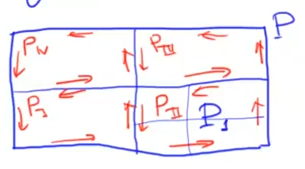
\includegraphics[width=7cm]{assets/04-functions-of-complex-variables/Cauchy-theorem-rectangle-partition.png}
            \end{center}

            
            Режем прямоугольник на 4 части, индексируем как $P^{1}, P^{2}, P^{3}, P^{4}$, строим обходы каждого (против часовой стрелки). Тогда $\alpha(P) = \alpha(P^{1}) + \alpha(P^{2}) + \alpha(P^{3}) + \alpha(P^{4})$, $|\alpha(P)| \leq |\alpha(P^{1})| + |\alpha(P^{2})| + |\alpha(P^{3})| + \alpha(P^{4})$.

            Хотя бы одно из слагаемых $\geq \frac{1}{4} |\alpha(P)|$, назовем такое $P_1$ (индекс уже снизу!). Разрежем его на 4 равные части. Пусть $P_2$ такой, что $|\alpha(P_2)| \geq \frac{1}{4} |\alpha (P_1)|$ и т.д.

            $|\alpha(P_n)| \geq \frac{1}{4^n} |\alpha (P)|$.

            % todo: picture
            \begin{center}
                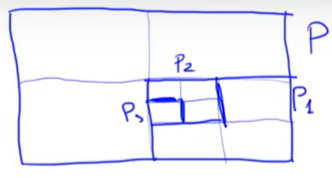
\includegraphics[width=7cm]{assets/04-functions-of-complex-variables/Cauchy-theorem-rectangle-partition-2.png}
            \end{center}

            Берем $a$ из $P_n$:

            $f(z) = f(a) + f'(a) (z - a) + o(z - a)$

            $\alpha (P_n) = \int_{P_n} { f(z) dz } = \underbrace{\int_{P_n} { f(a) dz }}_{= 0 \text{, по 1-ому док-ву}} + \underbrace{\int_{P_n} { f'(a) (z - a) dz }}_{= 0 \text{, по 1-ому док-ву}} + \int_{P_n} { o(z - a) dz }$


            \begin{center}
                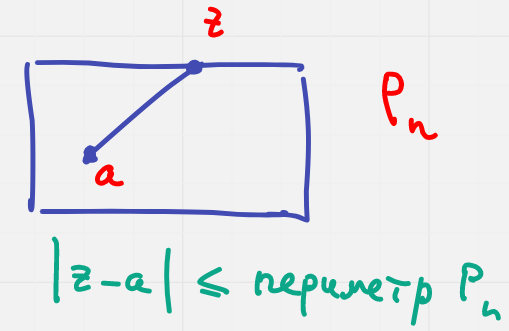
\includegraphics[width=7cm]{assets/04-functions-of-complex-variables/Cauchy-theorem-rectangle-partition-3.png}
            \end{center} 


            $o(z - a) = (z - a) \cdot \beta (z - a)$, где $\beta(z - a) \underbrace{\rightarrow}_{z \rightarrow a} 0$

            $\left| \int_{P_n} {(z - a) \beta (z - a) dz} \right| \leq max_{z \in P_n} { |z - a| \cdot |\beta (z - a)| } \cdot \underbrace{l(P_n)}_{\text{периметр}} \leq max_{z \in P_n} { |\beta (z - a)| } \cdot \frac{l(P)}{2^n} \cdot \frac{l(P)}{2^n} \implies$

            $\implies \frac{|\alpha (P)|}{4^n} \leq |\alpha(P_n)| \leq \frac{l(P) \cdot l(P)}{4^n} \cdot max_{z \in P_n} |\beta (z - a)| \implies max_{z \in P_n} |\beta (z - a)| \geq \frac{|\alpha (P)|}{l(P) \cdot l(P)} > 0$ -- противоречие, т.к. $\beta(z) \rightarrow 0$ при $z \rightarrow a$.
        }
    \end{enumerate}
\end{proof}
\begin{consequence}
    \begin{enumerate}
        \item {
            Если $f \in H(\Omega)$, то у каждой точки $a \in \Omega$ есть окрестность, в которой существует ф-я $F$, т.ч. $F' = f$ в этой окрестности.

            \begin{proof}
                Пусть $F$ первообразная формы $f(z) dz$. Поймем, что $F' = f$.

                $\frac{\partial F}{\partial x} = f(z), \ \frac{\partial F}{\partial y} = i \cdot f(z) \implies \frac{\partial F}{\partial x} + i \frac{\partial F}{\partial y} = 0 \implies \frac{\partial F}{\partial \overline{z}} = 0$
            \end{proof}
        }
        \item {
            $f \in H(\Omega)$, $\gamma$ стягиваемый в $\Omega$ путь $\implies \int_{\gamma} { f(z) dz } = 0$
        }
    \end{enumerate}
\end{consequence}
\begin{theorem}
    $f \in C(\Omega), \ \Delta$ -- прямая параллельная оси координат.

    $f \in H(\Omega \setminus \Delta)$

    Тогда $f(z) dz$ локально точная.
\end{theorem}

\begin{proof}
    Надо проверять, что интеграл по довольно маленькому прямоугольнику (со стороронами паралл. осям) это 0.

    \begin{center}
        \includegraphics*[width=0.3\textwidth]{assets/04-functions-of-complex-variables/interesting-rectangles-locally-exact-form-without-line.png}
    \end{center}

    Очевидно, что если прямоугольник не пересекает $\Delta$, то там все очевидно. Хотим рассматривать только те, что задевают. Те, что пересекают $\Delta$, можно разбить на две части (верхнюю и нижнюю). По каждой из частей будет 0, тогда и в сумме тоже будет 0. То есть нас вообще интересуют только те прямоугольники, у которых $\Delta$ это одна из сторон. Рассмотрим их:
    
    \begin{center}
        \includegraphics*[width=0.5\textwidth]{assets/04-functions-of-complex-variables/smaller-rectangle-locally-exact-form-without-line.png}
    \end{center}

    $\int_{P_{\epsilon}} { f(z) d z } = 0 \rightarrow_{\epsilon \rightarrow 0} \int_{P} { f(z) dz }$

    $\left|\int_{P} {f(z) dz} - \int_{P_{\epsilon}} { f(z) dz } \right| \leq |\int_{1} + \int_{3}| + |\int_{2}| + |\int_{4}|$

    $\left| \int_{2} {f(z) dz} \right| \leq M \cdot (\text{длина } 2) = M \epsilon$

    $\left| \int_{1} + \int_{3} \right| = \left| \int_{a}^{b} { \left(f (x + i y_0) - f(x + i(y_0 + \epsilon)) \right) dx } \right| \leq \int_{a}^{b} { |\dots| dx } = (*)$

    $f$ непрер. на компакте $\implies$ равномерно непрер.

    $\forall \gamma > 0: \ \exists \epsilon > 0$ если $\rho (\text{аргумент}) < \epsilon \implies |f(\dots) - f(\dots)| < \gamma$, тогда 

    $(*) \leq (b - a) \cdot \gamma$
\end{proof}

\begin{consequence}
    $f: \Omega \rightarrow \mathbb{C}$

    $f \in C(\Omega)$ и $f$ голоморфна в $\Omega$ за исключением мн-ва изолированных точек, тогда форма $f(z) dz$ все равно лок. точная.
\end{consequence}
\begin{proof}
    Рассмотрим окр-ть, в которой ровно одна плохая точка.

    % todo: picture
    Давайте проведем прямую через это точку, тогда работает теорема.
\end{proof}

\begin{definition}
    Индекс кривой отн-но точки $Ind(\gamma, z_0)$.

    $\gamma$ -- замкнутая кривая, не проходящая через точку $z_0$.

    $Ind(\gamma, 0) = \frac{\phi(b) - \phi(a)}{2\pi} \in \mathbb{Z}$ -- кол-во оборотов $\gamma$ вокруг 0.

    $\gamma: [a, b] \rightarrow \mathbb{C}$

    $\gamma(t) = r(t) e^{i \phi(t)}$, $\phi$ -- непрерывна (полярная замена).
\end{definition}

\begin{theorem}
    Пусть $\gamma$ -- замкнутая кривая, не проходящая через 0. Тогда
    
    $\int_{\gamma} { \frac{d z}{z} } = 2\pi i Ind(\gamma, 0)$.
\end{theorem}
\begin{proof}
    Берем параметризацию $r, \phi: [a, b] \rightarrow \mathbb{R}$

    $z(t) = r(t) e^{i \phi(t)}, \ dz = \left( r' e^{i\phi} + ri \phi' e^{i\phi} \right) dt$

    $\frac{dz}{z} = \frac{r'}{r} + i \phi'$

    $\int_{\gamma} { \frac{dz}{z} } = \int_{a}^{b} { \left( \frac{r'(t)}{r(t)} + i \phi'(t) \right) dt } = \left( ln (r(t)) + i \phi(t) \right)|_{t = a}^{t = b} = i (\phi(b) - \phi(a)) = 2 \pi i Ind(\gamma, 0)$
\end{proof}

\begin{consequence}
    Пусть $\gamma$ -- замкнутая кривая, не проходящая через точку $a$. Тогда

    $\int_{\gamma} { \frac{dz}{z - a} = 2 \pi i Ind (\gamma, a) }$.
\end{consequence}

\begin{theorem}
    (интегральная формула Коши).

    $f \in H(\Omega)$

    $\gamma$ -- стягиваемая в $\Omega$ кривая, не проходящая через $a \in \Omega$.

    Тогда $\int_{\gamma} { \frac{f(z) dz}{z - a} } = 2 \pi i f(a) Ind(\gamma, a)$
\end{theorem}
\begin{proof}
    $g(z) = \begin{cases}
        \frac{f(z) - f(a)}{z - a}, \ \text{при } z \not = a, \\
        f'(a), \ \text{иначе}
    \end{cases}$

    $g \in C(\Omega)$

    $g \in H(\Omega \setminus \{ a \})$

    $\implies g(z) dz$ -- локально точкая форма $\implies \int_{\gamma} {g(z) dz} = 0$, так как $\gamma$ -- стягиваемая

    $\implies 0 = \int_{\gamma} { \frac{f(z) dz}{z - a} } - \int_{\gamma} { \frac{f(a) dz}{z - a} } \implies \int_{\gamma} { \frac{f(z) dz}{z - a} } = f(a) \cdot \int_{\gamma} { \frac{dz}{z - a} } = f(a) \cdot 2 \pi i \cdot Ind(\gamma, a)$
\end{proof}
\begin{example}
    % todo: picture !!!
    Берем круг. $f$ -- голоморфна в окр-ти этого круга.

    $\int_{\text{окр.}} { \frac{f(z)}{z - a} dz } = \begin{cases}
        0, \ \text{ если $a$ вне круга} \\
        f(a) \cdot 2 \pi i, \ \text{ если $a$ внутри круга }
    \end{cases}$
\end{example}

\begin{remark}
    Обозначение.

    $\mathbb{D} = \{ |z| \leq 1 \}$ -- единичный круг.

    $\mathbb{T} = \{ |z| = 1 \}$ -- единичная окружность, обход против часовой стрелки.

    $r\mathbb{T} + a = \{ |z - a| = r \}$
\end{remark}

\begin{theorem}
    $f \in H(r \mathbb{D}) \implies f$ аналитична ($=$ функция раскладывается в ряд) в этом круге.
\end{theorem}

\begin{proof}
    % todo: picture
    В нашем круге радиуса $r$ берем еще два круга с тем же центром, но меньшими радиусами ($r > r_1 > r_2 > 0$). Берем $z: \ |z| < r_2$ -- точка внутри наименьшего круга. Хотим интегрировать по средней окружности.

    $f(z) = \frac{1}{2 \pi i} \int_{r_1 \mathbb{T}} { \frac{f(\zeta) d \zeta }{\zeta - z} }$

    $\frac{1}{\zeta - z} = \frac{1}{1 - \frac{z}{\zeta}} \cdot \frac{1}{\zeta} = \sum_{n=0}^{\infty} \frac{z^n}{\zeta^{n+1}} = (*)$ равномерно сх-ся, так как $\left| \frac{z}{\zeta} \right| \leq \frac{r_2}{r_1} < 1$

    $(*) = \frac{1}{2\pi i} \int_{r_1 \mathbb{T}} { \sum_{n=0}^{\infty} \frac{f(\zeta)}{\zeta^{n+1}} z^n d\zeta } = \frac{1}{2\pi i} \sum_{n=0}^{\infty} z^n \underbrace{\int_{r_1 \mathbb{T}} {\frac{f(\zeta)}{\zeta^{n+1}} d\zeta}}_{=: a_n \cdot 2\pi i} = \sum_{n=0}^{\infty} {a_n z^n}$
\end{proof}



\begin{consequence}
    \begin{enumerate}
        \item {
            Если $f \in H(r \mathbb{D})$ и $0 < r_1 < r$, то
    
            $\frac{n!}{2 \pi i} \cdot \int_{r_1 \mathbb{T}} { \frac{f(z)}{z^{n+1}} dz } = f^{(n)} (0)$
        }
        \item {
            $f \in H(r \mathbb{D} + a), \ 0 < r_1 < r \implies \frac{n!}{2 \pi i} \int_{r_1 \mathbb{T} + a} { \frac{f(z)}{(z - a)^{n + 1}} dz } = f^{(n)} (a)$

            $z = w + a$

            $g(w) = f(w + a)$

            $g^{(n)} (0) = \frac{n!}{2 \pi i} \cdot \int_{r_1 \mathbb{T}} { \frac{g(w)}{w^{n + 1}} dw }$
        }
        \item {
            $f: \Omega \rightarrow \mathbb{C}$

            Тогда $f$ -- голоморфна в $\Omega \Leftrightarrow f$ -- аналитична в $\Omega$.

            % todo: picture
        }
        \item {
            $f \in H(\Omega) \implies f$ -- бесконечно диффиренцируема.
        }
        \item {
            $f \in H(\Omega) \implies f' \in H(\Omega)$
        }
        \item {
            \begin{definition}
                $g: \mathbb{R}^n \rightarrow \mathbb{R}$ -- гармоническая, если $\frac{\partial^2 g}{\partial x_1^2} + \frac{\partial^2 g}{\partial x_2^2} + \dots + \frac{\partial g}{\partial x_n^2} = 0$.
            \end{definition}
            
            Продолжаем свойство:

            $f \in H(\Omega) \implies Re (f)$ и $Im(f)$ -- гармонические функции.
            
            \begin{proof}
                $\frac{\partial^2 Re(f)}{\partial x^2} = \frac{\partial}{\partial x} \left( \frac{\partial Re (f)}{\partial x} \right) = \frac{\partial}{\partial x} \left( \frac{\partial Im(f)}{\partial y} \right) = \frac{\partial}{\partial y} \left( \frac{\partial Im(f)}{\partial x} \right) = \frac{\partial}{\partial y} \left( - \frac{\partial Re(f)}{\partial y} \right) = - \frac{\partial^2 Re(f)}{\partial y^2}$

                про $Im(f)$ аналогично доказывается.
            \end{proof}
        }
    \end{enumerate}
\end{consequence}

\begin{remark}
    Если $g: \Omega \rightarrow \mathbb{R}$ гармоническая ф-я, то существует единств. (с точностью до прибавления $const \in \mathbb{R}$) гармоническая ф-я $h: \Omega \rightarrow \mathbb{R}$, т.ч. $g + i h \in H(\Omega)$
\end{remark}

\begin{theorem}
    \textbf{Мореры}.

    $f \in C(\Omega)$. Если $f(z) dz$ локально точная, то $f \in H(\Omega)$.
\end{theorem}
\begin{proof}
    Возьмем $a \in \Omega$. Существует окр-ть $a$, что для $f$ в ней есть первообразная $F$ (т.е. $F' = f$ в $U$). 
    
    Тогда $F \in H(U) \implies F' = f \in H(U)$ -- это локальное свойство, поэтому на всей $\Omega$ тоже будет гомоморфность.
\end{proof}

\begin{consequence}
    $f \in C(\Omega), \ \Delta$ -- прямая, параллельная оси координат.

    $f \in H(\Omega \setminus \Delta)$. Тогда $f \in H(\Omega)$.
\end{consequence}
\begin{proof}
    $f \in C(\Omega)$ и $f \in H(\Omega \setminus \Delta) \implies f(z) dz$ локально точная в $\Omega \underbrace{\implies}_{\text{т. Мореры}} f \in H(\Omega)$.
\end{proof}

\begin{theorem}
    (интегральная формула Коши).

    $f \in H(\Omega)$

    $K \subset \Omega$ -- компакт, граница которого -- конечное число кусочно-гладких замкнутых кривых. Тогда 

    \begin{enumerate}
        \item {
            $\int_{\partial K} { f(z) dz } = 0$
        }
        \item {
            Если $a \in Int (K)$, то $\int_{\partial K} { \frac{f(z)}{z - a} dz } = 2 \pi i f(a)$.
        }
    \end{enumerate}
\end{theorem}
\begin{proof}
    \begin{enumerate}
        \item {
            Пишем \textbf{формулу Грина}.

            $\int_{\partial K} { f(z) dz } = \int_{\partial K} { f(z) dx + i \cdot f(z) dy } \underbrace{=}_{\text{Грин}} \int_{K} { \left( i \cdot \frac{\partial f}{\partial x}  - \frac{\partial f}{\partial y} \right) dx dy } = $
            
            $ = i \cdot \int_{K} {\left( \frac{\partial f}{\partial x} + i \frac{\partial f}{\partial y} \right) dx dy} = 2 i \int_{K} { \frac{\partial f}{\partial \overline{z}} d \lambda_2 } = 0$.
        }
        \item {
            % todo: picture !!!
            Берем круг, содержащий $a$, не вылезающий за границу формы $B_r(a)$.
            
            $\tilde{K} = K \setminus B_r(a)$ -- компакт.

            $\frac{f(z)}{z - a} \in H(\Omega \setminus \{ a \}), \ \tilde{K} \subset \Omega \setminus \{ a \}$.

            $0 = \int_{\partial \tilde{K}} { \frac{f(z)}{z - a} dz } = \int_{\partial K} { \frac{f(z)}{z - a} dz } - \underbrace{\int_{r \mathbb{T} + a} { \frac{f(z)}{z - a} dz }}_{= 2\pi i f(a)}$.
        }
    \end{enumerate}
\end{proof}
\begin{exerc}
    $f \in H(r \mathbb{D})$ и $f \in C(Cl (r \mathbb{D}))$

    $a \in \mathbb{D}$.
    
    Доказать, что $\int_{r \mathbb{T}} { \frac{f(z)}{z - a} dz } = 2 \pi i f(a)$
\end{exerc}

\begin{theorem}
    $f \in C(\Omega)$. Следующие условия равносильны (равносильность всех утверждений, так или иначе, уже доказывалась ранее):

    \begin{enumerate}
        \item {
            $f \in H(\Omega)$
        }
        \item {
            $f(z) dz$ -- локально точная в $\Omega$
        }
        \item {
            В окр-ти каждой точки у $f$ есть первообразная
        }
        \item {
            $f$ аналитична в $\Omega$
        }
        \item {
            $\int{f(z) dz} = 0$ по любому достаточно малому прямоугольнику со сторонами параллельными осям
        }
        \item {
            $f(z) dz$ -- замкнутая и частн. производные по $x$ и $y$ непрерывны.
        }
    \end{enumerate}
\end{theorem}

\begin{theorem}
    \textbf{Неравенство Коши}.

    $f \in H(R \mathbb{D}), \ 0 < r < R$.

    $f(z) = \sum_{n=0}^{\infty} {a_n z^n}$. Тогда $|a_n| \leq \frac{M(r)}{r^n}$, где $M(r) := \max_{|z| = r} |f(z)|$.
\end{theorem}
\begin{theorem}
    $a_n = \frac{1}{2 \pi i} \int_{|z| = r} { \frac{f(z)}{z^{n + 1}} dz }$

    $|a_n| = \frac{1}{2 \pi} \left| \int_{|z| = r} { \frac{f(z)}{z^{n+1}} dz } \right| \leq \frac{1}{2 \pi} \cdot \max_{|t| = r} \left|\frac{f(z)}{z^{n+1}}\right| \cdot 2 \pi r = \frac{M(r)}{r^{n + 1}} \cdot r = \frac{M(r)}{r^n}$
\end{theorem}

\begin{theorem}
    \textbf{Луивилля}.

    Если $f \in H(\mathbb{C})$ и $f$ -- ограничена, то $f = const$.
\end{theorem}
\begin{proof}
    $f$ -- ограничена $\implies |f| \leq M$.
    
    $f \in H(\mathbb{C}) \implies f(z) = \sum_{n=0}^{\infty} { a_n z^{n} }$ и ряд сходится $\forall z \in \mathbb{C} \underbrace{\implies}_{\text{нер-во Коши}} |a_n| \leq \frac{M_r}{r^n} \leq \frac{M}{r^n} \underbrace{\rightarrow}_{r \rightarrow +\infty} 0 \implies a_n = 0: \ \forall n \geq 1$
\end{proof}

\begin{remark}
    $\sin$ и $\cos$ неограничены в $\mathbb{C}$.
\end{remark}

\begin{definition}
    Целая функция -- функция, голоморфная в $\mathbb{C}$.
\end{definition}

\begin{theorem}
    \textbf{Основная теорема алгебры}.

    $P$ -- многочлен степени $\geq 1$. Тогда у $P$ есть хотя бы один корень.
\end{theorem}
\begin{consequence}
    Если $deg P = n$, то $P(z) = c(z - z_1)(z - z_2) \dots (z - z_n)$ для некоторых $z_1, z_2, \dots z_n \in \mathbb{C}$.
\end{consequence}
\begin{proof}
    Если $z_1$ -- корень $P$, то $P(z) = (z - z_1) \cdot Q(z)$, где $deg Q = n - 1$.
\end{proof}
\begin{proof}
    Основной теоремы алгебры.

    От противного:

    пусть $P(z) \not = 0 \ \forall z \in \mathbb{C}$. Тогда $f(z) = \frac{1}{P(z)} \in H(\mathbb{C})$.

    Докажем, что $f$ -- ограниченная функция.

    $P(z) = z^n + a_{n-1} z^{n-1} + \dots + a_1 z + a_0$

    $R := 1 + |a_{n-1}| + |a_{n-2}| + \dots + |a_1| + |a_0|$. Пусть $|z| \geq R, \ |P(z)| \geq |z|^n - |a_{n-1}| |z|^{n-1} - \dots - |a_1| |z| - |a_0| \geq |z|^n - |z|^{n-1} (|a_{n-1}| + |a_{n-2}| + \dots + |a_0|) = \underbrace{|z|^{n-1}}_{\geq 1} \underbrace{(|z| - |a_0| - |a_1| - \dots - |a_{n-1}|)}_{\geq 1} \implies |P(z)| \geq 1$ при $|z| \geq R \implies |f(z)| \leq 1$ при $|z| \geq R$.

    Докажем, что при $|z| \leq R, \ |f(z)|$ -- ограничена.

    $f \in H(\mathbb{C}) \implies f$ непрер. в $\mathbb{C} \implies f$ непрер. в $\{ |z| \leq R \}$ -- компакт $\implies |f|$ огр. в $\{ |z| \leq R \}$.

    Тогда по т. Луивиля $f(z) = const \implies P(z) = \frac{1}{const}$, что противоречит условию, что $P(z)$ -- многочлен степени $\geq 1$.
\end{proof}


\Subsection{Теоремы единственности}
\begin{theorem}
    $f \in H(\Omega)$, $\Omega$ -- область, $z_0 \in \Omega$. След. условия равносильны:

    \begin{enumerate}
        \item {
            $f^{(n)} (z_0) = 0 \ \forall n = 0, 1, 2, \dots$
        }
        \item {
            $f = 0$ в некоторой окр-ти точки $z_0$.
        }
        \item {
            $f \equiv 0$ в $\Omega$
        }
    \end{enumerate}
\end{theorem}


\begin{lemma}
    $\Omega$ -- область в метрическом пространстве, $E \subset \Omega$, т.ч. $E \not = \emptyset, \ E$ -- открыто в $\Omega$, $E$ -- замкнуто в $\Omega$. Тогда $E = \Omega$.
\end{lemma}
\begin{proof} Леммы.

    Пусть $\Omega \setminus E \not = \emptyset$, берем $a \in E$ и $b \in \Omega \setminus E$. Возьмем путь $\gamma$, соединяющий эти точки.

    $\gamma: [\alpha, \beta] \rightarrow \Omega$, т.ч. $\gamma(\alpha) = a, \ \gamma(\beta) = b$. $\gamma$ -- непрер. $\implies \gamma^{-1} (E)$ -- открыто, $\gamma^{-1}(\Omega \setminus E)$ -- открыто $\implies \gamma^{-1}(E)$ -- открыт. и замкнут. подмн-во $[\alpha, \beta], \ \alpha \in \gamma^{-1}(E), \ \beta \not \in \gamma^{-1}(E)$.

    $s := \sup{\gamma^{-1} (E)}$ из замкн. $s \in \gamma^{-1} (E) \implies s < \beta$.

    % todo: picture

    Возьмем окр-ть $s$, т.ч. $(s - \delta, s + \delta) \subset \gamma^{-1}(E) \cap (\alpha, \beta) \implies $ в $\gamma^{-1}(E)$ есть точки $> s \implies s $ не $\sup$. Противоречие. 
\end{proof}

\begin{proof}
    Теоремы.

    $(3) \implies (2) \implies (1)$ -- очевидно.

    $(1) \implies (2)$ -- почти очевидно:

    % todo: picture
    Берем $z_0 \in \Omega$ и $B_r(z_0) \subset \Omega$, тогда в круге $|z - z_0| < r: $ $f$ раскл. в свой ряд Тейлора $\implies$ в нем $f \equiv 0$.

    $(2) \implies (3)$:

    $E := \{ z \in \Omega: \ \text{в некоторой окр-ти точки } z, \ f = 0 \}$

    $z_0 \in E$ по условию $\implies E \not = \emptyset$.

    $E$ -- открыто. Если $w \in E$, то в круге $|z - w| < r, \ f = 0$.
    % todo: picture

    $\forall z$ из этого круга есть круг меньшего радиуса, содерж. $\{ |z - w| < r \}$, в нем $f = 0$.

    $E$ -- замкнуто. Пусть $z_*$ -- предельная точка $E$, то есть $z_n \in E$ и $\lim{z_n} = z_*$. $f^{(m)} (z_n) = 0 \ \forall m, \ \forall n$ (так как есть $(2) \implies (1)$). По непрерывности $f^{(m)} \ f^{(m)} (z_*) = \lim{f^{(m)} (z_n)} = 0 \underbrace{\implies}_{(1) \implies (2)} z_* \in E$.

    Тогда по лемме $E = \Omega$.
\end{proof}


\begin{consequence}
    $f, g \in H(\mathbb{C})$, т.ч. $f(z) = g(z)$ в окр-ти точки $z_0 \in \Omega \implies f \equiv g$.
\end{consequence}



\begin{theorem}
    \textbf{О среднем}.

    $f \in H(\Omega)$ и $a \in \Omega$, причем $\{ |z - a| \leq r \} \subset \Omega$, тогда $f(a) = \frac{1}{2\pi} \cdot \int_{0}^{2\pi} { f(a + r e^{i \phi}) d \phi }$ (т.е. среднее значение на окружности радиуса $r$ с центром в $a$ равно $f(a)$).
\end{theorem}
\begin{proof}
    $f(a) = \frac{1}{2 \pi i}\int_{|z - a| = r}{ \frac{f(z)}{z - a} dz } = \frac{1}{2 \pi i} \int_{0}^{2\pi} { \frac{f(a + r e^{i \phi})}{r e^{i \phi}} r e^{i \phi} i d \phi }$, где $z = a+re^{i\phi}, \ dz = r e^{i \phi} i d \phi$.
\end{proof}

\begin{consequence}
    $f \in H(\Omega), \ a \in \Omega, \ \{ |z - a| \leq r \} \subset \Omega$. Тогда $f(a) = \frac{1}{\pi r^2} \int_{|z-a|\leq r} { f(z) d \lambda_2 }$.
\end{consequence}
\begin{proof}
    $\int_{|z-a| \leq r} { f(z) d \lambda_2 } = \int_{0}^{r} { \int_{0}^{2\pi} {f(a + \rho e^{i\phi}) \rho d \phi } d \rho } = \int_{0}^{r} { 2 \pi f(a) \rho \ d \rho } =$
    
    $= 2 \pi f(a) \frac{r^2}{2} = \pi r^2 f(a)$.
\end{proof}

\begin{theorem}
    \textbf{Принцип максимума}.

    $f \in H(\mathbb{C}), \ a \in \Omega$. Если $|f(a)| \geq |f(z)| \ \forall z$ из окр-ти точки $a$, то $f \equiv const$.
\end{theorem}
\begin{proof}
    Пусть $|f(a)| =: M$. Домножим $f$ на $e^{i \alpha}$ так, что $f(a) = M > 0$.

    $|f(a)| = M = \frac{1}{2\pi} \left|\int_{0}^{2\pi} { f(a + r e^{i \phi}) d \phi }\right| \leq \frac{1}{2 \pi} \int_{0}^{2\pi} { |f(a + r e^{i \phi})| d \phi} \leq \frac{1}{2\pi} \int_{0}^{2\pi} { M \ d \phi } = M$.

    Все нер-ва обращаются в равенства $\implies |f(a + r e^{i \phi})| = M \ \forall \phi \ \forall$ маленьких $r$.

    $Re (f(a)) = M = \frac{1}{2\pi} \int_{0}^{2\pi} { Re(f(a + r e^{i \phi})) d \phi } \leq \frac{1}{2 \pi} \int_{0}^{2\pi} { |f(a + r e^{i \phi})| d \phi } \leq M$. Это все равенства $\implies Re (f(a + r e^{i \phi})) = |f(a + r e^{i \phi})| = M \implies f(z) = M$ в окр-ти точки $a \underbrace{\implies}_{\text{т. о единственности}} f(z) \equiv const$.
\end{proof}


\begin{consequence}
    $f \in H(\Omega), \ \Omega$ -- огранич. область, $f \in C(Cl (\Omega))$. Тогда $|f|$ достигает своего $\max$ на границе $\Omega$.
\end{consequence}

\begin{proof}
    $Cl (\Omega)$ -- компакт, $|f|$ непрер. на компакте $\implies$ в какой-то точке $a \in Cl (\Omega)$ достигает $\max$.

    Если $a \in \Omega$, то по принципу максимума $f \equiv const$, значит на границе то же самое значение.

    Если $a \not \in \Omega$, то это точка на границе.
\end{proof}



\begin{definition}
    $f \in H(\Omega), \ a \in \Omega, \ a$ -- ноль функции $f$, если $f(a) = 0$.
\end{definition}

\begin{theorem}
    $f \not \equiv 0, \ f \in H(\Omega), \ a \in \Omega, \ f(a) = 0$. Тогда существует $m \in \mathbb{N}$ и $g \in H(\Omega)$, т.ч. $g(a) \not = 0$ и $f(z) = (z - a)^{m} \cdot g(z)$.
\end{theorem}
\begin{proof}
    Разложим $f$ в ряд Тейлора в окр-ти точки $a$.

    $f(z) = \sum_{n=0}^{\infty} { \frac{f^{(n)} (a)}{n!} \cdot (z - a)^{n} }$, $m := \min \{ n : \ f^{(n)} (a) \not = 0 \}$.

    $g(z) = \begin{cases}
        \frac{f(z)}{(z - a)^{m}}, \ z \not = a \\
        \frac{f^{(m)} (a)}{m!}, \ z = a
    \end{cases}$

    $g \in H(\Omega \setminus \{a\})$, $g$ -- непрерывная в точке $a$,  $\implies g \in H(\Omega)$.

    $g(z) = \sum_{n=m}^{\infty} { \frac{f^{(n)} (a)}{n!} (z - a)^{n - m} } \underbrace{\rightarrow}_{z \rightarrow a} \frac{f^{(m)} (a)}{m!}$
\end{proof}


\begin{consequence}
    \begin{enumerate}
        \item {
            Если $f \in H(\Omega)$ и $a \in \Omega$ -- ноль функции $f$, то $\exists U_a$ -- кор-ть точки $a$, т.ч. $f(z) \not = 0 \ \forall z \in U^{\circ}_a$ (проколотая окр-ть).

            \begin{proof}
                $f(z) = (z - a)^m g(z), \ g(a) \not = 0$ из теоремы.

                $g$ -- непрер. в точке $a \implies g(z) \not = 0$ в окр-ти точки $a \implies f(z) = (z - a)^m g(z) \not = 0$ в прокол. окр-ти точки $a$.
            \end{proof}
        }
        \item {
            Если $f, g \in H(\Omega)$ и $f g \equiv 0$, то либо $f \equiv 0$, либо $g \equiv 0$.

            \begin{proof}
                Пусть $f \not \equiv 0$. Если $f(z) \not = 0 \ \forall z$, то $g \equiv 0$. Иначе найдется $a \in \Omega$, т.ч. $f(a) = 0 \implies f(z) \not = 0, \ \forall z \in U^{\circ}_a \implies g(z) = 0 \ \forall z \in U^{\circ}_a \implies g \equiv 0$.
            \end{proof}
        }
    \end{enumerate}
\end{consequence}


\begin{theorem}
    \textbf{Единственности}.

    $f, g \in H(\Omega)$ и $z_n \in \Omega$, $z_n$ -- различные, т.ч. $f(z_n) = g(z_n)$. Если $\lim {z_n} \in \Omega$, то $f \equiv g$.
\end{theorem}

\begin{consequence}
    $f, g \in H(\Omega), \ A := \{ z \in \Omega: \ f(z) = g(z) \}$. Если какая-то предельная точка мн-ва $A$ лежит в $\Omega$, то $f \equiv g$.
\end{consequence}

\begin{proof}
    Теоремы.

    $h(z) = f(z) - g(z)$. По условию $h \in H(\Omega)$ и $h(z_n) = 0$. $a := \lim{z_n}$, по непрерывности $h(a) = 0 \underbrace{\implies}_{\text{по следствию 1}} \exists U_a$, т.ч. $h(z) \not = 0 \ \forall z \in U^{\circ}_a$, но $z_n$ начиная с некоторого места лежат в $U_a$. 
\end{proof}



\begin{consequence}
    $\sin^2{z} + \cos^2{z} = 1, \ \forall z \in \mathbb{C}$.
\end{consequence}



\Subsection{Аналитическое продолжение}

\begin{definition}
    % todo: picture

    $f_1 \in H(\Omega_1), \ f_2 \in H(\Omega_2)$.

    $\Delta$ -- компонента связности $\Omega_1 \cap \Omega_2 \not = \emptyset$.

    \begin{center}
        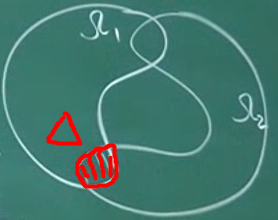
\includegraphics[width=5cm]{assets/04-functions-of-complex-variables/analitical-extension-difinition.png}
    \end{center}

    $f_2$ непосредственное аналитическое продолжение $f_1$ через $\Delta$, если $f_1(z) = f_2(z) \ \forall z \in \Delta$.
\end{definition}
\begin{remark}
    \begin{enumerate}
        \item {
            При фиксации $\Omega_1, \ \Omega_2, \Delta, f_1$, функция $f_2$ определена однозначно.

            \begin{proof}
                $g$ -- непоср. аналитическое продолжение $f_1$:
            
                $g(z) = f_1(z) = f_2(z) \ \forall z \in \Delta$
            
                $g, f_2 \in H(\Omega_2) \underbrace{\implies}_{\text{по т. единственности}} f_2 \equiv g$.
            \end{proof}            
        }
        \item {
            Для другой компоненты продолжение может быть другим (тут понятнее на картинке, добавьте, плиз).
        }
    \end{enumerate}
\end{remark}

\begin{definition}
    $f \in H(\Omega), \ \tilde{f} \in H(\tilde{\Omega})$.

    $\tilde{f}$ -- аналитическое продолжение $f$ на цепочке областей, если $\exists \Omega_1, \dots \Omega_n$ и $f_1 \in H(\Omega_1), \dots , f_n \in H(\Omega_n)$, т.ч. $f_1$ -- непосредственное аналитическое продолжение $f$, $f_2$ -- непосредственное аналитическое продолжение $f_1, \dots, \tilde{f}$ -- непосредственное аналитическое продолжение $f_n$.
    % todo: picture

    \begin{center}
        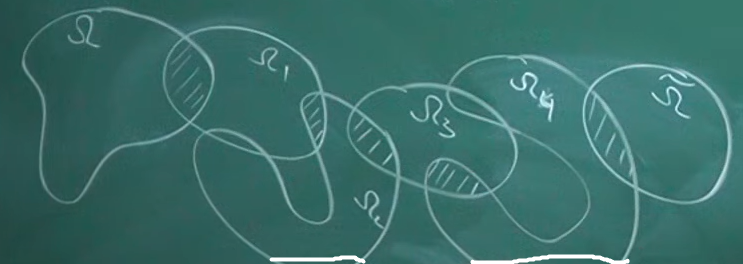
\includegraphics[width=11cm]{assets/04-functions-of-complex-variables/analitical-multiple-extension.png}
    \end{center}
\end{definition}



\begin{remark}
    Рассмотрим всевозможные пары $(f, \Omega)$, т.ч. $f \in H(\Omega)$, тогда существование аналитического продолжения по цепочке областей -- отношение эквивалентности на мн-ве таких пар. 
\end{remark}


\begin{definition}
    Полная аналитическая функция -- класс эквивалентности. 

    $F$ -- полная аналитическая ф-я. $M := \bigcup_{(f, \Omega) \in F} {\Omega}$ -- область определения (существования) $F$.
\end{definition}

\begin{statement}
    $M$ -- область.
\end{statement}
\begin{proof}
    \textbf{Открытость}: объединения открытых -- открытое.

    \textbf{Линейная связность}: $a, b \in M \implies a \in \Omega, b \in \tilde{\Omega}$. $(f, \Omega), \ (\tilde{f}, \tilde{\Omega})$ связана аналитическим продолжением по цепочке, будем переходить по соотвествующим областям и дойдем из $a$ в $b$.
\end{proof}


\begin{definition}
    $F$ -- полная аналитическая функция, $M$ -- область определения $F$, $z \in M$.

    $F(z) := \{ f(z): \ (f, \Omega) \in F \ \land \ z \in \Omega \}$.
\end{definition}

\begin{theorem}
    \textbf{Пуанкаре-Вольтерры}.

    $F(z)$ -- не более чем счетное мн-во.
\end{theorem}

\begin{example}
    $\underbrace{f(z)}_{\frac{1}{1-z}} = \sum_{n=0}^{\infty} {z^n}$ -- ряд сх-ся при $|z| < 1$

    % todo: picture.

    $\frac{1}{1 - z} = \frac{1}{(1-a) - (z - a)} = \frac{1}{1-a} \cdot \frac{1}{1 - \frac{z-a}{1-a}} = \frac{1}{1-a} \cdot \sum_{n=0}^{\infty} { \frac{(z-a)^n}{(1-a)^n} } = \sum_{n=0}^{\infty} { \frac{(z-a)^n}{(1-a)^{n+1}} }$

    $\left| \frac{z-a}{1-a} \right| < 1$ -- круг сходимости ряда.

    $|z-a| < |1-a|$

    % todo: picture
\end{example}


\begin{definition}
    $\sum_{n=0}^{\infty} { c_n \cdot (z - z_0)^n }$, $R$ -- радиус сх-ти ряда.

    % todo: picture

    Берем точку $w$ на границе круга ($|w - z_0| = R$). $w$ -- правильная точка, если найдется $U_w$ -- окр-ть точки $w$ и $g \in H(U_w)$ являющаяся непосредственным продолжением $f$. 
\end{definition}

\begin{definition}
    Особая точка -- точка, не являющаяся правильной. 
\end{definition}

\begin{theorem}
    На границе круга сх-ти лежит хотя бы одна особая точка.
\end{theorem}
\begin{proof}
    От противного. 

    Пусть все точки правильные $|z| = R$ -- правильные.

    $f(z) = \sum_{n=0}^{\infty} { c_n z^n }, \ R$ -- радиус сх-ти.

    $\forall w: \ |w| = R$ -- правильная, тогда найдется $B_{r_w} (w)$ и $g \in H(B_{r_w} (w))$, т.ч. $f = g$ на пересечении $\{ |z| < R \} \cap \{ |z - w| < r_w \}$.

    То есть круги $B_{r_w}(w)$ покрывают окр-ть $|w| = R$. Это компакт, выберем конечное подпокрытие. 

    % todo: picture

    По лемме Лебега $\exists \epsilon > 0: \ B_{\epsilon} (w)$ целиком содержится в элементе подпокрытия.

    $\{ |z| < R + \epsilon \} \subset \{ |z| < R \} \cup$ конечное подпокрытие. 

    $h(z) := \begin{cases}
        f(z), \ |z| < R \\ 
        g_{w_j} (z), \ |z - w_j| < r_{w_j}
    \end{cases} \in H(\{ |z| < R + \epsilon \})$.

    % todo: picture
    $g(z) = \sum_{n=0}^{\infty} { c_n z^n }$ -- ряд Тейлора для $g$, он сх-ся в круге $|z| < R + \epsilon$.

    Противоречие тому, что радиус сходимости был $R$.
\end{proof}

\begin{example}
    \begin{enumerate}
        \item {
            $f(z) = \sum_{n=1}^{\infty} { \frac{z^n}{n^2} }$ сх-ся при $|z| \leq 1$.

            $f'(z) = \sum_{n=1}^{\infty} { \frac{z^{n-1}}{n} }$

            $(zf'(z))' = \sum_{n=0}^{\infty} { z^{n-1} } = \frac{1}{1-z}$
        }
        \item {
            $\sum_{n=0}^{\infty} { z^{2^n} }$ -- сх-ся при $|z| < 1$, все точки $|z| = 1$ -- особые. 
            % todo: picture
        }
    \end{enumerate}
\end{example}


Начало 4-ого семестра.

% Начало 4 семестра
\begin{theorem}
    $f \in H(\Omega)$, \ $\Omega$ -- односвязная, $f \not = 0$ в $\Omega$.

    Тогда существует $g \in H(\Omega)$, т.ч. $e^{g(z)} = f(z)$ и $g$ -- единственна с точностью до аддит. константы $2 \pi i k, \ k \in \mathbb{Z}$.
\end{theorem}

\begin{proof}
    \textbf{Существование}:

    $\frac{f'}{f} \in H(\Omega) \implies $ есть первообразная $g \in H(\Omega)$. 
    
    Подберем константу так, что $e^{g(z_0)} =  f(z_0)$ для некоторого $z_0 \in \Omega$. 

    Покажем, что $g$ подходит: $h(z) := e^{-g(z)} \cdot f(z)$.

    Хотим доказать, что $h \equiv 1$. Знаем, что $h(z_0) = 1$ и
    
    $h'(z) = f'(z) e^{-g(z)} + f(z) e^{-g(z)} (-g'(z)) = e^{-g(z)} \left( f'(z) - f(z) \frac{f'(z)}{f(z)} \right) \equiv 0$.

    \textbf{Единственность}:

    Пусть $e^{g(z)} = f(z) = e^{\tilde{g}(z)} \implies e^{g(z) - \tilde{g}(z)} \equiv 1 \implies \underbrace{g(z) - \tilde{g}(z)}_{\in H(\Omega) \subset C(\Omega)} = 2 \pi i k_{z}: \ k_{z} \in \mathbb{Z} \implies g(z) - \tilde{g}(z) = 2 \pi i k$
\end{proof}

\begin{consequence}
    Пусть $0 \not \in \Omega$ -- односвязна, тогда существует единственный с точностью до $+ 2 \pi i k$ функция $g \in H(\Omega)$, т.ч. $e^{g(z)} = z$.
\end{consequence}

\begin{remark}
    $g(z) = \ln{|z|} + i \arg{z}$
\end{remark}

\begin{remark}
    Обозначение:

    $Ln(z) = \ln{|z|} + i Arg(z)$

    % todo: picture

    ветви логарифма
\end{remark}


\begin{properties}
    \begin{enumerate}
        \item $e^{Ln(z)} = z: \ \forall z \not = 0$
        \item $Ln(z w) = Ln(z) + Ln(w)$
        \item $Ln(z) = \ln{|z|} + i Arg(z)$, где $Arg(z) = \{ \arg{z} + 2 \pi i k: \ k \in \mathbb{Z} \}$
    \end{enumerate}
\end{properties}

\begin{remark}
    Св-во 2 для ветви может быть неверно.

    Берем конкретную ветку и точку:
    % todo: picture
    $0 < \arg < 2 \pi$

    $Ln(-i) = \underbrace{\ln{|-i|}}_{=0} + i Arg(-i) = \frac{3\pi i}{2}$

    $Ln((-i)^2) = Ln(-1) = \ln{|-1|} + i Arg(-1) = \pi i$

    Но $\pi i \not = \frac{3 \pi i}{2} + \frac{3 \pi i}{2}$
\end{remark}

\begin{remark}
    $z^p := e^{p Ln(z)}$ -- полная аналит. функция.

    Если $p \in \mathbb{Z}$, то все однозначно, т.к. $e^{p (2 \pi i k)} = 1$.

    Если $p \in \mathbb{Q}, \ p = \underbrace{\frac{m}{n}}_{\text{несократимая}}$, то $e^{\frac{m}{n} (2 \pi i k)}$ -- принимает $n$ значений.

    Если $p \in \mathbb{C} \setminus \mathbb{Q}$, то $e^{p (2 \pi i k)}$ -- принимает счетное кол-во значений.
\end{remark}



\begin{exerc}
    \begin{enumerate}
        \item Найти $i^i$
        \item Д-ть, что $(z^p)' = \frac{p z^p}{z}$ при $z \not = 0$
        \item $(z w)^p = z^p w^p$ как полные аналитичные функции, но это неверно для ветвей.
    \end{enumerate}
\end{exerc}


\Subsection{Ряды Лорана}

\begin{definition}
    $\sum_{n=-\infty}^{+\infty} a_n (z - z_0)^n$ -- ряд Лорана.

    $\sum_{n = 0}^{\infty} a_n (z - z_0)^n$ -- правильная часть.
    
    $\sum_{n = -\infty}^{-1} a_n (z - z_0)^n = \sum_{n = 1}^{\infty} a_{-n} (z - z_0)^{-n}$ -- главная часть.

    Ряд Лорана сходится $\Leftrightarrow$ правильная и главная части сходятся.
    
    Ниже будем считать, что $z_0 = 0$ для простоты записи.

    $\sum_{n=0}^{\infty} a_n z^n$ -- сх-ся в круге сх-ти $|z| < R$ -- радиус сх-ти $[0, +\infty]$.

    $\sum_{n = 1}^{\infty} a_{-n}z^{-n} = \sum_{n=1}^{\infty} a_{-n} w^{n}$, где $w = \frac{1}{z}$ -- сх-ся в круге сх-ти $|w| < \tilde{R} \implies |z| > \frac{1}{\tilde{R}} =: r$.

    То есть ряд Лорана сх-ся в кольце $r < |z| < R$ -- кольцо сх-ти ряда Лорана.
\end{definition}

\begin{properties}
    \begin{enumerate}
        \item Ряд Лорана абс. сх-ся в кольце $r < |z| < R$, где $r, R \in [0, +\infty]$
        \item В кольце, лежащем строго внутри кольца сх-ти, ряда Лорана сх-ся равномерно.
        \item В кольце сх-ти ряд Лорана можно почленно дифференцировать. 
        \item Ряд Лорана в кольце сх-ти -- голоморфная функция.
    \end{enumerate}
\end{properties}

\begin{theorem}
    \textbf{О единственности ряда Лорана}.

    Пусть $f(z) = \sum_{n=-\infty}^{\infty} a_n z^n$ в кольце $r < |z| < R$.

    Тогда $a_n = \frac{1}{2 \pi i} \int_{|z| = \rho} {\frac{f(z)}{z^{n+1}} dz}$, где $r < \rho < R$.
\end{theorem}

\begin{proof}
    $\int_{|z| = \rho} { \frac{f(z)}{z^{n+1}} dz } = \int_{|z| = \rho} { \frac{\sum_{k = -\infty}^{+\infty} a_k z^k}{z^{n+1}} dz } =$
    
    $= \int_{|z| = \rho} { \sum_{k=-\infty}^{+\infty} a_k z^{k - n - 1} dz } = \sum_{k = -\infty}^{\infty} a_k \int_{|z| = \rho} { z^{k-n-1} dz } = 2\pi i a_n$ -- т.к. при $|z| = \rho$ ряд равномерно сходится, то можно интегрировать по-членно.

    $\int_{|z| = \rho} { z^m dz } = \int_{0}^{2\pi} { \rho^m e^{i m t} i \rho e^{i t} dt } = \rho^{m+1} i \int_{0}^{2\pi} { e^{i (m+1) t} dt } = \begin{cases}
        2 \pi i, \text{ при } m = -1 \\
        0, \text{ иначе}
    \end{cases}$
\end{proof}


\begin{remark}
    Нер-во Коши тут тоже выполняется:

    $|a_n| \leq \frac{M_{\rho}}{\rho^n}$, где $M_{\rho} = \max_{|z| = \rho}\{ |f(z)| \}$.
\end{remark}

\begin{theorem}
    \textbf{О существовании ряда Лорана}.

    Пусть $f \in H(r < |z| < R)$. Тогда $f(z) = \sum_{n = -\infty}^{+\infty} a_n z^n$, для некоторых $a_n \in \mathbb{C}$.
\end{theorem}
\begin{proof}
    % todo: picture
    $r < r_1 < r_2 < R_2 < R_1 < R$.

    Берем $r_2 < |z| < R_2$: пишем для него и компакта $K =\{ r_1 \leq |z| \leq R_1 \}$ интегральную теорему Коши:

    $f(z) = \frac{1}{2 \pi i} \int_{\partial K} {\frac{f(\zeta)}{\zeta - z} d\zeta} = \frac{1}{2 \pi i} \int_{|\zeta| = R_1} { \frac{f(\zeta)}{\zeta - z} d\zeta } - \frac{1}{2 \pi i} \int_{|\zeta| = r_1} { \frac{f(\zeta)}{\zeta - z} d\zeta }$

    \begin{enumerate}
        \item {
            Пускай $|\zeta| = R_1, \ |z| < R_2, \ |\frac{z}{\zeta}| < \frac{R_2}{R_1} < 1$.

            Распишем: $\frac{1}{\zeta - z} = \frac{1}{1 - \frac{z}{\zeta}} \cdot \frac{1}{\zeta} = \sum_{n=0}^{\infty} { \frac{z^n}{\zeta^{n+1}} }$
        
            Считаем первое слагаемое:
            
            $\int_{|\zeta| = R_1} { \frac{f(\zeta)}{\zeta - z} d\zeta } = \int_{|\zeta| = R_1} { \sum_{n=0}^{\infty} z^n \frac{f(\zeta)}{\zeta^{n+1}} d\zeta } = \sum_{n = 0}^{\infty} {z^n \underbrace{\int_{|\zeta| = R_1} { \frac{f(\zeta)}{\zeta^{n + 1}} d\zeta }}_{=: a_n}}$ -- можем менять интеграл и сумму местами, из-за того, что ряд равномерно сходящийся.
        }
        \item {
            Теперь пускай $|\zeta| = r_1, \ |z| > r_2, \ |\frac{\zeta}{z}| < \frac{r_1}{r_2} < 1$.
            
            Распишем: $\frac{1}{\zeta - z} = -\frac{1}{z} \cdot \frac{1}{1 - \frac{\zeta}{z}} = -\sum_{n = 0}^{\infty} \frac{\zeta^n}{z^{n + 1}}$.

            Считаем второе слагаемое (переходы по аналогии):

            $-\int_{|\zeta| = r_1} { \frac{f(\zeta)}{\zeta - z} d\zeta } = \int_{|\zeta| = r_1} { \frac{1}{z^{n + 1}} f(\zeta) \zeta^n d\zeta } = \sum_{n=0}^{\infty} \frac{1}{z^{n+1}} \underbrace{\int_{|\zeta| = r_1}{f(\zeta) \zeta^n d\zeta}}_{=: a_{n-1}}$
        }
    \end{enumerate}

    Складывая воединино как раз и получим ряд Лорана для $f(z)$.
\end{proof}

\begin{theorem}
    Пусть $f \in H(r < |z| < R)$. Тогда существует $g \in H(|z| < R)$ и $h \in H(|z| > r)$, т.ч. $f(z) = g(z) + h(z)$. А если добавить условие: $h \rightarrow_{z \rightarrow \infty} 0$, то такое представление единственно.
\end{theorem}

\begin{proof}
    \textbf{Существование}:

    $f(z) = \sum_{n=-\infty}^{\infty} a_n z^n$.

    Пусть $g(z) = \sum_{n = 0}^{\infty}$ -- главная часть (сх-ся в $\{ |z| < R \}$), $h(z) = \sum_{n = -\infty}^{-1} a_n z^n$ -- правильная часть (сх-ся в $\{ |z| > r \}$).

    \textbf{Единственность}:

    Пусть $f(z) = g(z) + h(z)$, $f(z) = g_1(z) + h_1(z) \implies g(z) - g_1(z) = h_1(z) - h(z)$ при $r < |z| < R$.

    $F(z) := \begin{cases}
        g(z) - g_1(z), \text{ при } |z| < R \\
        h_1(z) - h(z), \text{ при } |z| > r
    \end{cases} \in H(\mathbb{C})$

    Поймем, что $F$ ограничена: $\lim_{z\rightarrow \infty} {F(z)} = 0 \implies$

    $|F(z)| \leq 1$ при $|z| \geq \rho$

    $|F(z)|$ -- огр. при $|z| \leq \rho$, так как $F(z)$ непрерывная на компакет.
    % по т. Вейерштрасса.

    Получили, что $F(z)$ голоморфна на $\mathbb{C}$ и ограничена $\implies_{\text{теорема Луивилля}}$ $F(z) \equiv const$.

    А так как $F(z) \rightarrow_{z \rightarrow +\infty} 0$, то $F(z) = 0 \implies g_1 = g_2$ и $h_1 = h_2$.
\end{proof}

\begin{definition}
    $a \in \mathbb{C}$. Если $f$ голоморфна в проколотой окрестности
    точки $a$, но не голоморфна в $a$, то $a$ - изолированная особая точка.
    
    $f \in H(0 < |z - a| < r)$
\end{definition}

\begin{definition}
    Если существует $\lim_{z \to a} f(z)$, то $a$ - устранимая особая точка.

    Если $\lim_{z \to a} f(z) = \infty$, то $a$ - полюс.

    Если $\lim_{z \to a}$ не существует, то $a$ существенно особая точка.
\end{definition}

\begin{example}
    \begin{enumerate}
        \item $\frac{\sin z}{z}, \frac{e^z - 1}{z}$. $z = 0$ - устранимая особая точка. Из Тейлора.
        \item $\frac{1}{z}, \frac{1}{\sin z}$. $z = 0$ - полюс.
        \item $e^{\frac{1}{z}}$. $z = 0$ - существенно особая точка. Предела нет, т.к. $\frac{1}{z_n} = 2\pi i n$, $\frac{1}{z_n} = 2\pi i n + \pi$. Разные последовательности точек.
    \end{enumerate}
\end{example}

\begin{theorem}
    \textbf{Характеристика устранимой особой точки}

    $f \in H(0 < |z - a| < r)$

    Следующие условия равносильны:
    \begin{enumerate}
        \item $a$ - устранимая особая точка
        \item $f$ ограничена в некоторой проколотой окрестности $a$
        \item $\exists \, g \in H(|z - a| < r)$, такая, что $f(z) = g(z) \forall \, z \neq a$
        \item В главной части ряда Лорана в точке $a$ все коэффициенты $0$
    \end{enumerate}
\end{theorem}

\begin{proof}
    \begin{enumerate}
        \item $4 \Rightarrow 3$ - очевидно
        \item $3 \Rightarrow 1$ - очевидно. $g$ непрерывна, предел $g(a)$
        \item $1 \Rightarrow 2$ - очевидно
        \item {
            Докажем $2 \Rightarrow 4$.
            
            Пусть ограничена $\forall \, 0 < |z - a| < r$: $f(z) \leqslant M$
            
            Запишем ряд Лорана: $f(z) = \sum_{n = -\infty}^{+\infty} c_n(z - a)^n$.
            
            Теперь воспользуемся нер-вом Коши для ряда Лорана: $|c_n| \leqslant \frac{\max |f(z)|}{\rho^n}$ при $|z - a| = \rho$.


            $c_{-n} \leqslant \rho^n \max f(z) \leqslant M \rho^n$ и устремим $\rho$ к $0$.
            
            Получаем, что $M \rho^n \rightarrow 0$, а тогда и $c_{-n} \rightarrow 0$.
        }
    \end{enumerate}
\end{proof}

\begin{theorem}
    \textbf{Характеристика полюса}

    Пусть $f \in H(0 < |z - a| < r)$

    Следующие условия равносильны:

    \begin{enumerate}
        \item $a$ -- полюс
        \item Существует $g \in H(|z - a| < r)$, $g(a) \neq 0$, такая, что $f(z) = \frac{g(z)}{(z - a)^m}, m \in \mathbb{N}$
        \item В главной части ряда Лорана в точке $a$ лишь конечное число ненулевых коэфцциентов. Но они есть.
    \end{enumerate}
\end{theorem}

\begin{proof}
    \begin{enumerate}
        \item {
            $2 \Rightarrow 3$:
            
            $g(z)$ -- голоморфна, тогда раскладывается по Тейлору:
            
            $g(z) = \sum_{n=0}^{\infty} c_n (z - a)^n, g(a) = c_0 \neq 0 \Rightarrow f(z) = \sum_{n = 0}^{+\infty} c_n(z - a)^{n - m}$ -- разложение в ряд Лорана, где $c^{-m} \neq 0$.
        }
        \item {
            $3 \Rightarrow 1$:
            
            $f(z) = \sum_{n = -m}^{\infty} b_n(z - a)^n$
            
            Все слагаемые $o((z - a)^{-m})$, тогда перепишем $f(z) = \sum_{n=-m}^{\infty} b_n \frac{(z-a)^{n + m}}{(z - a)^{m}}$ и становится видно, что при $z \rightarrow a$ каждая дробь стремится к $\infty$.
            
            % а на $b_{-m}(z - a)^{-m} \rightarrow \infty$
        } 
        \item {
            $1 \Rightarrow 2$:
            
            $\lim_{z \to a} f(z) = \infty$
            
            Значит, в некоторой проколотой окрестности $0 <|z - a| < \varepsilon$:
            $|f(z)| > 1$.
            
            Рассмотрим $g(z) = \frac{1}{f(z)} \in H(0 < |z - a| < \varepsilon)$:
            
            $\lim_{z \to a} g(z) = 0$.
            
            Доопределим $g(a) = 0$ и получим $g \in H(|z - a| < \varepsilon)$.
            
            $a$ -- ноль функции $g$, тогда по теореме о нулях голоморфной функции $g(z) = (z - a)^m h(z)$, где $h(a) \neq 0$ и $h \in H(|z - a| < \varepsilon)$

            $\frac{1}{f(z)} = g(z) = (z - a)^m h(z)$, тогда $f(z) = (z - a)^{-m} \frac{1}{h(z)}$ и $\frac{1}{h(z)} \in H(|z - a| < \varepsilon)$, потому что $h$ не обращается в $0$. 
        }
    \end{enumerate}
\end{proof}

\begin{definition}
    Это $m$ называется порядком полюса.
    \begin{remark}
        Это аналог кратности нуля
    \end{remark}
\end{definition}

\begin{remark}
    $f$ имеет в $a$ полюс порядка $m$ $\Longleftrightarrow \frac{1}{f}$ имеет в 
    точке $a$ ноль кратности $m$ (доопределяем $\frac{1}{f}$ в $a$ пл непрерывности)

    А также $\Longleftrightarrow$ $f(z) = \sum_{n = -m}^{+\infty} c_n (z - a)^n$, где $c_m \neq 0$
\end{remark}

\begin{theorem}
    \textbf{Характеристика существенной особой точки}

    $f \in H(0 < |z - a| < r)$

    Следующие условия равносильны

    \begin{enumerate}
        \item $a$ - существенно особая точка
        \item В главной части ряда Лорана в точке $a$ бесконечное число ненулевых коэфф.
    \end{enumerate}
\end{theorem}

\begin{proof}
    Доказательство очевидно следует из предыдущего. 
\end{proof}

\begin{definition}
    $f$ - мероморфная в $\Omega$, если $f \in H(\Omega \setminus E)$ и в точках из $E$ у неё полюсы 
\end{definition}

\begin{example}
    $f = \ctg \frac{1}{z}$  - мероморфная в $\mathbb{C} \setminus 0$

    Полюсы в точках $z = \frac{1}{\pi k}$.

    Но при этом $\ctg \frac{1}{z}$ не будет мероморфной в $\mathbb{C}$. В точке $z = 0$ проблема.
    В любой окрестности 0, найдётся плохая точка, а значит она не изолированная особая.
\end{example}

\begin{remark}
    \begin{enumerate}
        \item $E$ не имеет предельных точек в $\Omega$. 
        \item $E$ не более чем счётно.
    \end{enumerate}
\end{remark}

\begin{properties}
    Пусть $f$ и $g$ мероморфные в $\Omega$. Тогда:

    \begin{enumerate}
        \item $f \pm g, \frac{f}{g}, fg, f'$ - мероморфны в $\Omega$ и порядки полюсов у $f'$ на 1 больше, чем у $f$
        
        Док-во: $fg$ и $\frac{f}{g}$. Если не полюсы и не нули, то голоморфность сохранится.
        
        $f(z) = \varphi (z) (z - a)^n$, $a$ - полюс или 0. 
        
        $g(z) = \varPsi (z) (z - a)^m$, $a$ - полюс или 0.

        Тогда $f(z)g(z) = \varphi (z) \varPsi (z) (z - a)^{n + m}$

        Для $f \pm g$ складываем ряды Лорана в $a$. В главной части $f \pm g$ конечное число ненулевых.

        Для $f'$. $f'(z) = \varphi' (z) (z - a)^{-n} - n \varphi (z) (z - a)^{-n - 1} = (z - a)^{-n - 1}(z - a) - n\varphi (z) = \varPsi (z)$

        $\varPsi (z) = -n \varphi (a) \neq 0$
    \end{enumerate}
\end{properties}

\begin{statement}
    Если $f$ мероморфна в $\mathbb{C}$, то существует $g, h \in H(\mathbb{C})$, т.ч. $f = \frac{g}{h}$
\end{statement}

\begin{theorem}
    \textbf{Сохоцкого}

    Пусть $a$ - существенно особая точка функции $f$. Тогда $Cl \left(f(0 < |z - a| < \varepsilon)\right) = \mathbb{C} \cup \{ \infty \}$ 

    Более того, $\forall b \in \mathbb{C} \cup \{ \infty \}$ найдётся такая последовательность
    $z_n \rightarrow a$, т.ч. $f(z_n) \rightarrow b$
\end{theorem}

\begin{proof}
    \begin{enumerate}
        \item Случай $b = \infty$. $f$ не ограничена в $0 < |z - a| < \frac{1}{n}$. Иначе $a$ была бы устранимой особой точкой.
        Значит найдётся $z_n$, такое что $0 < |z_n - a| < \frac{1}{n}$ и $|f(z_n)| \geqslant n$.
        $z_n \rightarrow a$ и $f(z_n) \rightarrow \infty$
        \item $b \in \mathbb{C}$. Если найдётся последовательность $z_n \rightarrow a$, т.ч. $f(z_n) = b$, то всё ясно.
        Если не найдётся, то в некоторой проколотой окретности $0 < |z - a| < \varepsilon $ $f(z) \neq b$
        Тогда рассмотрим $g(z) = \frac{1}{f(z) - b} \in H(0 < |z - a| < \varepsilon)$. 
        $a$ - изолированнная особая точка для $g$.

        $f(z) = b + \frac{1}{g(z)}$

        Если $a$ - полюс у $g$, то $a$ - устранимая особая точка $f$ - не подходит

        Если $a$ - устранимая особая точка $g$, то $a$ - устранимая особая точка $f$ или полюс - не подходит

        Значит $a$ - существенно особая точка $g$. Воспользуемся уже доказанным случаем для $g$.
        Найдётся $z_n \rightarrow a$, такая, что $g(z_n) \rightarrow \infty$. А тогда
        $\lim f(z_n) = b$.
    \end{enumerate}
\end{proof}

\begin{theorem}
    \textbf{Пикара}

    Пусть $a$ - существенно особая точка $f$ и $\varepsilon > 0$. Тогда 
    $f(0 < |z - a| < \varepsilon) = \mathbb{C}$ или $\mathbb{C}$ без одной точки.
\end{theorem}

\begin{example}
    $f(z) = e^{\frac{1}{z}}$ не обращается в ноль, хотя $z = 0$ - существенно особая точка.
\end{example}

\begin{definition}
    Бексонечные пределы. $\lim z_n = \infty \Longleftrightarrow \lim |z_n| = +\infty$ 
\end{definition}

\begin{properties}

    \item Если $\lim z_n = \infty$, $w_n$ ограничена. Тогда $\lim (z_n \pm w_n) = \infty$
    \item $\lim z_n = 0 \Longleftrightarrow \lim \frac{1}{z_n} = \infty$
    \item Если $\lim z_n = \infty$ и $|w_n| \geqslant c > 0$, то $\lim z_nw_n = \infty$
    
    Доказательства очевидны + с первого курса 
\end{properties}

\begin{definition}
    $f \in H(|z| > R)$. $f$ голоморфна в $\infty$, если там устранимая особая точка. То есть $\lim_{z \to \infty} f(z) \in \mathbb{C}$

    \begin{remark}
        $g(z) = f(\frac{1}{z}) \in H(0 < |z| < \frac{1}{R})$ - перешли от бесконечности к нулю.
    \end{remark}
\end{definition}

\begin{remark}
    $f \in H(|z| > R), g(z) = f(\frac{1}{z}) \in H(0 < |z| < \frac{1}{R})$
    \begin{enumerate}
        \item $\infty$ - устранимая особая точка $f \Longleftrightarrow 0$ - устранимая особая точка $g$
        \item $\infty$ - полюс $f \Longleftrightarrow 0$ - полюс $g$
        \item $\infty$ - существенно особая точка $f \Longleftrightarrow 0$ - существенно особая точка $g$
        
        $f(z) = \sum_{n = -\infty}^{+\infty} c_nz_n, g(z) \sum_{n = -\infty}^{+\infty}$
        \item $\infty$ - устранимая особая точка $f \Longleftrightarrow$ коэфф. при положительных степенях $0$
        \item $\infty$ - полюс $f \Longleftrightarrow$ при положительных степенях лишь конечное число ненулевых коэфцциентов.
        \item $\infty$ - существенно особая точка $f \Longleftrightarrow$ при положительных степенях беск. число ненулевых коэфф.
    \end{enumerate}
\end{remark}

\begin{theorem}
    \textbf{Луивилля}

    Если $f \in H(\bar{\mathbb{C}})$, то $f \equiv const$
\end{theorem}

\begin{proof}
    $\lim_{z \to \infty} f(z) \in \mathbb{C}$, значит при больших ограничена. $|f(z)| \leqslant M$ для $|z| > R$.
    С другой стороны $f \in C(|z| \leqslant R)$. Значит $|f(z)| \leqslant \bar{M}$.
    По теореме Лиувилля(старой), $f \equiv const$
\end{proof}

\newpage

\begin{definition}
    \textbf{Стереографическая проекция}
    \begin{center}
        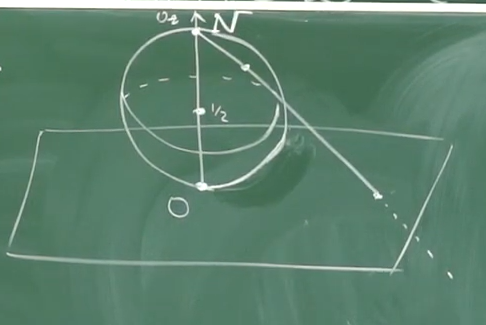
\includegraphics{assets/04-functions-of-complex-variables/stereo-graphical-projection.png}
    \end{center}

    $z = x + iy$ - плоскость. $(u, v, w) \in \mathbb{R}^3$.

    $u^2 + v^2 + (w - \frac{1}{2})^2 = \frac{1}{2^2}$

    Или же $u^2 + v^2 + w^2 = w$ - уравнение сферы Римана.
\end{definition}

\begin{theorem}
    \textbf{Связь между точкой на плоскости и точной на сфере}

    Точке $z$ соответсвует точка с координатами $(\frac{x}{1 + |z|^2}, \frac{y}{1 + |z|^2}, \frac{|z|^2}{1 + |z|^2})$

    \begin{remark}
        Точке $(u, v, w)$ соответсвует точка $z = x + iy = \frac{u}{1 - w} + i \frac{v}{1 - w}$
    \end{remark}
\end{theorem}

\begin{proof}
    Прямая через точки $(0, 0, 1)$ и $(x, y, 0)$. Параметризация луча:
    $(xt, yt, 1 - t)$. Нас интересует точка, в которой луч пересекает сферу, то есть:

    $(xt)^2 + (yt)^2 + (1- t)^2 = 1 - t$.

    $(x^2 + y^2 + 1)t^2 + 1 - 2t = 1 - t \Leftrightarrow t = \frac{1}{x^2 + y^2 + 1} = \frac{1}{|z|^2 + 1}$
\end{proof}

\begin{consequence}
    \begin{enumerate}
        \item Расстояние между образами $z$ и $\tilde{z}$ равно $\rho = \frac{|z - \tilde{z}|}{\sqrt{1 + |z|^2} \cdot \sqrt{1 + |\tilde{z}|^2}}$,
        а расстояние между $z$ и $\infty$ равно $\frac{1}{\sqrt{1 + |z|^2}}$

        \textbf{Доказательство:} предложено посчитать самому, у кого есть силы добавьте, плиз.
        
        \item Сходимость на плоскости и сходимость на сфере Римана совпадают
        
        \textbf{Доказательство:} $z_n \to z_0 \Rightarrow \frac{|z_n - z_0|}{\sqrt{1 + |z_n|^2}\cdot \sqrt{1 + |z_0|^2}} \to 0$

        $z_n \to \infty \Leftrightarrow \frac{1}{\sqrt{1 + |z_n|^2}} \to 0$

        Пусть $\frac{|z_n - z_0|}{\sqrt{1 + |z_n|^2}\cdot \sqrt{1 + |z_0|^2}} \to 0$

        Тогда $\frac{|z_n - z_0|}{\sqrt{1 + |z_n|^2}} \to 0$. Если $z_n$  ограничена, то $|z_n - z_0| \to 0$

        Если не ограничена, то возьмём $|z_{n_k}| \to \infty$, тогда $\frac{|z_{n_k} - z_0|}{\sqrt{1 + |z_{n_k}|^2}} \to 1$

        \item $\mathbb{C} \cup \{ \infty \}$ - компакт.
    \end{enumerate}
\end{consequence}

\Subsection{Вычеты}

\begin{definition}
    $a$ - изолированная особая точка. $f \in H(0 < |z - a| < R)$. 
    $f(z) = \sum_{n = -\infty}^{+\infty} c_n (z - a)^n$ - сходится при $0 < |z - a| < R$.

    $\res_{z = a} f = c_{-1}$
\end{definition}

\begin{definition}
    $f \in H(|z| > R)$ раскладывается в $f(z) = \sum_{n = -\infty}^{+\infty} c_n z^n$

    $\res_{z = \infty} f(z) = -c_{-1}$
\end{definition}

\begin{properties}
    \begin{enumerate}
        \item $f \in H(0 < |z - a| < R)$ и $0 < r < R$.
        
        Тогда $\res_{z = a} f = \frac{1}{2\pi i} \int_{|z - a| = r} f(z) \, dz$ - положительный обход
        точки $a$.

        \textbf{Доказательство:} смотреть формулу для коэффициентов ряда Лорана.

        \item $f \in H(|z| > R), r > R$.
        
        Тогда $\res_{z = \infty} f = -\frac{1}{2\pi i} \int_{|z| = r} f(z) \, dz = \frac{1}{2\pi i} \int_{|z| = r} f(z) \, dz$ - 
        положительный обход для $\infty$

        \item Если $a \in \mathbb{C}$ - полюс $n$-го порядка. 
        
        Тогда $\res_{z = a} f(z) = \lim_{z \to a} \frac{1}{(n - 1)!} \frac{d^{n - 1}}{dz^{n - 1}} ((z - a)^n f(z))$

        \textbf{Доказательство:} Считаем, что $a = 0$.

        $f(z) = \sum_{k = -n}^{+\infty} c_kz^k \Rightarrow g(z) = z^n f(z) = \sum_{k = 0}^{\infty} c_{k - n}z^k $ - формула Тейлора.

        Тогда $c_{-1} = \frac{g^{(n - 1)}(0)}{(n - 1)!}$.
        
        \item Если $a \in \mathbb{C}$ - полюс первого порядка.
        
        Тогда $\res_{z = a} f(z) = \lim_{z \to a} (z - a)f(z)$

        \item Если $a \in \mathbb{C}$, $g$ и $h$ голоморфны в окрестности точки $a$.
        $h(a) = 0, h'(a) \neq 0, g(a) \neq 0$. $f(z) = \frac{g(z)}{h(z)}$

        Тогда $\res_{z = a} f(z) = \frac{g(a)}{h'(a)}$

        \textbf{Доказательство:} $\res_{z = a} f(z) = \lim_{z \to a} (z - a)f(z) = 
        \lim_{z \to a} \frac{z - a}{h(z) - h(a)} g(z) = \frac{g(a)}{h'(a)}$

        \item Если $\lim_{z \to \infty} f(z) = A \in \mathbb{C}$.
        
        Тогда $\res_{z = \infty} f(z) = \lim_{z \to \infty} z (A - f(z))$

        \textbf{Доказательство:} $f(z) = A + \sum_{k = -\infty}^{-1} c_nz^n$, правильная часть - константа,
        иначе всё бы пошло на бесконечность. 

        \item $\res_{z = \infty} f(z) = -\res_{z = 0} \frac{f(\frac{1}{z})}{z^2}$
        
        \textbf{Доказательство:} $f(z) = \sum_{n = -\infty}^{\infty} c_nz^n$

        $\frac{1}{z^2} f(\frac{1}{z}) = \frac{1}{z^2} \sum_{n = -\infty}^{\infty} c_nz^{-n} =
        \sum_{n = -\infty}^{\infty} c_nz^{-n - 2}$
    \end{enumerate}
\end{properties}

\begin{theorem}
    \textbf{Коши о вычетах}

    $f$ голоморфна в $\Omega$, за исключением точек $a_1, \ldots a_n$.
    $K \subset \Omega$ - компакт и $a_1 \ldots a_n \in Int K$

    Тогда $\int_{\partial K} f(z) \, dz = 2\pi i \sum_{k = 1}^n \res_{z = a_k} f(z)$ 
\end{theorem}

\begin{proof}

    У каждой точки можем взять окрестность, чтобы они лежали внутри компакта и
    попарно не пересекаются. $\widetilde{K} = K \setminus \bigcup_{k = 1}^n B_{\varepsilon} (a_k)$ - компакт.
    
    А ещё $f \in H(\Omega \setminus \{ a_1 \ldots a_n\} )$

    Из интегральной формулы Коши: $\int_{\partial \widetilde{K}} f(z) \, dz = 0$

    Но $\int_{\partial \widetilde{K}} f(z) \, dz = \int_{\partial K} f(z) \, dz - \sum_{k = 1}^n \int_{|z - a_k| = \varepsilon} f(z) \, dz$, а 
    под знаком суммы - вычеты.

    
    \begin{center}
        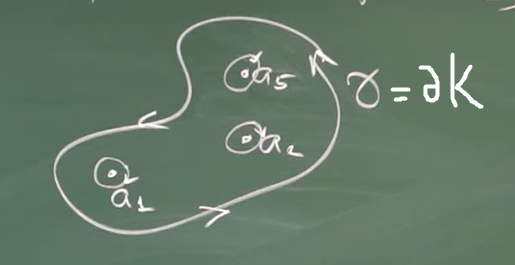
\includegraphics{assets/04-functions-of-complex-variables/koshi-theorem-for-deductions.png}
    \end{center}
\end{proof}

\begin{consequence}
    Если $f$ голоморфна в $\mathbb{C} \setminus \{ a_1 \ldots a_n \} $, то
    $\res_{z = \infty} f(z) + \sum_{k = 1}^n \res_{z = a_k} f(z) = 0$

    \textbf{Доказательство:} возьмём круг $B_R (0)$, внутри которого содержатся все эти точки.

    $\int_{|z| = R} f(z) \, dz = 2 \pi i \sum_{j = 1}^n \res_{z = a_j} f(z)$.

    Но также $\int_{|z| = R} f(z) \, dz = \int_{|z| = R}{ \sum_{k = -\infty}^{\infty} c_k z^k dz } = -2 \pi i \res_{z = \infty} f(z)$. Перекидываем и доказываем.
\end{consequence}

\begin{example}
    \begin{enumerate}
        \item {
            $\int_{|z| = 4} \frac{z^4}{e^z + 1} \, dz = 2 \pi i (\res_{z = \pi i} + \res_{z = -\pi i}) = -4\pi^5 i$.
            
            Особые точки: $e^z = -1$ при $z = \pi i + 2 \pi i k$. 

            $\res_{z = \pi i} = \frac{g(\pi i)}{h'(\pi i)} = -\pi^4$

            $g(z) = z^4, h(z) = e^z + 1$.

            $\res_{z = -\pi i} = \frac{g(-\pi i)}{h'(-\pi i)} = -\pi^4$
        }
        \item {     
            $\int_{-\infty}^{\infty} \frac{dx}{1 + x^{2n}} = \lim_{R \to +\infty} \int_{-R}^{R} \frac{dx}{1 + x^{2n}}$.
            
            \begin{center}
                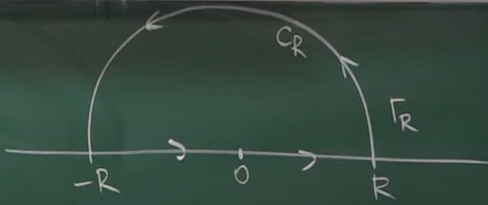
\includegraphics[width=12cm]{assets/04-functions-of-complex-variables/example-2-cauchy-about-deductions.png}
            \end{center}

            Контур - полукруг. $\int_{\Gamma_R} \frac{dz}{1 + z^{2n}} = 2 \pi i \sum \res$

            Но с другой стороны $\int_{\Gamma_R} = \int_{-R}^R + \int_{c_R}$

            $| \int_{c_R} \frac{dz}{1 + z^{2n}}| \leqslant \underbrace{\pi R}_{\text{длина кривой}} \cdot \underbrace{\max \left|\frac{1}{1 + z^{2n}}\right|}_{\text{макс. подъинтегрального выражения}} = \pi R \frac{1}{\min |1 + z^{2n}|}
            \leqslant \frac{\pi R}{R^{2n} - 1} \rightarrow 0$

            Оценка: $|a + b| \geqslant |a| - |b|$.

            Значит то, что мы хотим найти - просто сумма вычетов.

            Какие особые точки? $z^{2n} = -1$. $e^{\frac{\pi i k}{2n}}$ и $k$ нечётно.
            Нас интересует $k = 1, 3 \ldots 2n - 1$

            Тогда $I = 2 \pi i \sum_{k = 1}^n \res_{2k - 1}$

            $\res_{a_k} f = \frac{1}{(z^{2n} + 1)'} = \frac{1}{2n \cdot a_k^{2n - 1}} = \frac{a_k}{2na_k^{2n}} = -\frac{a_k}{2n}$, так как $a_k$ - полюс первого порядка. 
        }
        \item {
            Оптимизация решения из предыдущего пункта.

            $\int_{-\infty}^{+\infty} \frac{dx}{1 + x^{2n}} = 2\int_{0}^{+\infty} \frac{dx}{1 + x^{2n}} = I$

            \begin{center}
                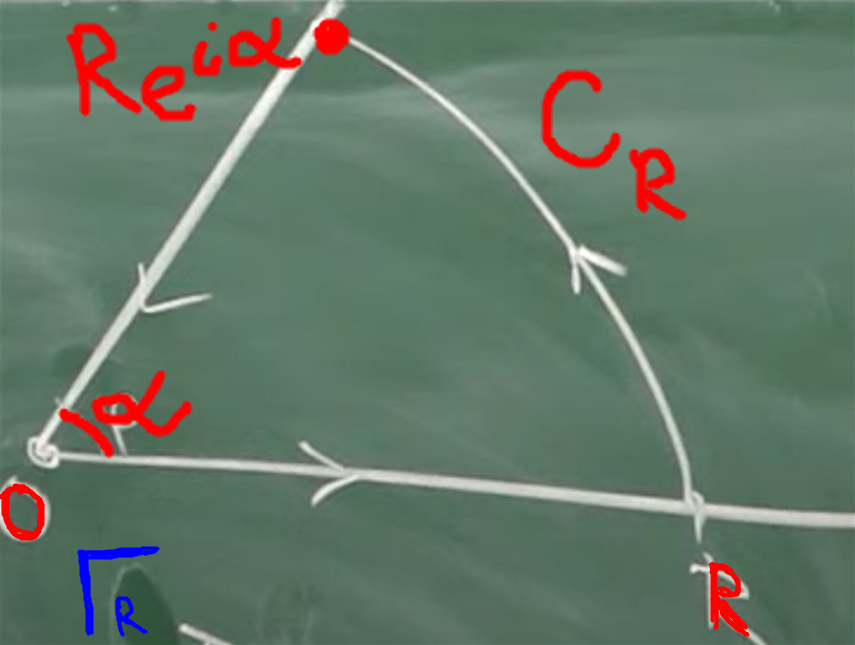
\includegraphics[width=12cm]{assets/04-functions-of-complex-variables/example-3-cauchy-about-deductions.png}
            \end{center}

            $f(x) = \frac{1}{1 + z^{2n}}$. $\int_{\Gamma_r} f(z) \, dz = \int_{c_R} + \int_{0}^{R} + \int_{Re^{i\alpha}}^{0}$.
            
            $\int_{e^{i\alpha R}}^{0} f(z) \, dz = -\int_{0}^{e^{i \alpha R}} = -\int_{0}^{R} f(e^{i \alpha} t) e^{i \alpha} \, dt$ - 
            взяли параметризацию $t \to e^{i \alpha} t$.

            $f(e^{i \alpha}t) = \frac{1}{1 + e^{2 \pi i \alpha} \cdot t^{2n}} = \frac{1}{1 + t^{2n}}$, $\alpha = \frac{\pi}{n}$.

            Единственная особая точка $e^{\frac{i \pi}{2n}}$ и интеграл равен
            $2 \pi i \res$.

            То есть: $I - e^{i \frac{\pi }{n}} I = 2 \pi i \res_{z = e^{\frac{i \pi}{2n}}} f = 2 \pi i \cdot \left ( - \frac{e^{\frac{i \pi}{2n}}}{2n}  \right )$
            
            Тогда $I = \frac{2 i e^{\frac{i \pi}{2n}}}{e^{\frac{i \pi}{2n}}} \cdot \frac{\pi}{2n} = \frac{\pi}{2n \cdot \sin \frac{\pi}{2n}}$
        }
    \end{enumerate}
\end{example}

\begin{lemma}
    \textbf{Жордана}

    $C_{R_n} = \{ z \in \mathbb{C} : |z| = R_n, \Im z \geqslant 0 \}$

    $f : \{ \Im z \geqslant 0 \} \to \mathbb{C}$. $M_{R_n} = \lim_{n \to \infty} \sup_{z \in C_{R_n}} |f(z)| = 0$

    Тогда $\forall \, \lambda > 0 \, : \, \lim \int_{C_{R_n}} f(z) e^{i \lambda z} \, dz = 0$
\end{lemma}

\begin{proof}
    Параметризация $z = R_n \cdot e^{it}$, где $t \in [0, \pi]$. 
    
    Тогда $dz = R_n e^{it} dt$.
    $\int_{C_{R_n}} f(z) e^{i \lambda z} \, dz = R_n \int_{0}^{\pi} f(R_n e^{it}) e^{it} \cdot e^{i \lambda R_n e^{it}} \, dt = I_n$

    $|I_n| \leqslant  R_n \int_{0}^{\pi} |f(R_n e^{it}) e^{it}| \cdot |e^{i \lambda R_n e^{it}}| \, dt \leqslant R_n \cdot M_{R_n} \cdot \int_{0}^{\pi} e^{- \lambda R_n \sin t} \, dt = (*) $

    То что написано под интегралом симметрично относительно $\frac{\pi}{2}$.

    $(*) = 2R_n M_{R_n} \int_{0}^{\frac{\pi}{2}} e^{-\lambda R_n \sin t} \, dt \underbrace{\leqslant}_{(**)} 
    2R_n M_{R_n} \int_{0}^{\frac{\pi}{2}} e^{-\lambda R_n \frac{2t}{\pi}} \, dt = 2R_n M_{R_n} \frac{e^{-\lambda R_n \cdot \frac{2t}{\pi}}}{-\lambda R_n \frac{2}{\pi}} \bigg |_{t = 0}^{t = \frac{\pi}{2}} 
    \leqslant M_{R_n} \cdot \frac{1}{\frac{\lambda}{\pi}} \rightarrow 0$
    
    $(**): $ верно, так как при $0 \leq t \leq \frac{\pi}{2}: \ \sin(t) \geq \frac{2}{\pi} t$
\end{proof}

\begin{example}
    $\int_0^{+\infty} \frac{\cos x}{1 + x^2} \, dx = I$.

    Можем считать на всей прямой и не исходный интеграл, а $\int_{-\infty}^{+\infty} \frac{e^{ix}}{1 + x^2} = I^*$.

    Тогда $\Re I^* = 2I$.

    Пусть $f(z) = \frac{e^{iz}}{1 + z^2}$. Контур - полуокружность от $-R$ до $R$.

    $\int_{\Gamma_R} f(z) \, dz = \int_{-R}^{R} + \int_{C_R}$. Здесь $\int_{C_R} \rightarrow 0$ по лемме
    Жордана, где $\lambda = 1$ и $M_R = \sup_{|z| = R} \left | \frac{1}{1 + z^2} \right | \leqslant \frac{1}{R^2 - 1} \rightarrow 0$

    (написанное выше верно, так как $|1 + z^2| \geqslant |z^2| - 1 = R^2 - 1$)

    Тогда $\int_{\Gamma_R} f(z) \, dz = 2 \pi i \sum \res = 2 \pi i \cdot \res_{z = i} = (*)$.

    $i$ - полюс 1 порядка, тогда $f(z) = \frac{g(z)}{h(z)}$, где $g(i) \neq 0, h(i) = 0, h'(i) \neq 0$. $
    \res = \frac{g(i)}{h'(i)} = \frac{e^{-1}}{2i}$.

    Тогда $(*) = \frac{\pi}{e}$. А значит $I = \frac{\pi}{2e}$
    
\end{example}

\begin{lemma}
    \textbf{О полувычете}

    $f \in H(0 < |z - a| < R)$ и $a$ - полюс первого порядка. $C_{\varepsilon} = \{ z \in \mathbb{C} : |z - a| = \varepsilon, \alpha \leqslant \arg (z - a) \leqslant b \}$

    \begin{center}
        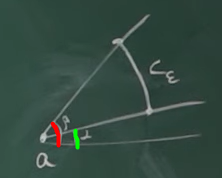
\includegraphics[width=9cm]{assets/04-functions-of-complex-variables/lemma-about-half-deduction.png}
    \end{center}

    Тогда $\lim_{\varepsilon \to 0+} \int_{C_{\varepsilon}} f(z) \, dz = (\beta - \alpha) i \cdot \res_{z = a} f$
\end{lemma}

\begin{proof}
    Считаем, что $a = 0$. У нас полюс 1-го порядка, тогда $f(z) = \frac{c}{z} + g(z)$, где $g \in H(|z| < R)$.

    Параметризация $z = \varepsilon e^{it}$, где $t \in [\alpha, \beta]$. Тогда $dz = \varepsilon e^{it} i \, dt$.

    $\int_{C_{\varepsilon}} f(z) \, dz = \int_{C_{\varepsilon}} \frac{c}{z} \, dz + \int_{C_{\varepsilon}} g(z) \, dz = 
    \int_{\alpha}^{\beta} \frac{c}{\varepsilon e^{it}} \cdot \varepsilon e^{it} i \, dt + \int_{C_{\varepsilon}} g(z) \, dz = (\beta - \alpha) \cdot i \cdot c + \int_{C_{\varepsilon}} g(z) \, dz$

    Оценим второй интеграл: $\int_{C_{\varepsilon}} g(z) \, dz \leqslant M \varepsilon (\beta - \alpha)$, где $M = \max_{|z| \leqslant \frac{R}{2}} |g(z)|$. и
    тогда $\int_{C_{\varepsilon}} g(z) \, dz \rightarrow 0$.
\end{proof}

\begin{definition}
    \textbf{Главное значение интеграла} ($v.p. \int$).

    $\int_{a}^{b} f(x) \, dx$, где $c$ - единственная особая (в этой точке нет непрерывности функции) точка, $c \in (a, b)$. 

    $\int_{a}^{c - \varepsilon} f(x) \, dx + \int_{c + \varepsilon}^{b} f(x) \, dx$ 
    и устремляем $\varepsilon$ к нулю. Предел - главное значение интеграла.
\end{definition}

\begin{example}
    $v.p. \int_{-1}^{1} \frac{dx}{x} = 0$. 

    $\lim_{\varepsilon \rightarrow 0+} \int_{-1}^{-\varepsilon} + \int_{\varepsilon}^{1} = 0$, потому что
    фукнция нечетная.

    $v.p. \int_{-\infty}^{\infty} \frac{dx}{x} = 0$
\end{example}

\begin{properties}
    \begin{enumerate}
        \item {
            Если $\int$ сходится, то $\int = v.p. \int$
        }
        \item {
            Линейность 
        }
        \item {
            Аддитивность, если резать не по особым точкам
        }
    \end{enumerate}
\end{properties}

\begin{example}
    $I = \int_{0}^{+\infty} \frac{\sin x}{x} \, dx$

    Функция четная, поэтому $2I = \int_{-\infty}^{+\infty} \frac{\sin x}{x} \, dx = v.p. \int_{-\infty}^{+\infty} \frac{\sin x}{x} \, dx$
    
    ($\frac{e^{ix}}{x} = \frac{1}{x} + \frac{ix}{x} + \ldots$).

    Тогда $2I = \Im v.p. \int_{-\infty}^{+\infty} \frac{e^{ix}}{x} \, dx$

    $v.p. \int_{-\infty}^{+\infty} = \lim_{\varepsilon \to 0, R \to +\infty} \int_{-R}^{-\varepsilon} + \int_{\varepsilon}^{R}$.

    \begin{center}
        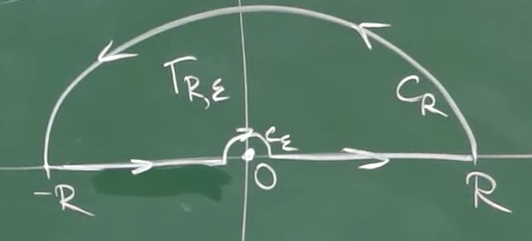
\includegraphics[width=12cm]{assets/04-functions-of-complex-variables/example-principal-value-integral.png}
    \end{center}

    $f(z) = \frac{e^{iz}}{z}$

    $\int_{\Gamma_{R, \varepsilon}} f(z) \, dz = 0$, так как особая точка только 0, а он не в контуре.
    Но с другой стороны: $\int_{\Gamma_{R, \varepsilon}} f(z) \, dz = \int_{-R}^{\varepsilon} + \int_{\varepsilon}^{R} + \int_{C_R} + \int_{C_{\varepsilon}}$

    $\int_{C_R} \rightarrow 0$ по лемме Жордана.

    $\int_{C_{\varepsilon}} f(z) \, dz \rightarrow -\pi i \res_{z = 0} f = -\pi i$.

    А значит $v.p. \int_{-\infty}^{\infty} \frac{e^{ix}}{x} \, dx = \pi i$. А значит
    $I = \frac{1}{2} \Im \ldots = \frac{\pi}{2}$
\end{example}

\newpage

\begin{example}
    $I = \int_{0}^{+\infty} \frac{x^{p - 1}}{1 + x} \, dx $, где $0 < p < 1$.
    
    \begin{center}
        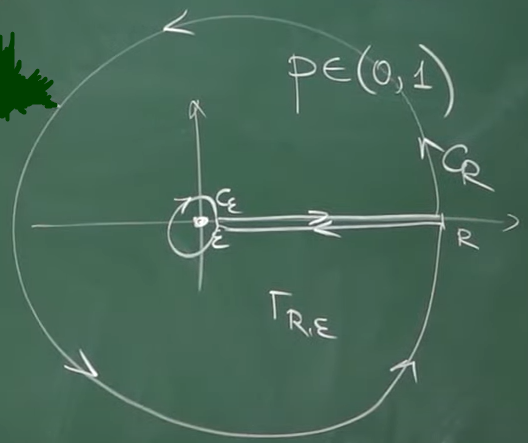
\includegraphics[width=9cm]{assets/04-functions-of-complex-variables/example-2-principal-value-integral.png}
    \end{center}

    $f(z) = \frac{e^{(p - 1) Ln z}}{1 + z}$

    $\int_{\Gamma_{R, \varepsilon}} f(z) \, dz = \int_{\varepsilon}^{R} + \int_{Re^{2\pi i}}^{\varepsilon e^{2\pi i}} + \int_{C_{\varepsilon}} + \int_{C_R}$.

    Но с другой стороны $\int_{\Gamma_{R, \varepsilon}} f(z) \, dz = 2 \pi i \sum \res = 2 \pi i \res_{z = -1}$

    $\res_{z = -1} = e^{(p - 1) Ln (-1)} = e^{(p - 1)\pi i}$

    \begin{enumerate}
        \item $\int_{\varepsilon}^{R} \rightarrow I$
        \item $\int_{Re^{2\pi i}}^{\varepsilon e^{2 \pi i}} \rightarrow -e^{(p - 1) \pi i} \cdot I$
        \item {
            $\left | \int_{C_{R}} \frac{e^{(p - 1)Ln z}}{1 + z} \, dz \right | \leqslant \pi R \cdot \max \left | \frac{e^{(p - 1) Ln z}}{1 + z} \right | = 
            \pi R \cdot \frac{R^{p - 1}}{\min |1 + z|} = \pi R \cdot \frac{R^{p - 1}}{R - 1} \rightarrow 0$

        }
        \item {
            $\left | \int_{C_{\varepsilon}} \frac{e^{(p - 1)Ln z}}{1 + z} \, dz \right | \leqslant \pi \varepsilon \cdot \max \left | \frac{e^{(p - 1) Ln z}}{1 + z} \right | = 
            \pi \varepsilon \cdot \frac{\varepsilon^{p - 1}}{\min |1 + z|} = \pi \varepsilon \cdot \frac{\varepsilon^{p - 1}}{1 - \varepsilon} \rightarrow 0$
        }

        Получили в итоге $I = \pi \frac{2i e^{(p - 1)\pi i}}{1 - e^{(p - 1)2\pi i}} = \frac{\pi}{\sin \pi p}$
    \end{enumerate}
\end{example}

\begin{theorem}

    Пусть $f$ - мероморфная функция в $\mathbb{C}$. $z_1, \ldots, z_n$ - полюсы.
    $G_1, \ldots, G_n$ - главные части рядов Лорана в точках $z_1, \ldots, z_n$.
    $\infty$ - полюс или устранимая особая точка. $G$ - правильная часть
    ряда Лорана в $\infty$

    Тогда $f(z) = G(z) + \sum_{k = 1}^n G_k(z) + C$, в частности, 
    $f$ - рациональная функция.
\end{theorem}

\begin{proof}
    $g(z) = f(z) - G(z) - \sum_{k = 1}^n G_k(z)$. У этой функции $z_1, \ldots, z_n, \infty$ - 
    устранимые особые точки, а во всех остальных точках есть голоморфность. 

    Тогда по теореме Луивилля $g \equiv const$.
\end{proof}

\begin{theorem}
    Пусть $f$ мероморфная функция в $\mathbb{C}$, $z_1, z_2 \ldots$ -- полюсы,
    $R_1, R_2, \ldots$ -- последовательность радиусов, $M_{R_n} = \max_{|z| = R_n} |f(z)| \rightarrow 0$.

    Тогда $f(z) = \lim_{n \to \infty} \sum_{k:|z_k| < R_n} G_k (z)$.
\end{theorem}

\begin{proof}
    $I_n(z) := \frac{1}{2\pi i}\int_{|\zeta| = R_n} {\underbrace{\frac{f(\zeta)}{\zeta - z}}_{=: g(\zeta)} d\zeta} = \sum res \ g = res_{\zeta = z} \ g(\zeta) + \sum_{k : \ |z_k| < R_n} res_{\zeta = z_k} \ g$

    \begin{enumerate}
        \item {
            $res_{\zeta = z} \ g = \frac{f(\zeta)}{(\zeta - z)'}|_{\zeta = z} = f(z)$ -- формула для полюса $1$-ого порядка.
        }
        \item {
            $res_{\zeta = z_k} \ g = \underbrace{res_{\zeta = z_k} \ \frac{f(\zeta) - G_k(\zeta)}{\zeta - z}}_{\text{голоморфна в окр. } z_k, т.е. равна 0} + res_{\zeta = z_k} \ \frac{G_k(\zeta)}{\zeta - z}$

            Рассмотрим окр. радиуса $R$ и запишем интеграл $\frac{1}{2 \pi i} \int_{|\zeta| = R} {\frac{G_k(\zeta)}{\zeta - z} d\zeta} = res_{\zeta = z} \ \frac{G_k(\zeta)}{\zeta - z} + res_{\zeta = z_k} \ \frac{G_k(\zeta)}{\zeta - z}$ -- так как все особые точки для подъинтегрального выражения это $z$ и $z_k$.


            $res_{\zeta = z} \ \frac{G_k(\zeta)}{\zeta - z} = G_k(z)$, а второе слагаемое равно тому, что мы хотим найти.

            $\left| \int_{|\zeta| = R} {\frac{G_k(\zeta)}{\zeta - z} d\zeta} \right| \leq 2\pi R \cdot \frac{O\left(\frac{1}{R}\right)}{R - |z|} \rightarrow 0$, где $G_k = \frac{c_{-1}}{\zeta - z_k} + \frac{c_{-2}}{(\zeta - z_k)^2} + \ldots = O(\frac{1}{R})$.

            Из стремления к нулю, мы поняли, что $res_{\zeta = z_k} \ \frac{G_k(\zeta)}{\zeta - z} = -G_k(z)$.
        }
    \end{enumerate}

    
    Теперь мы имеем, что $I_n(z) = f(z) - \sum_{k: \ |z_k| < R_n} G_k(z)$, осталось доказать, что $\lim_{n \rightarrow \infty} I_n(z) = 0$.

    $\left| I_n(z) \right| \leq \frac{1}{2 \pi} \cdot 2\pi R_n \cdot max_{|\zeta| = R_n} \left| \frac{f(\zeta)}{\zeta - z} \right| \leq R_n \cdot \frac{M_{R_n}}{R_n - |z|} \rightarrow 0$.

    % $\frac{1}{2\pi i} \int_{|\zeta| = R_n} \frac{f(\zeta)}{\zeta - z} \, d \zeta = \sum \res \frac{f(\zeta)}{\zeta - z} = (*)$

    % $\left| \frac{1}{2\pi i} \int_{|\zeta| = R_n} \frac{f(\zeta)}{\zeta - z} \, d \zeta \right| = R_n \cdot 
    % \max_{|\zeta| = R_n} \left | \frac{f(\zeta)}{\zeta - z} \right | \leqslant R_n \cdot \frac{M_{R_n}}{R_n - |z|} \rightarrow 0$

    % Какие особые точки есть у $(*)$ -- особые точки $z$ и особые точки $f$. 
    % Поймём, как устроены вычеты в этих особых точках.

    % \begin{enumerate}
    %     \item {
    %         $\res_{\zeta = z} \frac{f(\zeta)}{\zeta - k}$ - полюс первого порядка, значит:
            
    %         $\res_{\zeta = z} \frac{f(\zeta)}{\zeta - k} = f(z)$
    %     }
    %     \item {
    %         $\res_{\zeta = z_k} \frac{f(\zeta)}{\zeta - z} = \res_{\zeta = z_k} \frac{G_k (\zeta)}{\zeta - z}$, так как разность -- голоморфная в точке $z_k$ функция. 

    %         Такой вычет посчитаем так, посчитаем интеграл по кружности радиуса $R$:

    %         $\frac{1}{2\pi i} \int_{|\zeta| = R} \frac{G_k (\zeta)}{\zeta - z} \, d\zeta = \res_{\zeta = z} + \res_{\zeta = z_k}$.
            
    %         С другой стороны:

    %         $\left | \frac{1}{2\pi i} \int_{|\zeta| = R} \frac{G_k (\zeta)}{\zeta - z} \, d\zeta \right | \leqslant R \cdot \frac{\max_{|\zeta| = R} |G_k (\zeta)|}{R - |z|} \rightarrow 0$.
            
    %         А значит $-\res_{\zeta = z} = \res_{\zeta = z_k}$.

    %         Отсюда получили, что $\res_{\zeta = z_k} \frac{G_k (\zeta)}{\zeta - z} = \res_{\zeta = z} \frac{G_k(\zeta)}{\zeta - z} = -G_k (z)$.
    %     }
    % \end{enumerate}
    % Тогда $(*) = f(z) - \sum_{k : |z_k| < R_n} G_k (z)$.
\end{proof}

% \begin{example}
%     $f(z) = \frac{\ctg z}{z}$. Особые точки вида $\pi k, k \in \mathbb{Z}$. Давайте брать $R_n = \pi n + \frac{\pi}{2}$.

%     % Тут, наверное, нужна картинка. 

%     \begin{lemma}
        % Существует $M$, такая что, $|\ctg z| \leqslant M$ при $|z| = \pi (n + \frac{1}{2})$.
%     \end{lemma}

%     $M_{R_n} \leqslant \frac{M}{R_n} \rightarrow 0$. Тогда исходя из теоремы 
%     $\frac{\ctg z}{z} = \lim_{n \to \infty} \sum_{-n}^n G_k(z)$, где $G_k$ - главная часть ряда Лорана в точке 
%     $\pi k$.

%     Пусть $k \neq 0$, тогда $f$ имеет в точке $\pi k$ полюс первого порядка. 
%     Тогда $G_k(z) = \frac{\res}{z - \pi k}$.

%     Нас интересует $\res_{z = \pi k} \frac{\ctg z}{z} = \res_{z = \pi k} \frac{\frac{\cos z}{z}}{\sin z}$.
%     Числитель и знаменатель голоморфны и $z = \pi k$ - ноль первой кратности. Тогда
%     $\res = \frac{\frac{\cos z}{z}}{(\sin z)'} = \frac{1}{\pi k}$.

%     Поэтому $G_k(z) = \frac{1}{\pi k(z - \pi k)}$

%     $z = 0$. Интересуемся $G_0(z) = \frac{a}{z} + \frac{b}{z^2}$. Здесь $a = 0$, так как функция чётная, $b = 
%     \res_{z = 0} \ctg z = \res_{z = 0} \frac{\cos z}{\sin z} = 1$.

%     То есть $\frac{\ctg z}{z} = \frac{1}{z^2} \lim_{n \to \infty} \sum_{k = 1}^n \left ( \frac{1}{\pi k(z - \pi k)} - \frac{1}{\pi k(z + \pi k)} \right ) =
%     \frac{1}{z^2} + \sum_{k = 1}^{\infty} \frac{2}{z^2 - \pi^2 k^2}$

%     \begin{proof}
%         \textbf{леммы про $\ctg$}

%         Нужен рисунок, без него беда. Тут потеряно доказательство.
%         %Рисунок и пруф.
%     \end{proof}
% \end{example}

\begin{example}
    $\ctg(z) = \frac{1}{z} + \sum_{k=1}^{\infty} \frac{2z}{z^2 - \pi^2 k^2}$
\end{example}

\begin{lemma}
    Существует $M$, такая что, $|\ctg z| \leqslant M$ на окружностях $|z| = \pi (n + \frac{1}{2})$, где $n \in \mathbb{N}$.
\end{lemma}
\begin{proof}
    Леммы.

    Наблюдения про $\ctg z$:
    \begin{enumerate}
        \item $\pi$-периодическая функция $\implies$ все значения содержатся в полосе $0 \leq Re(z) \leq \pi$, можно все окружности сдвинуть по периоду.
        \item нечетная функция $\implies$ можем интересоваться только половиной картинки (давайте смотреть на $Re(z) \geq 0$).
    \end{enumerate}

    \begin{center}
        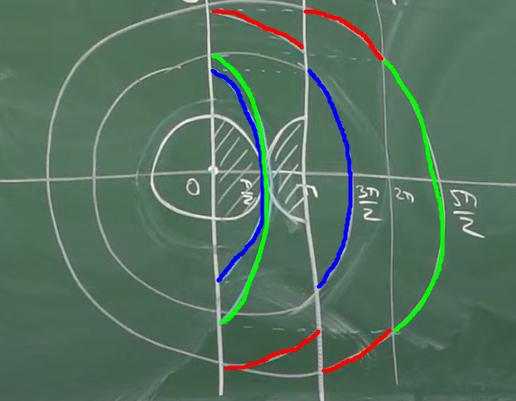
\includegraphics[width=9cm]{assets/04-functions-of-complex-variables/ctg-lemma.png}
    \end{center}

    Мы получаем полосу, за некоторым исключением (так как есть определенные точки, которые точно не получаются):

    $\{ 0 \leq Re(z) \leq \pi \} \setminus \{ |z| < \frac{\pi}{2} \} \cup \{ |z - \pi| < \frac{\pi}{2} \}$.

    Получаем следующее мн-во:

    \begin{center}
        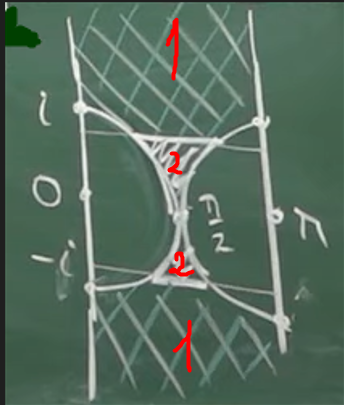
\includegraphics[height=6cm]{assets/04-functions-of-complex-variables/ctg-lemma-2.png}
    \end{center}

    Хотим понять, что $\ctg$ ограничен на заштриховоном мн-ве.

    $z = x + iy$

    \begin{enumerate}
        \item {
            Зона 1 ($y \geq 1$ или $y \leq -1$, в силу нечетности $\ctg$):

            $|\ctg z| = |\frac{\cos z}{\sin z}| = \left|\frac{e^{iz} + e^{-iz}}{e^{iz} - e^{-iz}}\right| = \left| \frac{1 + e^{2iz}}{1 - e^{2iz}} \right| \leq  \frac{1 + \left|e^{2iz}\right|}{\left|1 - e^{2iz}\right|} = (*)$

            Пусть $z = x + iy$ и пока что $y \geq 1$:
        
            $|e^{2iz}| = |e^{2ix} \cdot e^{-2y}| = e^{-2y}$, тогда $(*) = \frac{1 + e^{-2y}}{|1 - e^{2iz}|} \leq \frac{1 + e^{-2y}}{1-e^{-2y}} \leq \frac{2}{1 - e^{-2}}$ 
        }
        \item {
            Зона 2:

            Очевидно, что эта зона это компакт, а $\ctg$ на ней непрерывен $\implies$ $\ctg$ -- ограничен на этом компакте.
        }
    \end{enumerate}
\end{proof}

\begin{proof}
    Примера.

    $f(z) = \frac{\ctg z}{z}$, из леммы: $\ctg z \leq M$ при $|z| = \pi (n + \frac{1}{2})$.

    Берем радиусы $R_n = \pi (n + \frac{1}{2}) \implies M_{R_n} \leq \frac{M}{\pi (n + \frac{1}{2})} \rightarrow 0$.

    Особые точки $f(z): \ z = 0 \text{ -- полюс 2-ого порядка}, z = \pi k \text{ -- полюсы 1-ого порядка при } k \neq 0$.

    $G_k$ -- главная часть ряда Лорана в $\pi k, \ k \neq 0$ $\implies G_k(z) = \frac{res_{z = \pi k} \ \ctg(z)}{z - \pi k} = \frac{1}{\pi k(z - \pi k)}$, где $res_{z = \pi k} \ \ctg(z) = \frac{\cos(z)}{\sin'(z)} |_{z = \pi k} = \frac{1}{\pi k}$.


    $G_0(z) = \frac{A}{z^2} + \frac{res_{z = 0} \ f(z)}{z} = \frac{A}{z^2}$, вычет занулился, так как $f(z)$ -- четная функция и все коэффициенты перед нечетными степенями в ряде Лорана равны $0$.

    $G_0(z) = \frac{A}{z^2} = \frac{1}{z^2}$, так как $\frac{\ctg(z)}{z} = \frac{\cos(z)}{z \sin(z)} \sim \frac{1}{z^2}$ при $z$ близких к нулю.

    То есть $\frac{\ctg(z)}{z} = G_0(z) + \sum_{k=1}^{\infty} \left(G_{k}(z) + G_{-k}(z)\right) =$
    
    $= \frac{1}{z^2} + \sum_{k=1}^{\infty} \left( \frac{1}{\pi k(z - \pi k)} + \frac{1}{\pi (-k) (z + \pi k)} \right) = \frac{1}{z^2} + \sum_{k=1}^{\infty} \frac{2}{z^2 - \pi^2 k^2}$.
\end{proof}

\begin{example}
    $(\ln \sin z)' = \ctg z$

    $(\ln \frac{\sin z}{z})' = \ctg z - \frac{1}{z}$.

    $\ln \frac{\sin z}{z} = \int_{0}^{z} (\ctg w - \frac{1}{w}) \, dw = \int_{0}^{z} \sum_{k=1}^{\infty} \frac{2w}{w^2 - \pi^2 k^2} \, dw = 
    \sum_{k = 1}^{\infty} \int_{0}^{z} {\frac{2w}{w^2 - \pi^2 k^2} dw}$ (можем переставлять, потому что есть равномерная сходимость).
    
    $\sum_{k = 1}^{\infty} \int_{0}^{z} \left ( \frac{1}{w - \pi k} + \frac{1}{w + \pi k} \right ) =$

    $= \sum_{k = 1}^{\infty} \ln (w - \pi k) + \ln (w + \pi k) \bigg |_{0}^z = \sum_{k = 1}^{\infty} \ln 
    \left ( \frac{z^2 - \pi^2 k^2}{-\pi^2 k^2} \right ) = \sum_{k = 1}^{\infty} \ln \left ( 1 - \frac{z^2}{\pi^2 k^2} \right )$.

    Тогда $\frac{\sin z}{z} = \prod_{k = 1}^{\infty} \left(1 - \frac{z^2}{\pi^2 k^2} \right)$.
    
    Либо $\sin z = z \prod_{k = 1}^{\infty} \left(1 - \frac{z^2}{\pi^2 k^2} \right)$.
\end{example}

\begin{example}
    $\sum_{n = 1}^{\infty} \frac{1}{n^2} = \frac{\pi^2}{6}$

    $f(z) = \frac{1}{z^2}$. Посмотрим на $f(z) \cdot \ctg (\pi z)$. Тогда
    $\res_{z = k} f(z) \cdot \ctg (\pi z) = \frac{f(k)}{\pi}$.

    $g(z) = \frac{\ctg \pi z}{z^2}$ и проинтегрируем.

    $\frac{1}{2 \pi i} \int_{|z| = n + \frac{1}{2}} \frac{\ctg \pi z}{z^2} \, dz = 
    \sum_{k = -n, k \neq 0}^n \frac{1}{\pi k^2} + \res_{z = 0} \frac{\ctg \pi z}{z^2}$.

    При этом есть такая оценка:
    $\left | \frac{1}{2 \pi i} \int_{|z| = n + \frac{1}{2}} \frac{\ctg \pi z}{z^2} \, dz \right | \leqslant 
    (n + \frac{1}{2}) \cdot \frac{M}{(n + \frac{1}{2})^2} \rightarrow 0$

    Значит, $\sum_{k = 1}^{\infty} \frac{1}{k^2} = -\frac{\pi}{2} \cdot \res_{z = 0} \frac{\ctg \pi z}{z^2}$.
    
    Такой вычет не очень приятно считать -- раскладываем в ряд.

    Найдем коэффициент перед $z^1$: в разложении $\ctg \pi z = \frac{\cos \pi z}{\sin \pi z} = \frac{1 - \frac{\pi^2 z^2}{2} + \mathcal{O}(z^4)}{\pi z (1 - \frac{\pi^2 z^2}{6} + \mathcal{O}(z^4))} = $


    $ = \frac{(1 - \frac{\pi^2 z^2}{2} + \mathcal{O}(z^4))(1 + \frac{\pi^2 z^2}{6} + \mathcal{O}(z^4))}{\pi z} = \frac{1}{\pi z} - \frac{1}{3} \pi z + \mathcal{O}(z^3)$.

    То есть этот коэффициент равен: $-\frac{\pi}{3}$.

    Тогда $\sum_{k = 1}^{\infty} \frac{1}{k^2} = -\frac{\pi}{2} \cdot (-\frac{\pi}{3}) = \frac{\pi^2}{6}$.
\end{example}

\begin{theorem} (О числе нулей и полюсов).

    Пусть $f$ мероморфна в $\Omega$, $\gamma$ - простая замкнутая кривая в $\Omega$, 
    не проходящая через нули и полюсы $f$.

    Тогда $\frac{1}{2 \pi i} \int_{\gamma} \frac{f'(z)}{f(z)} \, dz = \mathcal{N}_f - \mathcal{P}_f$

    $\mathcal{N}_f$ - количество нулей $f$ с учетом кратности в контуре $\gamma$.

    $\mathcal{P}_f$ - количество полюсов $f$ с учетом кратности (порядка) в контуре $\gamma$.

    \begin{consequence}
        Если $f \in H(\Omega)$, $\gamma$ - простая замкнутая кривая, не проходящая через нули $f$, тогда
        $\frac{1}{2\pi i} \int_{\gamma} \frac{f'(z)}{f(z)} \, dz = \mathcal{N}_f$
    \end{consequence}
\end{theorem}

\begin{proof} Теоремы.

    Если $a$ - ноль или полюс $f$, то $f(z) = (z - a)^m g(z)$, где $g(a) \neq 0$ и 
    $g$ голоморфна в окрестности $a$.

    \begin{enumerate}
        \item Если $a$ - ноль, то $m$ - кратность нуля
        \item Если $a$ - полюс, то $m$ - порядок полюса.
    \end{enumerate}

    $f'(z) = m(z - a)^{m - 1} g(z) + (z - a)^m g'(z)$

    $\frac{f'(z)}{f(z)} = \frac{m}{z - a} + \frac{g'(z)}{g(z)}$, второе слагаемое голоморфно в окрестности $a$. Значит,
    $a$ - полюс первого порядка $\frac{f'}{f}$, а $m$ - вычет.
\end{proof}

\begin{consequence}
    \textbf{Принцип аргумента}

    Пусть $f \in H(\Omega)$, $\gamma$ - простая замкнутая кривая в $\Omega$, не проходящая через
    нули $f$. 
    
    Тогда $\mathcal{N}_f = \frac{1}{2\pi} \Delta_{\gamma} \arg f(z)$, где $\Delta_{\gamma}$ - изменение аргумента
    при движении по кривой.
\end{consequence}

\begin{proof}
    $\mathcal{N}_f = \frac{1}{2\pi i} \int_{\gamma} \frac{f'(z)}{f(z)} \, dz$. Но $\frac{f'}{f} = (Ln f)'$. 
    Если рассмотрим $Ln$ на кривой $\gamma$, то это будет первообразная вдоль пути $\gamma$ для $\frac{f'}{f}$.

    $\mathcal{N}_f = \frac{1}{2\pi i} \Delta_\gamma (Ln f(z)) = \frac{1}{2 \pi i} (\Delta_\gamma
    (\ln |f(z)| + i\arg f(z))) = \frac{1}{2\pi} \Delta_{\gamma} \arg f(z)$
\end{proof}

\begin{theorem}
    \textbf{Руше}

    $f, g \in H(\Omega)$, $\gamma$ - простой замкнутая кривая в $\Omega$ и 
    $|f| > |g|$ на $\gamma$.

    Тогда $f + g$ и $f$ внутри $\gamma$ имеют одинаковое число нулей с учетом кратности.
\end{theorem}

\begin{proof}
    $\mathcal{N}_{f + g} = \frac{1}{2 \pi} \Delta_\gamma \arg (f + g)$.
    $|f + g| \geqslant |f| - |g| > 0$ на $\gamma$, поэтому в ноль обращения нет и
    можно использовать принцип аргумента.

    $\mathcal{N}_{f + g} = \frac{1}{2\pi} \Delta_\gamma \arg (f \cdot (1 + \frac{g}{f})) = 
    \frac{1}{2\pi} \Delta_\gamma \arg f + \frac{1}{2\pi} \Delta_\gamma \arg (1 + \frac{g}{f})$.

    Значит надо доказать, что $\Delta_\gamma \arg (1 + \frac{g}{f}) = 0$.

    Значения $1 + \frac{g}{f}$ на $\gamma$ лежат в круге $|z - 1| < 1$, потому что $\frac{|g|}{|f|} < 1$. А значит
    вокруг нуля обойти не можем и изменения аргумента нет.
\end{proof}

\begin{example}
    $z - e^{-z} = \lambda > 1$. Хотим понять, что в правой полуплоскости есть ровно 1 корень.

    \begin{center}
        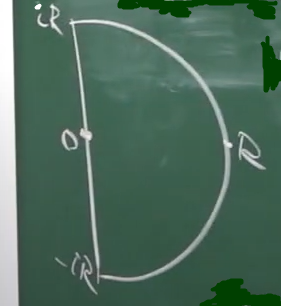
\includegraphics[width=7cm]{assets/04-functions-of-complex-variables/rushe-example.png}
    \end{center}

    Возьмём окружность большого радиуса и по ней обход по контуру $\gamma$.

    Возьмём $f(z) = z - \lambda$ и $g(z) = -e^{-z}$. Хотим подставить в т. Руше, тогда необходимо чтобы $|f| > |g|$, проверим это: 
    
    \begin{enumerate}
        \item {
            На вертикальном отрезке: $|f(z)| = |iy - \lambda| = \sqrt{y^2 + \lambda^2} \geqslant \lambda > 1$, а
            $|g(z)| = |-e^{-iy}| = 1$, значит всё выполняется.
        }
        \item {
            На полуокружности: $|f(z)| = |z - \lambda| \geqslant |z| - \lambda = R - \lambda$, а $|g(z)| = |-e^{-x - iy}| = e^{-x} \leqslant 1$. То есть если $R > \lambda + 1$, то $|f| > |g|$ на $\gamma$.
        }
    \end{enumerate}

    Тогда $\mathcal{N}_{f + g} = \mathcal{N}_f = 1$
\end{example}

\Subsection{Конфорные отображения}

\begin{definition}
    $\Omega$ и $\tilde{\Omega}$, тогда $f: \Omega \to \tilde{\Omega}$ - конфорное отображение,
    если $f$ биекция и $f \in H(\Omega)$
\end{definition}

\begin{theorem}
    Пусть $f \in H(\Omega)$, $a \in \Omega$, такая, что $f'(a) \neq 0$.
    
    Тогда $f$ сохраняет углы между кривыми, проходящими через точку $a$.  
\end{theorem}

\begin{proof}
    $\gamma : [0, 1] \to \Omega$ и $\gamma (0) = a$ (можно так считать).
    
    $\tilde{\gamma} : [0, 1] \to \Omega$ и $\tilde{\gamma} (0) = a$.

    $\arg \gamma'(0) - \arg \tilde{\gamma}'(0)$ - угол между кривым в $\Omega$.

    $\arg (f \circ \gamma)'(0) - \arg (f \circ \tilde{\gamma})'(0) = \arg f'(a)\gamma'(0) - \arg f'(a) \tilde{\gamma}'(0) = 
    \arg \tilde{\gamma}'(0) - \arg \tilde{\gamma}'(0)$
\end{proof}

\begin{definition}
    $f : \Omega \to \mathbb{C}$ - однолистная, если $f \in H(\Omega)$ и 
    инъекция.
\end{definition}

\begin{theorem}
    Если $f \in H(\Omega)$ и $f \neq const$, то $f(\Omega)$ - область.
\end{theorem}

\begin{proof}
    \begin{enumerate}
        \item {
            Линейная связность остаётся
        }
        \item {
            Нужно проверить, что $f(\Omega)$ - открытое множество. Возьмём точку 
            в образе и докажем, что она там лежит с некоторым шариком.

            $b \in f(\Omega) \Rightarrow \exists \, a \in \Omega \, : \, f(a) = b$.


            \begin{center}
                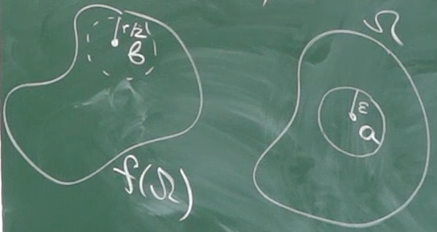
\includegraphics[width=10cm]{assets/04-functions-of-complex-variables/single-leaf-theorem.png}
            \end{center}

            Найдётся окружность $|z - a| < \varepsilon$, что $|f(z) - b| \neq 0$. Если на окружности радиуса $\frac{1}{n}$ нашлась точка $z_n$, 
            такая, что $f(z_n) = b$, то $f \equiv b$ по теореме единственности.

            $r = \min_{|z - a| = \varepsilon} |f(z) - b| > 0$. Посмотрим на $f(z) - w$. Хотим понять, что такое уравнение
            имеет решение при $w$ близких к $b$. Это и будет значить, что близкие к $b$ точки попадают в образ.

            Подставим всё в теорему Руше. $f(z) - w = (f(z) - b) + (b - w)$. Нужно, чтобы $|f(z) - b| > |b - w|$. Возьмём $|b-w| < r$ и всё выполнится.

            Получили, что $\{ |w-b| < r \} \subset f(\Omega) \Rightarrow f(\Omega)$ открытое.
        }
    \end{enumerate}
\end{proof}

\begin{consequence}
    Если $f$ однолистна, то $f$ конформное отображние $\Omega$ на $f(\Omega)$.
\end{consequence}

\begin{theorem}
    $f : \Omega \to \mathbb{C}$ однолистна. Тогда $f'(z) \neq 0 \, \forall \, z \in \Omega$.
\end{theorem}

\begin{proof}
    Пусть $f'(a) = 0$, $b = f(a)$. Возьмём $\varepsilon$ так, что
    $f(z) - b \neq 0$ при $|z - a| = \varepsilon$ и $r = \min_{|z - a| = \varepsilon} |f(z) - b| > 0$.

    \begin{center}
        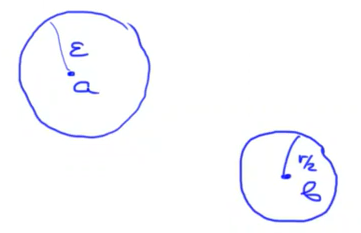
\includegraphics[width=6cm]{assets/04-functions-of-complex-variables/single-leaf-theorem-derivative-none-zero.png}
    \end{center}

    Смотрим на уравнение $f(z) - w = f(z) - b + b - w$. Мы выяснили, что 
    $\mathcal{N}_{f - w} = \mathcal{N}_{f - b} \geqslant 2$, потому что
    $a$ - корень кратности $\geqslant 2$. Тогда $f(z) = w$ имеет хотя бы 2 решения. Но у нас инъекция, поэтому
    все решения с кратностью 2. Хотим показать, что тогда найдётся последовательность нулей производных, 
    стремящаяся к точке $a$ и получить противоречие.

    Берём радиус $\frac{r}{2}$. $\{ |w - b| \leqslant \frac{r}{2} \} \subset f(\Omega)$.
    Берём $w_1, w_2, \ldots$ из этого круга. Значит $\exists \, z_1, \ldots$ из $|z - a| < \varepsilon$, 
    $f(z_k) = w_k$ и $f'(z_k) = 0 \Rightarrow$ в $|z - a| \leqslant \varepsilon$ бесконечно много нулей
    $f'$. Значит у них есть предельная точка и тогда $f' \equiv 0 \Rightarrow f \equiv const$.
\end{proof}

\begin{remark}
    Обратное неверно. $f(z) = e^z, f'(z) = e^z \neq 0$, но нет однолистности.
\end{remark}

\begin{consequence}
    \begin{enumerate}
        \item {
            Конформное отображение сохраняет углы между кривыми

            \textit{Доказательство: } оно инъективно, а значит производная в ноль не обращается.
        }
        \item {
            Если $f(z) = c_0 + \frac{c_1}{z} + \frac{c_2}{z^2} + \ldots$ однолистна
            в окрестности $\infty$, то $c_1 \neq 0$.

            \textit{Доказательство: } $g(z) = f(\frac{1}{z})$ однолистна в проколотой окрестности нуля, в нуле можем доопределить, чтобы была голоморфность.

            \begin{center}
                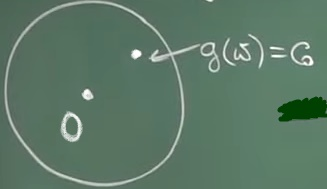
\includegraphics[width=7cm]{assets/04-functions-of-complex-variables/conf-func-consequence-2.jpg}
            \end{center}
            $g$ однолистна в меньшей не проколотой окрестности $\Rightarrow c_1 = g'(0) \neq 0$ 
        }
        \item {
            $f$ имеет полюс в точке $a$ и однолистна в проколотой окрестности точки $a$, 
            тогда это полюс первого порядка.

            \textit{Доказательство: } пусть $g(z) = \frac{1}{f(z)}$ - однолистна в проколотой окрестности точки $a$.
            Можем доопределить нулём в точке $a$ и тогда будет голоморфность, $g(a) = 0$.

            Тогда $g$ однолистна в окрестности точки $a$, а значит $g'(a) \neq 0$, тогда $a$ - 
            ноль первого порядка у $g$, а значит и ноль первого порядка у $f$.
        }
    \end{enumerate}
\end{consequence}

\begin{definition}
    $\Omega$ и $\tilde{\Omega}$ конформно эквивалентны, если $\exists \, f : \Omega \to \tilde{\Omega}$ - конформное отображение.

    \begin{remark}
        Это отношение эквивалентности.
    \end{remark}
\end{definition}

\begin{theorem}
    $\mathbb{C}$ и $\mathbb{D}$ не конформно эквивалентны.
\end{theorem}

\begin{proof}
    От противного. Пусть $f : \mathbb{C} \to \mathbb{D}$ - конформное отображение.

    Тогда $f \in H(\mathbb{C})$, $|f| \leqslant 1$. Тогда $f$ константа
    по теореме Луивилля. А это не биекция
\end{proof}

\begin{lemma}
    \textbf{Шварца}

    $f : \mathbb{D} \to \mathbb{D}$ голомофрная, $f(0) = 0$. Тогда:
    \begin{enumerate}
        \item $|f(z)| \leqslant |z| \forall \, z \in \mathbb{D}$
        \item Если для какого-то $a$, $|f(a)| = |a|$, то $f(z) = e^{i\phi} z$, где $\phi \in \mathbb{R}$
    \end{enumerate}
\end{lemma}

\begin{proof}
    \begin{enumerate}
        \item {
            Пусть $g(z) = \frac{f(z)}{z}$, в нуле устранимая особая точка, устраним - получим голоморфную в круге функцию.
            %TODO
            Согласно принципу максимума, в круге $|g(z)| \leqslant \max_{|z| = r} |g(z)| \leqslant \frac{1}{r} \rightarrow_{r \to 1-} 1$.
            И тогда $\frac{|f(z)|}{|z|} \leqslant 1$
        }
        \item {
            Знаем, что $|g(z)| \leqslant 1$ в $\mathbb{D}$. Если $|g(a)| = 1$, для $a \in \mathbb{D}$, то 
            $a$ локальный максимум модуля и тогла, по принципу максимума, $g \equiv const \Rightarrow g(z) = e^{i\phi}$
        }
    \end{enumerate}
    
\end{proof}

\begin{theorem}
    \textbf{Римана о конфорных отображениях}

    $\Omega$ и $\tilde{\Omega}$ - односвязные области в $\bar{\mathbb{C}}$, причём их
    граница состоит больше, чем из одной точки (есть хотя бы какая-то кривая).
    Есть точка $z_0 \in \Omega, \tilde{z_0} \in \tilde{\Omega}$ и $\alpha \in \mathbb{R}$.

    Тогда существует единственное конформное отображение $f : \Omega \to \tilde{\Omega}$, такое,что
    $f(z_0) = \tilde{z_0}$ и $\arg f'(z_0) = \alpha$.
\end{theorem}

\begin{proof}
    \textit{Единственность}

    \begin{enumerate}
        \item {
            $\Omega = \tilde{\Omega} = \mathbb{D}, z_0 = \tilde{z_0} = 0$.

            Пусть $f : \mathbb{D} \to \mathbb{D}$, $f(0) = 0$ и $\arg f'(0) = \alpha$.
            По лемме Шварца для $f$ получаем, что $|f(z)| \leqslant |z| \, \forall z \in \mathbb{D}$.
            
            С другой стороны, $f^{-1} : \mathbb{D} \to \mathbb{D}$ тоже конфорное, $f^{-1}(0) = 0$, значит для
            неё тоже можно применить лемму Шварца. $|f^{-1}(z)| \leqslant |z| \Rightarrow |z| \leqslant |f(z)|$.

            Значит $|f(z)| = |z| \, \forall z \in \mathbb{D}$, тогда по лемме Шварца это поворот, то есть $f(z) = e^{i\phi}z$.
            
            Также мы знаем, что $f'(z) = e^{i\phi}$ и $\arg f'(0) = 0 \implies e^{i\phi} = 1$. 
        }
        \item {
            $\Omega$ и $\tilde{\Omega}$ проивзольные. Пусть $f_1, f_2 \, : \, \Omega \to \tilde{\Omega}$ - конфорное.
            $f_i(z_0) = \tilde{z_0}$ и $\arg f_i' (z_0) = \alpha$, где $i \in \{1, 2\}$.

            Воспользуемся \textit{существованием}:
            
            \begin{enumerate}
                \item {
                    $\exists \phi : \mathbb{D} \rightarrow \Omega$ -- конформное, $\phi(0) = z_0$ и $\phi'(0) > 0$ (то есть, что $\arg \phi'(0) = 0$).
                }
                \item {
                    $\exists \psi : \tilde{\Omega} \rightarrow \mathbb{D}$ -- конформное, $\psi(\tilde{z_0}) = 0$ и $\arg \psi'(\tilde{z_0}) = -\alpha$.
                }
            \end{enumerate}

            Посмотрим на $g_i = \psi \circ f_i \circ \phi: \mathbb{D} \rightarrow \mathbb{D}$:

            \begin{enumerate}
                \item $g_i(0) = 0$
                \item {
                    $g_i'(0) = \psi'(f_i(\phi(0))) \cdot f_i'(\phi(0)) \cdot \phi'(0) = \psi'(\tilde{z_0}) \cdot f_i'(z_0) \cdot\phi'(0)$

                    $\arg g_i'(0) = -\alpha + \alpha + 0 = 0$ -- сумма аргументов множителей.
                }
            \end{enumerate}

            То есть мы получили, что $g_1$ и $g_2$ -- два комфорных отображения из круга в круг, переводящие ноль в ноль, и производную в нуле имеют с нулевым аргументом $\implies_{\text{по пункту (1)}} g_1 = g_2 = z$.

            Тогда восстановим $f_i$ и поймем, что они равны:

            $f_i(\phi(z)) = \psi^{-1}(g_i(z)) \implies f_i(z) = \psi^{-1}(g_i(\phi^{-1}(z))) \implies$ т.к. $g_1 = g_2$, то по полученной формуле $f_1 = f_2$.
        }
    \end{enumerate}
\end{proof}

\begin{consequence}
    \textbf{Обобщенная теорема Лиувилля}

    $f \in H(\mathbb{C})$ и $f$ не принимает значения на некоторой кривой $\gamma$. Тогда
    $f \equiv const$
\end{consequence}

\begin{proof}
    $\bar{\mathbb{C}} \setminus \gamma$ - односвязная область, с границей, состоящей из более чем одной точки.

    Тогда по теореме Римана о комформных отображениях существует $g : \bar{\mathbb{C}} \setminus \gamma \to \mathbb{D} \Rightarrow g \circ f \in H(\mathbb{C})$ и $g \circ f \subset \mathbb{D}$, то есть
    это ограниченная функция.

    Тогда по теореме Лиувилля (стандартной), $g \circ f$ - константа, значит
    $f(z) = g^{-1} (const) = const$.
\end{proof}

\begin{remark}
    \textbf{Малая теорема Пикара}

    Если $f \in H(\mathbb{C})$ не принимает 2 каких-то значения, то 
    $f \equiv const$.
\end{remark}

\begin{example}
    $f(z) = e^z \neq 0$ - одно значение целая функция может не принимать.
\end{example}

\begin{consequence}
    Если $f$ мероморфна в $\mathbb{C}$ и не принимает 3 значения, то $f \equiv const$
\end{consequence}

\begin{proof}
    Пусть нет значений $a, b, c$. Сделаем из меромофрной - голоморфную, которая не принимает 2 значения.
    Пусть $c \neq \infty$, тогда $g(z) = \frac{1}{f(z) - c} \in H(\mathbb{C})$, но она не
    принимает значения $\frac{1}{a - c}$ и $\frac{1}{b - c}$, а тогда по малой теореме Пикара получаем, что $f \equiv const$.
\end{proof}

\begin{example}
    $f(z) = \tg z \neq \pm i$ - пример мероморфной функции, не принимающей 2 значения.
\end{example}

\begin{definition}
    $f(z) = \frac{az + b}{cz + d}$ - дробно-линейное отображение, $ad - bc \neq 0$.
\end{definition}

\begin{theorem}
    Если $f \in H(\bar{\mathbb{C}} \setminus \{z_0\})$ и однолистна, то $f$ дробно-линейное отображение.
\end{theorem}

\begin{proof}
    % $z_0$ - изолированная особая точка. 

    \begin{enumerate}
        \item {
            $z_0$ -- существенная особая точка. Тогда по теореме Сохоцкого 
            $Cl \, f \{ 0 < |z - z_0| < \varepsilon \} = \mathbb{C}$.

            Возьмём $b = f(a)$. Тогда $f(|z - a| < r)$ - открытое множество (т.к. $\{|z-a| < r\}$ -- открытое и $f$ -- однолистная).
            
            Более того, $f(|z - a| < r) \cap f(0 < |z - z_0| < \varepsilon) = \emptyset$ из однолистности.


            \begin{center}
                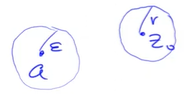
\includegraphics[width=5    cm]{assets/04-functions-of-complex-variables/fractional-linear-functions.png}
            \end{center}

            То же самое верно, если дописать замыкание: $f(|z - a| < r) \cap Cl \; f(0 < |z - z_0| < \varepsilon) = \emptyset$ --  противоречие (т.к. замыкание это все $\mathbb{C}$).
        }
        \item {
            $z_0 \neq \infty$ -- полюс. Тогда из однолистности это полюс первого порядка. А тогда
            $g(z) = f(z) - \frac{c}{z - z_0} \in H(\bar{\mathbb{C}}) \Rightarrow g(z) = const \Rightarrow f(z) = \frac{c}{z - z_0} + const$ 
        }
        \item {
            $z_0 = \infty$ -- полюс, тогда $g(z) = f(z) - cz \in H(\bar{\mathbb{C}}) \Rightarrow g(z) = const \Rightarrow f(z) = cz + const$.
        }
        \item {
            $z_0$ -- устранимая особая точка $\implies f \in H(\bar{\mathbb{C}}) \implies f \equiv const \implies$ нет однолистности $f$ -- противоречие.
        }
    \end{enumerate}
\end{proof}

\begin{consequence}
    Если функция $f \in H(\mathbb{C})$ и однолистная, то $f$ линейная.
\end{consequence}

\begin{proof}
    $z_0 = \infty$ в теореме.
\end{proof}

\Subsection{Производящие функции}

\begin{definition}
    Есть последовательность $a_0, a_1, \ldots$. Производящая функция последовательности
    $\mathcal{A}(z) = \sum_{n = 0}^{\infty} a_nz^n$.

    Мы хотим, чтобы ряд сходился при $|z| < R$ для какого-то $R > 0$
\end{definition}

\begin{example}
    \textbf{Задача о размене}

    Есть монетки $1, 2, 5, 10$ рублей. Интересуемся, каким количеством способов мы можем разменять $n$ рублей, если запас монет не ограничен, пусть это число равно $a_n$.

    Вместо формулы для этих коэффициентов будет искать формулу для ряда:

    $\mathcal{A}(z) := \sum_{n=0}^{\infty} a_n z^n$.

    Это будет равно:

    $\mathcal{A}(z) = (1 + z + z^2 + \ldots)(1 + z^2 + \ldots)(1 + z^5 + z^{10} + \ldots)(1 + z^{10} + z^{20} + \ldots)$ и 
    раскроем все скобки.

    Коэффициент при $z^n = z^a \cdot z^{2b} \cdot z^{5c} \cdot z^{10d}$, где $a + 2b + 5c + 10d = n$.
    Тогда коэффициент $a_n$ -- число решений уравнения $a + 2b + 5c + 10d = n$ в неотрицательных целых числах.

    $\mathcal{A}(z) = \frac{1}{1 - z} \cdot \frac{1}{1 - z^2} \cdot \frac{1}{1 - z^5} \cdot \frac{1}{1 - z^{10}}$.
\end{example}

\begin{definition}
    $H \subset \mathbb{N}, \ p(n, H)$ - количество способов представить $n$ в виде суммы слагаемых из $H$.

    $\mathcal{F}_{H}(z) = \sum_{n=0}^{\infty} p(n, H) z^n = \prod_{k \in H} \frac{1}{1 - z^k}$

    Если каждое слагаемое можно брать $\leqslant m$, то $\prod_{k \in H} \underbrace{\frac{1 - z^{(m+1)k}}{1 - z^k}}_{=(1 + z^k + z^{2k} + \dots + z^{mk})}$
\end{definition}

\begin{definition}
    Число разбиений $n$ на натуральные слагаемые $p(n) = p(n, \mathbb{N})$.
\end{definition}

\begin{theorem}
    $f(z) = \sum_{n = 0}^{\infty} p(n) z^n = \prod_{k=1}^{\infty} \frac{1}{1 - z^k}$ -- сходится при $|z| < 1$
    и $p(n) = \frac{1}{2\pi i} \int_{|z| = r} \frac{f(z)}{z^{n + 1}} \, dz$ при $0 < r < 1$.
\end{theorem}

\begin{proof}
    $\ln \left (\prod_{k=1}^{\infty} \left | \frac{1}{1 - z^k} \right | \right ) = \sum_{k=1}^{\infty} -\ln |1 - z^k| = (*)$ -- покажем, что этот ряд сходится.

    \begin{enumerate}
        \item $\ln{(1 - t)} \geq -t - t^2 \implies -\ln{(1 - t)} \leq t + t^2$
        \item $\ln{|1 - z^k|} \geq \ln{(1 - |z|^k)} \implies -\ln{|1 - z^k|} \leq -\ln{(1 - |z|^k)} \leq |z|^k + |z|^{2k}$
    \end{enumerate}

    Из пункта (2) выше получаем, что $(*) \leq \sum_{k=1}^{\infty} |z|^k + \sum_{k=1}^{\infty} |z|^{2k} < +\infty$ -- справа от нер-ва сумма рядов сх-ся, тогда и $(*)$ тоже.
    
    Проверим, что аргумент ничего не испортит:

    % $\ln (1 + t) \geqslant t - t^2$ при $|t| < 1$. $\ln (1 - |z|^k) \geqslant |z|^k - |z|^{2k}$ и 
    % $0 \leqslant -\ln |1 - z^k| \leqslant |z|^k + |z|^{2k}$.

    $\arg \left ( \frac{1}{1 - z^k} \right ) = -\arg (1 - z^k)$
    
    $|\arg (1 - z^k)| \leqslant \arcsin |z|^k \leqslant 2|z|^k$
    
    Действительно, аргумент ничего не портит.
\end{proof}

\begin{remark}
    \textbf{Теорема Харди-Рамануджана}

    $p(n) \sim \frac{1}{4n\sqrt{3}} e^{\pi \sqrt{\frac{2}{3}}\sqrt{n}}$
\end{remark}

\begin{theorem}
    \textbf{Эйлера}

    Количество разбиений $n$ на нечётные слагаемые равно количеству разбиений
    $n$ на различные слагаемые
\end{theorem}

\begin{proof}
    Для различных слагаемых $\prod_{k = 1}^{\infty} (1+z^k)$

    Для нечётных слагаемых $\prod_{k = 1}^{\infty} (\frac{1}{1 - z^{2k -1}})$.

    Хотим понять, что это одно и то же.$\prod_{k = 1}^{\infty} (\frac{1}{1 - z^{2k -1}}) =
    \frac{\prod_{n = 1}^{\infty} \frac{1}{1-z^n}}{\prod_{k = 1}^{\infty} \frac{1}{1-z^{2k}}} =
    \prod_{n = 1}^{\infty} \frac{1 - z^{2n}}{1 - z^n} = \prod_{n = 1}^{\infty} (1 + z^n)$
\end{proof}

\begin{example}
    $b_1b_2 \ldots b_k b_{k + 1} \ldots b_{2k}$ счастливый билет, если 
    сумма первых $k$ равна сумме последних $k$.

    Пусть $a_n$ - количество $k$-значных чисел с суммой цифр $n$. То есть 
    количество счастливых билетов $a_0^2 + a_1^2 + \ldots + a_{9k}^2$.

    Пусть $\mathcal{A}(z) = \sum_{n = 0}^{\infty} a_nz^n = (1 + z + z^2 + \ldots + z^9)^k$

    $\mathcal{A}(z) \cdot \mathcal{A}(\frac{1}{z})$ - здесь коэффициент перед $z^0$ - это $a_0^2 + a_1^2 + \ldots$.

    $\frac{1}{2\pi i} \int_{|z| = r} \frac{\mathcal{A}(z) \mathcal{A}\frac{1}{z}}{z} \, dz$ - количество счастливых билетов.
\end{example}

\begin{example}
    \textbf{Диагонализация степенных рядов}

    Пусть дана $f(w, z) = \sum_{n, k = 0}^{\infty} a_{nk} w^n z^k$, а мы хотим найти $g(w) = \sum_{n = 0}^{\infty} a_{nn} w^n$.
    
    Запишем $f(\frac{w}{z}, z) = \sum_{n, k = 0}^{\infty} a_{nk} \frac{w^n}{z^n} z^k$, видно, что нас интересует коэффициент перед $z_0$ (если мы его найдет, то получем ответ).


    То есть $g(w) = \frac{1}{2\pi i} \int_{|z| = r} \frac{f(\frac{w}{z}, z)}{z} \, dz = \frac{1}{2\pi i} \int_{|z| = r} \sum_{n, k = 0}^{\infty} a_{nk} w^n z^{k - n - 1} \, dz =$
    
    $= \frac{1}{2\pi i} \sum_{n, k = 0}^{\infty} w^n a_{nk} \underbrace{\int_{|z| = r} z^{k - n - 1} \, dz}_{=0, \text{ при } k \not = n, \ 2\pi i \text{ иначе}} = \frac{1}{2\pi i} \sum_{n = 0}^{\infty} w^n a_{nn} 2\pi i = g(w)$


    Чтобы можно было переставить интеграл и сумму, нужна равномерная сходимость. То есть нужно попасть строго внутрь круга сходимости ряда $\sum |a_{nk}| r^{k-1} \left |\frac{w}{z} \right |^n$.
    
    Пусть радиус сх-ти для $z$ и для $w$ равен $R$, тогда нужно, чтобы $r < R, \left|\frac{w}{r}\right| < R$.

    % Нужно $\left | \frac{w}{z} \right | < \rho$. Берём
    % радиус сходимости для $z$, для $w$, всё половиним, ещё на что-то умножаем.

    \bigskip

    Давайте теперь воспользуемся полученной схемой на конкретном примере:
    
    пусть $f(w, z) = \sum_{n, k = 0}^{\infty} \binom{n+k}{k}w^nz^k = \sum_{m = 0}^{\infty} \sum_{k = 0}^{m} \binom{m}{k} w^{m - k}z^k = \sum_{m = 0}^{\infty} (w + z)^m = \frac{1}{1 - w - z}$.


    Найдем $\frac{1}{2\pi i} \int_{|z| = r} \frac{f(\frac{w}{z}, z)}{z} \, dz = \frac{1}{2\pi i} \int_{|z| = r} \frac{dz}{z \left(1 - \frac{w}{z} - z\right)} = -\frac{1}{2\pi i} \int_{|z| = r} \frac{dz}{z^2 - z + w} = (*)$.

    Ищем нули знаменателя, получаем особые точки: $\frac{1 \pm \sqrt{1 - 4w}}{2}$.
    
    В контур попадает только $\frac{1 - \sqrt{1 - 4w}}{2}$, так как второй корень близок к $1$, а этот как раз к нулю.

    $(*) = - \res = -\frac{1}{2z - 1} \bigg |_{z = \frac{1 - \sqrt{1 - 4w}}{2}} = \frac{1}{\sqrt{1 - 4w}}$.

    Мы получили, что $\sum_{n=0}^{\infty} \binom{2n}{n} w^n = \frac{1}{\sqrt{1 - 4 w}}$.

\end{example}

\begin{definition}
    \textbf{Произведение Адамара}

    $\mathcal{A}(z) = \sum_{n = 0}^{\infty} a_nz^n$
    
    $\mathcal{B}(z) = \sum_{n=0}^{\infty} b_nz^n$
    
    $\mathcal{A} \circ \mathcal{B} (z) = \sum_{n = 0}^{\infty} a_nb_n z^n$ 
\end{definition}

\begin{example}
    Как находить произведение Адамара.

    $f(w, z) = \mathcal{A}(z) \mathcal{B}(w) = \sum_{n, k = 0}^{\infty} a_nb_kz^nw^k$.
    
    Нас интересует диагональ этой штуки.
\end{example}

\begin{theorem}
    Произведение Адамара рациональных функций -- рациональная функция
\end{theorem}

\begin{definition}
    Последовательность $\{a_n\}$ -- \textbf{квазимногочлен}, если
    
    $a_n = p_1(n)q_1^n + p_2(n)q_2^n + \ldots + p_k(n)q_k^n$,
    
    где $q_1, \ldots, q_k \in \mathbb{C}$, а $p_1, \ldots, p_k$ -- многочлены с комплексными коэффициентами.
\end{definition}

\begin{lemma}
    $\mathcal{A}(z) = \sum_{n=0}^{\infty} a_n z^n$ -- рациональная фукнция $\Leftrightarrow$ при больших $n \,: \, a_n$ -- квазимногочлен.
\end{lemma}

\begin{proof}
    \begin{enumerate}
        \item {
            $\Rightarrow$. Разложим рациональную функцию на простейшие, $\frac{1}{(1 - qz)^m}$ -- то есть на линейную комбинацию таких.

            $\frac{1}{(1 - z)^m} = \sum_{n = 0}^{\infty} \binom{n + m - 1}{m - 1} z^n$

            Тогда $\frac{1}{(1 - qz)^m} = \sum_{n = 0}^{\infty} \frac{(n + m - 1) \ldots (n + 1)}{(m - 1)!}q^nz^n$
        }
        \item {
            $\Leftarrow$. Достаточно понять, что $a_n = p(n) \cdot q^n$ имеет рациональную производящую функцию, а потом просто сложить в сумму.
            
            Индукция по степени многочлена: 
            
            \begin{enumerate}
                \item {
                    База: $\deg = 0$, $a_n = q^n$ производящая функция $\frac{1}{1 - qz}$.
                }
                \item {
                    Переход: $d - 1 \rightarrow d$.
                    
                    Возьмём конкретный многочлен степени $d$: $\tilde{p}(n) = \frac{(n + d)(n + d - 1) \ldots (n + 1)}{d!}$.

                    Для $b_n = \tilde{p}(n)q^n$ производящая функция $\frac{1}{(1 - qz)^{d + 1}}$.

                    Из $p(n)$ вычтем $c \cdot \tilde{p}(n)$ так, чтобы степень уменьшилась, тогда по предположению индукции -- все работает.
                }
            \end{enumerate}
        }
    \end{enumerate}
\end{proof}

\begin{example}
    \textbf{Метод Дарбу}

    $f(z) = \sum_{n = 0}^{\infty} a_n z^n$ сходится в круге $|z| < R$.
    
    Тогда при любом $r$, таком что $r < R$, ряд $\sum_{n = 0}^{\infty} a_n r^n$ -- сходится и $a_n r^n \rightarrow 0 \Rightarrow a_n = o(r^{-n})$.
    
    Пусть $R$ -- радиус сходимости $f(z) = \sum_{n = 0}^{\infty} a_n z^n$, тогда мы знаем, что на границе круга сходимости есть особая точка.

    Если особых точек конечное число и это полюсы (для простоты будем считать, что одна), то тогда возьмём эту точку и напишем главную часть ряда Лорана:

    $h(z) = \text{главная часть ряда Лорана для функции $f$ в точке $a$}$.
    
    Тогда $g(z) = f(z) - h(z)$ имеет устранимую особую точку $a$. Давайте устраним ее, тогда $g(z)$ голоморфна в точке $a$. Тогда скорее всего её радиус сходимости $\tilde{R} > R$.

    $g(z) = \sum_{n = 0}^{\infty} b_n z^n \Rightarrow b_n =  o((\tilde{R} - \varepsilon)^{-n})$
    
    $h(z) = \frac{c_1}{z - a} + \frac{c_2}{(z - a)^2} + \ldots + \frac{c_r}{(z - a)^r}$, где $r$ -- порядок полюса, у $h(z)$ можно явно выписать коэффициенты (самый быстрорастущий это последний).

    $\frac{1}{(z - a)^r} = \frac{1}{a^r \left(\frac{z}{a} - 1\right)^r} = \frac{(-1)^r}{a^r} \cdot \sum_{n = 0}^{\infty} \binom{n + r - 1}{r - 1} \left( \frac{z}{a} \right)^n$.

    Оценим биномиальный коэффициент: $\binom{n + r - 1}{r - 1} = \frac{(n + r - 1) \ldots (n + 1)}{(r - 1)!} \sim \frac{n^{r - 1}}{(r - 1)!}$.
    
    Тогда $a_n \sim c_r \cdot \frac{n^{r - 1}}{(r - 1)!} \cdot \frac{(-1)^r}{a^{n + r}}$.
\end{example}

\begin{theorem}
    Пусть $f \in H(|z| < R)$, где $R > 1$ и $f(1) \neq 0$.
    
    Пусть $\frac{f(z)}{(1 - z)^\alpha} = \sum_{n = 0}^{\infty} b_n z^n, \ \alpha \in \mathbb{R}, \ \alpha \neq 0, -1, -2 \ldots$

    Тогда $b_n \sim f(1) \cdot \binom{n + \alpha - 1}{n} \sim f(1) \cdot \frac{n^{\alpha - 1}}{\Gamma (\alpha)}$
\end{theorem}

\begin{proof}

    Возьмём $1 < r < R$ и разложим $f(z) = \sum_{n = 0}^{\infty} a_n z^n$.
    
    Ряд сходится в точке $z = r \Rightarrow a_n = o(r^{-n})$.

    $\frac{1}{(1 - z)^\alpha} = \sum_{n = 0}^{\infty} \underbrace{\binom{n + \alpha - 1}{n}}_{=\frac{(n + \alpha - 1)(n + \alpha - 2) \ldots \alpha}{n!}} z^n$.

    Получаем:
    
    $\frac{f(z)}{(1 - z)^\alpha} = \sum a_n z^n \cdot \sum \binom{n + \alpha - 1}{n} z^n$
    
    $b_n = a_n \binom{\alpha - 1}{0} + a_{n - 1}\binom{\alpha}{1} + \ldots + a_0 \binom{n + \alpha - 1}{n} = \binom{n + \alpha - 1}{n} (a_0 + \frac{n}{n + \alpha - 1} a_1 + \frac{n(n - 1)}{(n + \alpha - 1)(n + \alpha - 2)} a_2 + \ldots + (\ldots) \cdot a_n)$, где все коэффициенты при $a_i$ стремятся к $1$.

    Хотим сказать, что $b_n \sim \binom{n + \alpha - 1}{n} \cdot (a_0 + a_1 + \ldots + a_n) \sim \binom{n + \alpha - 1}{n} \cdot f(1) =$
    
    $= \frac{\alpha(\alpha - 1) \ldots (\alpha + n - 1)}{n!} f(1) \rightarrow \frac{n^{\alpha - 1}}{\Gamma(\alpha)} \cdot f(1)$ -- последний переход из формулы Эйлера-Гаусса.

    Осталось понять, что $\Delta_n = (a_0 + \frac{n}{n + \alpha - 1}a_1 + \frac{n(n - 1)}{(n + \alpha - 1)(n + \alpha -2)}a_2 + \ldots + (\ldots)\cdot a_n) - (a_0 + a_1 + \ldots +a_n) \rightarrow 0$.
    
    Мы знаем, что $a_n = \mathcal{O}(r^{-n}) \Rightarrow |a_n| \leqslant \frac{C}{r^n}$. 
    
    Тогда $|\Delta_n| \leqslant
    \underbrace{|a_1| \left|\frac{n}{n + \alpha - 1} - 1\right| +
    |a_2| \left|\frac{n (n - 1)}{(n + \alpha - 1) (n + \alpha - 2)} - 1\right| +
    \ldots +
    |a_m| \left|(\ldots) - 1\right|}_{\text{конечное число слагаемых } \rightarrow 0} +$
    
    $+ \left(\frac{C}{r^{m + 1}} + \frac{C}{r^{m + 2}} + \ldots\right)$
    
    Подберём так $m$ чтобы $\sum \frac{C}{r^{m + i}} \leqslant \varepsilon$. И тогда всё выполнилось при больших $n$.
\end{proof}

\begin{example}
    \begin{enumerate}
        \item {
            $f(z) = \frac{\sqrt{2 - z}}{(1 - z)^2}$
            
            Здесь круг сходимости $|z| < 1$, особая точка $z = 1$ -- полюс второго порядка.
            
            Главная часть ряда Лорана: $\frac{a}{1 - z} + \frac{b}{(1 - z)^2} = -\frac{1}{2} \cdot \frac{1}{1 - z} + \frac{1}{(1 - z)^2}$.
            
            Здесь $b = \sqrt{2 - 1} = 1$, $a = \res_{z = 1} = ((1 - z)^2 f(z))' \bigg|_{z = 1} = (\sqrt{2 - z})' \bigg|_{z = 1} = \frac{-1}{2 \sqrt{2 - z}} \bigg|_{z = 1} = -\frac{1}{2}$.

            $g(z) = f(z) - \frac{1}{(1 - z)^2} + \frac{1}{2} \cdot \frac{1}{1 - z}$  -- голоморфна в $z = 1$, тогда $g \in H(|z| < 2)$.

            Пусть $f(z) = \sum_{n=0}^{\infty} a_n z^n, \ g(z) = \sum_{n=0}^{\infty} b_n z^n, \ b_n = o\left( \frac{1}{(2 - \varepsilon)^n} \right)$

            $a_n = b_n -\frac{1}{2} + n + 1 = n + \frac{1}{2} + o \left( \frac{1}{(2 - \varepsilon)^n} \right)$
        }
        \item {
            $f(z) = \frac{e^z}{\sqrt{1 - z}} = \sum_{n = 0}^{\infty} a_n z^n$, круг сходимости $|z| < 1$, но $z = 1$ не полюс, а точка ветвления.

            $g(z) = \frac{e^z}{\sqrt{1 - z}} - \frac{e}{\sqrt{1 - z}} = \frac{e}{\sqrt{1 - z}} (e^{z - 1} - 1) = \frac{e}{\sqrt{1 - z}} (1 - z) \underbrace{\frac{e^{z - 1} - 1}{1 - z}}_{=h(z) \text{, голоморфна в 1}} = e\sqrt{1 - z} h(z)$, где на самом деле $h(z) = \frac{1 + (z - 1) + \frac{(z - 1)^2}{2} + \ldots}{1 - z} \in H(\mathbb{C})$.

            $g(z) = \sum b_n z^n$, из теоремы имеем $b_n \sim h(1) \frac{n^{-\frac{3}{2}}}{\Gamma (\frac{1}{2})} = -\frac{1}{\sqrt{\pi} n \sqrt{n}}$

            $e \sqrt{1 - z} = e \sum_{n=0}^{\infty} c_n z^n$.
            
            Тогда $a_n = e \cdot c_n + b_n = \frac{e \cdot \binom{2n}{n}}{4^n} + b_n = e \cdot \underbrace{\frac{\binom{2n}{n}}{4^n}}_{\sim \frac{1}{\sqrt{\pi n}}} + \mathcal{O}\left(\frac{1}{\sqrt{n^3}}\right)$.
            
            $\sqrt{1 - 4z} = \sum_{n=0}^{\infty} \binom{2n}{n} z^n$ -- с одной из прошлый лекций. Тогда $\sqrt{1 - z} = \sum \binom{2n}{n} \frac{z^n}{4^n}$.
            
            И тогда $a_n = e \cdot \frac{\binom{2n}{n}}{4^n} + b_n = e \cdot \frac{\binom{2n}{n}}{4^n} + \mathcal{O}\left(\frac{1}{n^{\frac{3}{2}}}\right)$
        }
    \end{enumerate}
\end{example}

\begin{example}
    \textbf{Метод Лапласа}

    Есть $2k$-значный номер, интересуемся количеством таких номеров, что сумма первых $k$ знаков равна сумме последних $k$ (счастливые билеты).

    Пусть $a_k = $ количество $2k$ значных счастливых билетов.

    $a_k = \frac{1}{2\pi i} \int_{|z| = 1} \mathcal{A}(z) \mathcal{A}(\frac{1}{z}) \frac{dz}{z}$
    
    $\mathcal{A}(z) = (1 + z + z^2 + \ldots + z^9)^k = \left( \frac{1 - z^{10}}{1 - z} \right)^k$

    Тогда $a_k =
    \frac{1}{2 \pi i} \int_{|z| = 1} \left( \frac{(1 - z^{10})(1 - z^{-10})}{(1 - z)(1 - \frac{1}{z})} \right)^k \frac{dz}{z} =
    \frac{1}{2\pi i} \int_{|z| = 1} \left( \frac{2 - z^{10} - z^{-10}}{2 - z - \frac{1}{z}} \right)^k \frac{dz}{z} = (*)$

    Делаем замену: $z = e^{it}, \ dz = i \cdot e^{it} dt$.
    
    $(*) = \frac{1}{2\pi i} \int_{0}^{2\pi} \left( \frac{2 - e^{10 it} - e^{-10 it}}{2 - e^{it} - e^{-it}} \right)^k \frac{i e^{it}}{e^{it}} \, dt = $
    
    $= \frac{1}{2\pi} \int_{0}^{2\pi} \left( \frac{2 - 2 \cos{(10 t)}}{2 - 2\cos{t}} \right)^k \, dt = \frac{1}{2\pi} \int_{0}^{2\pi} \left( \frac{2\sin^2{(5 t)}}{2 \sin^2{\frac{t}{2}}} \right)^k \, dt =$
    
    Делаем доп. замену: $s = \frac{t}{2}, \ 1 - \cos{t} = 2 sin^2{\frac{t}{2}}$.

    $= \frac{1}{2\pi} \int_{0}^\pi 2\left( \frac{\sin {(10s)}}{\sin s} \right)^{2k} \, ds \underbrace{=}_{\text{т.е. симметрия отн. } \frac{\pi}{2}} \frac{2}{\pi} \int_{0}^{\frac{\pi}{2}} \left( \frac{\sin (10x)}{\sin x} \right)^{2k} ds$.


    Можно выловить скорость роста интеграла: поведение определено точкой максимума у $\frac{\sin{(10x)}}{\sin{x}}$.

    \begin{center}
        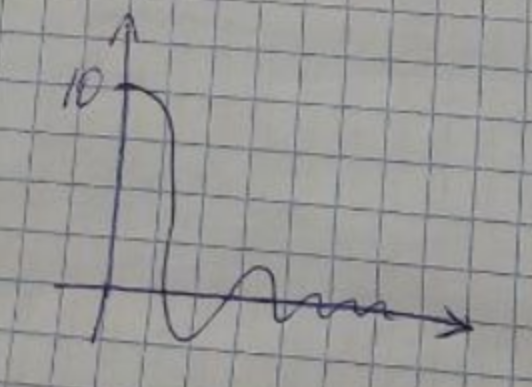
\includegraphics[width=6cm]{assets/04-functions-of-complex-variables/laplasian-method.png}
    \end{center}

    \begin{enumerate}
        \item В нуле максимум равен $10$
        \item В окрестности нуля разложим по Тейлору
        \item Остальное просто оценим
    \end{enumerate}

    $\int_{0}^{\frac{\pi}{2}} \left( \frac{\sin{(10x)}}{\sin{x}} \right)^k dx = \int_{0}^{\varepsilon} + \int_{\varepsilon}^{\frac{\pi}{2}}$


    \begin{enumerate}
        \item {
            Посмотрим на окрестность нуля.

            Раскладываем по Тейлору:

            $\frac{\sin{(10x)}}{\sin{x}} = \frac{10x - \frac{(10x)^3}{6} + \mathcal{O}(x^5)}{x - \frac{x^3}{3} + \mathcal{O}(x^3)} = 10 \cdot \frac{1 - \frac{100 x^2}{6} + \mathcal{O}(x^4)}{1 - \frac{x^2}{6} + \mathcal{O}(x^4)} =$
            
            $= 10 (1 - \frac{100}{6} x^2 + \mathcal{O}(x^4)) (1 + \frac{x^2}{6} + \mathcal{O}(x^4)) = 10 (1 - \frac{33}{2} x^2 + O(x^4))$

            Под интегралами у нас это степенная функция, поэтому распишем логарифм от нашего выражения:

            $\ln \frac{\sin(10x)}{\sin{x}} = \ln \left(10 (1 - \frac{33}{2} x^2 + O(x^4))\right)$

            $\left( \frac{\sin(10x)}{\sin{x}} \right)^{2k} = e^{2k \ln\left( 10 (1 - \frac{33}{2} x^2 + O(x^4)) \right)} = 10^{2k} \cdot e^{-33 k x^2} \cdot e^{\mathcal{O}(2k x^4)}$

            Подставим это в интеграл с $\varepsilon$:

            $k \varepsilon^4 \rightarrow 0$,

            $\int_{0}^{\varepsilon} 10^{2k} e^{-33k x^2} \underbrace{e^{\mathcal{O}(k x^4)}}_{= e^{\mathcal{O}(k \varepsilon^4)}, \text{ выберем $\varepsilon$ так, что } = 1 + \mathcal{O}(k \varepsilon^4)} = 10^{2k} \left( 1 + \mathcal{O}(k \varepsilon^4) \right) \int_{0}^{\varepsilon} e^{-33 k x^2} dx = (')$

            Делаем замену: $y = \sqrt{33k} x$.

            $(') = 10^{2k} \left(1 + \mathcal{O}(k \varepsilon^4)\right) \int_{0}^{\varepsilon \sqrt{33k}} e^{-y^2} \frac{1}{\sqrt{33k}} dy \sim 10^{2k} \frac{1}{\sqrt{33k}} \cdot \frac{\sqrt{\pi}}{2} = ('')$

            Хотим, чтобы $\varepsilon \sqrt{33} \rightarrow +\infty$, тогда $('') \rightarrow \int_{0}^{+\infty} = \frac{\sqrt{\pi}}{2}$.
            
            Для этого подойдет $\varepsilon = \sqrt{1}{k^{\frac{1}{3}}}$.
        }
        \item {
            Посмотрим на остальное.

            $\int_{\frac{\pi}{10}}^{\frac{\pi}{2}} \left( \frac{\sin{(10x)}}{\sin{x}} \right)^{2k} dx \leq \underbrace{\frac{\pi}{2}}_{\text{длина отрезка $\leq$ этого}} \left( \frac{1}{\sin{(\frac{\pi}{10})}} \right)^{2k}$

            если $\frac{\pi}{10}$ не подойдет, то немного подвинуть.

            Смотрим на вторую часть:

            $\int_{\varepsilon}^{\frac{\pi}{10}} \left( \frac{\sin{(10x)}}{\sin{x}} \right)^{2k} \underbrace{\leq}_{\text{т.к. функция убывает}} \frac{\pi}{10} \left(\frac{\sin{(10 \varepsilon)}}{\sin{\varepsilon}}\right)^{2k} \underbrace{=}_{\text{считали в предыдущем пункте}} \frac{\pi}{10} 10^{2k} \underbrace{e^{-33k \varepsilon^2}}_{\text{быстро убывает}} \underbrace{e^{\mathcal{O}(k \varepsilon^4)}}_{\sim 1}$
        }
    \end{enumerate}


    Метод работает в случае $\int_{a}^{b} \left(f(x)\right)^n$ и $n \rightarrow \infty$.
\end{example}
\Section{Ряды Фурье}{Дмитрий Артюхов}
\Subsection{Пространства Лебега}

\begin{definition}
    $\mu$ -- мера, $p \geq 1$.

    $L^{p} (E, \mu) := \{f : E \rightarrow \bar{\mathbb{R}}$ - измеримые, т.ч. $\int_{E} |f|^p d\mu < \infty\}$  -- векторное пр-во.

    $|| f ||_p = \left( \int_{E} |f|^p d\mu \right)^{\frac{1}{p}}$

    \begin{enumerate}
        \item Нер-во треугольника -- нер-во Минковского: $||f+g||_p \leq ||f||_p + ||g||_p$.
        \item Неотрицательность: $|| f ||_{p} \geq 0$.
        \item Константа выносится: $|| \alpha \cdot f ||_p = |\alpha| \cdot ||f||_p$.
        \item Но в нуле не всегда значение равно нулю: $||f||_p = 0 \Rightarrow$ интеграл от неотрицательной функции $|f|^p$ равен нулю $\Rightarrow$ $f = 0$ \textbf{почти везде}.
    \end{enumerate}

    Рассматриваем не функции, а классы эквивалентности с точностью до совпадения почти везде.

    Проблема: нет значения функции в точке.
\end{definition}

\begin{definition}
    \textbf{Существенный супремум} ($esssup$ или $rraisup$)

    $a$ -- существенный супремум функции $f: E \rightarrow \bar{\mathbb{R}}$,

    если $a = \inf \{ c \in \mathbb{R} : f(x) \leq c \text{ при почти всех $x \in E$}\}$.
\end{definition}

\begin{properties}
    \begin{enumerate}
        \item $esssup f \leq \sup f$
        \item {
            $f(x) \leq esssup f$ при почти всех $x$

            \begin{proof}
                $a := esssup f \implies \exists e_n : \ \mu e_n = 0$ (т.е. существует мн-во $e_n$ нулевой меры), т.ч. $f(x) \leq a + \frac{1}{n}$, $\forall x \in E \setminus e_n$

                $e = \bigcup_{n=1}^{\infty} e_n, \ \mu e = 0$ и $f(x) = a + \frac{1}{n}, \ \forall x \in E \setminus e \implies f(x) \leq a \ \forall x \in E \setminus e$.
            \end{proof}
        }
    \end{enumerate}
\end{properties}

\begin{definition}
    $L^{\infty} (E, \mu) := \{ f: E \rightarrow \bar{\mathbb{R}}$ - измеримые, т.ч. $esssup_{x\in E} |f(x)| < +\infty \}$ - векторное пр-во.

    Заведем норму для данного векторного пр-ва: $|| f ||_{\infty} := esssup_{x\in E} |f(x)|$.

    \begin{enumerate}
        \item Константа выносится
        \item Нер-во треугольника есть
        \item Функция 0 почти везде, но все же не везде
    \end{enumerate}

    % Тут лекция, видимо, закончилась
    Рассмотрим классы эквивалентности...

    \textbf{Важный частный случай ($X = \mathbb{N}$)}

    $X = \mathbb{N}$, $\mu$- считающая мера, тогда:

    1. $l^p = \{ (x_1, x_2, \ldots) \text{ - последовательность} \, : \, \sum_{k = 1}^{\infty} |x_k|^p < +\infty \}$

        Норма в данном случае: $|| x ||_p = \left( \sum_{k = 1}^{\infty} |x_k|^p \right)^{\frac{1}{p}}$

    2. $l^\infty = \{ (x_1, x_2, \ldots) \, : \, \sup |x_k| < +\infty \}$

        Норма в данном случае: $|| x ||_{\infty} = \sup_{k \in \mathbb{N}} |x_k|$
\end{definition}

\begin{theorem}
    \textbf{Вложение пространств Лебега}

    Пусть $\mu E < +\infty$ и $1 \leqslant p \leqslant q \leqslant +\infty$.

    Тогда $L^q (E, \mu) \subset L^p (E, \mu)$ и $||f||_p \leqslant ||f||_q \cdot (\mu E)^{\frac{1}{p}-\frac{1}{q}}$
\end{theorem}

\begin{proof}
    Пусть $q < +\infty$.

    Напишем неравенство Гёльдера:

    $\int_E |f|^p \cdot 1 \, d\mu \leqslant \left( \int_E \left(|f|^p\right)^{r} \, d\mu \right)^{\frac{1}{r}} \left( \int 1^{r'} \, d\mu \right)^{\frac{1}{r'}} = (*)$

    Здесь $\frac{1}{r} + \frac{1}{r'} = 1, \ r = \frac{q}{p} \Rightarrow \frac{1}{r'} = \frac{q - p}{q}$.

    Тогда $(*) = \left(||f||_q\right)^p \cdot (\mu E)^{\frac{q - p}{q}} \Rightarrow_{\text{извлекаем корень $p$-ой степени слева и справа}} ||f||_p \leqslant ||f||_q (\mu E)^{\frac{q - p}{pq}}$

    Пусть $q = +\infty$, тогда $||f||_p^p = \int_E |f|^p \, d\mu \leqslant \int_E ||f||_\infty^p \, d\mu = \mu E ||f||_\infty^p$

    \begin{remark}
        Для $\mu E = +\infty$ вложений нет
    \end{remark}
\end{proof}

\begin{theorem}
    $L^p (E, \mu)$ - полное, где $1 \leqslant p \leqslant +\infty$
\end{theorem}

\begin{proof}
    Только для $p < +\infty$

    \underline{Идейно, что хотим доказать}: пространство является полным, если $\forall$ фундаментальная последовательность сходится, и её предел принадлежит данному пространству.

    Пусть $f_n$ - фундаментальная последовательность функций. Мы знаем по определению фундаментальности:

    $\forall \, \varepsilon > 0 \, \exists N \, : \, \forall \, m, n \geqslant N \, : \, ||f_n - f_m||_p < \varepsilon$

    Выберем некоторую подпоследовательность $f_{n_k}$:

    1. Берём $\varepsilon_1 = \frac{1}{2}$, по нему возьмем $N_1$ из определения, далее определим $n_1 := N_1$.

    2. Далее возьмем $\varepsilon_2 = \frac{1}{2^2}$, по нему возьмем $N_2$ из определения, далее определим $n_2 := max(N_2, \ n_1 + 1)$.

    И так далее.\newline

    Получилось, что $n_1 < n_2 < n_3 < \ldots$, а также $||f_{n_k} - f_n|| < \frac{1}{2^k}$ при $n \geqslant n_k$, в частности
    $||f_{n_k} - f_{n_{k + 1}}|| < \frac{1}{2^k}$ - так строили подпоследовательность.

    Рассматрим $\Sigma_{k=1}^{+\infty} || f_{n_k} - f_{n_{k+1}} ||_p$:

    $$ \Sigma_{k=1}^{+\infty} || f_{n_k} - f_{n_{k+1}} ||_p < \Sigma_{k=1}^{+\infty} \frac{1}{2^k} = 1$$

    Тогда $\sum_{k = 1}^\infty ||f_{n_{k}} - f_{n_{k + 1}}||_p < 1$.

    Пусть $S(t) = \sum_{k = 1}^\infty |f_{n_{k}}(t) - f_{n_{k + 1}}(t)|$. $S \, : \, E \to \overline{\mathbb{R}}$.

    Пусть $S_m(t) := \sum_{k = 1}^m |f_{n_{k}}(t) - f_{n_{k + 1}}(t)|$ - частичная сумма.

    $||S_n||_p \leqslant ||f_{n_1} - f_{n_2}||_p + ||f_{n_2} - f_{n_3}||_p + \ldots + ||f_{n_m} - f_{n_{m + 1}}||_p < 1$ - норма суммы меньше суммы норм.

    Следовательно: $||S_n||_p < 1 \quad (*)$.\newline

    Теперь рассмотрим $|| S ||^p_p$:

    \underline{Напоминание (Лемма Фату)}: Если $f_n \geq 0$, то $\int_E{\underline{\lim}{f_n d \mu}} \leq \underline{\lim}{\int_E{f_n d \mu}}$.

    $||S||^p_p = \int_{E} |S(t)|^p \, dt = \int_E \lim_{n \to +\infty} |S_m(t)|^p \, dt \underbrace{\leqslant}_{\text{л. Фату}} \underline{\lim} \int_E |S_m(t)|^p \, dt =
    \underline{\lim} ||S_m ||^p_p \underbrace{\leqslant}_{\text{т.к. верно (*)}} 1 $.

    Так как по определению $S = \lim_{n\rightarrow +\infty} S_n$ (т.е. предел $S_n$ существует и равен $S$), то $\underline{\lim} = \lim = \bar{\lim}$.

    $ \implies \int_E |S(t)|^p \, dt < +\infty \implies S(t) < +\infty$ при почти всех $t \in E$.

    Тогда $S(t) = \Sigma_{k=1}^{+\infty} |f_{n_k}(x) - f_{n_{k+1}}(x)| < +\infty$ -- ряд из суммы неотрицательных слагаемых ограничен, значит он сходится. Если мы рассматривем данный ряд без модулей, то такой ряд уже имеет абсолютную сходимость почти везде, а значит и обычную почти везде тоже.\newline

    Заметим, что: $f_{n_1} + \Sigma_{k=1}^{m} (f_{n_{k+1}} - f_{n_k}) = \Sigma_{k=2}^{m+1} f_{n_k} - \Sigma_{k=2}^{m} f_{n_k} = f_{n_{m+1}}$ -- так как сумма ряда сходится почти везде, то $f_{n_m}$ сходятся при почти всех $t \in E \Rightarrow \lim_{m\rightarrow +\infty} f_{n_m} = f$.\newline

    Сейчас мы показали обычную сходимость, нужно показать сходимость по норме пр-ва, т.е. $|| f_n - f ||_p \rightarrow 0$:

    Возьмём $n \geqslant n_k$, тогда:

    $$||f_n - f|| \leqslant \underbrace{||f_n - f_{n_k}||}_{\cdot < \frac{1}{2^k}} + \underbrace{||f_{n_k} - f||}_{\cdot < \frac{1}{2^k} \ (**)} \leqslant \frac{1}{2^{k-1}} \rightarrow 0$$

    Нужно показать, что (**) верно:

    Мы уже знаем, что $\lim_{k\rightarrow +\infty} f_{n_k} = f$ -- почти везде, тогда рассмотрим $|| f_{n_k} - f ||^p_p$:

    $$|| f_{n_k} - f ||^p_p = \lim_{k\rightarrow \infty} \int_{E} |f_{n_k} - f|^p \,d\mu \underbrace{=}_{(***)} \int_{E} \underbrace{\lim_{k\rightarrow \infty} |f_{n_k}-f|^p}_{\text{Почти везде $= 0$}}\, d\mu$$

    Выше мы использовали теорему Лебега о предельном переходе (о мажорируемой сходимости), для того, чтобы ее использовать в (***) нужно показать, что $|f_{n_k} - f|^p \leq F$, где $F$ -- некоторая суммируемая функция (т.е. искомая суммир. мажоратна):

    Ранее мы уже показали, что $f_{n_{m+1}} = f_{n_1} + \Sigma_{k=1}^{m} (f_{n_{k+1}} - f_{n_k})$ -- заметим, что если написать $f_{n_k} + \Sigma_{i=k}^{m} (f_{n_{i+1}} - f_{n_i}) = f_{n_{m+1}}$, то сумма не изменится. Тогда рассмотрим произвольное $k$ и устремим $m \rightarrow +\infty$:

    $$ f(t) = f_{n_k} + \Sigma_{i=k}^{+\infty} (f_{n_{i+1}} - f_{n_i}) \Rightarrow $$
    $$ \Rightarrow |f(t) - f_{n_k}(t)| = \left|\Sigma_{i=k}^{+\infty} (f_{n_{i+1}} - f_{n_i})\right| \leq \Sigma_{i=k}^{+\infty} |f_{n_{i+1}} - f_{n_i}| \leq S(t) \underbrace{<}_{\text{т.к. ранее показали}} +\infty \Rightarrow$$
    $$ \Rightarrow \forall k: |f - f_{n_k}| \leq S^p(t) < +\infty $$

    Получаем суммируемую мажоратну $S^p(t) \Rightarrow$ переход (***) корректен. А значит и утверждение (**) тоже корректно, следовательно у нашей фундаментальной последовательности $f_n$ есть сходимость по норме. \newline

    Осталось показать, что предел $f = \lim_{k\rightarrow +\infty} f_n$ принадлежит пространству $\Leftrightarrow$ его норма конечна (см. опр. $L^p (E, \mu)$):

    Применим нер-во Минковского для $f = f_{n_k} + \Sigma_{i=k}^{+\infty} (f_{n_{i+1}} - f_{n_i})$:

    $$ \left(\int_{E} |f|^p \, d\mu\right)^{\frac{1}{p}} \leq \underbrace{\left(\int_{E} |f_{n_k}|^p \, d\mu\right)^{\frac{1}{p}}}_{\cdot < +\infty \text{ т.к. $f_{n_k} \in L^p(E, \mu)$}} + \underbrace{\left(\int_{E} |\Sigma|^p \, d\mu\right)^{\frac{1}{p}}}_{\cdot \leq \left(\int_{E} |S(t)|^p \, d\mu\right)^{\frac{1}{p}} < +\infty} < +\infty \Rightarrow$$
    $$ \Rightarrow \text{т.к. $p < +\infty$: } \int_{E} |f|^p \, d\mu < +\infty $$

    Следовательно, $f \in L^p(E, \mu)$, чтд.
\end{proof}

\begin{definition}
    $(X, \rho)$ - метрическое пространство и $A \subset X$. $A$ \textbf{всюду плотно} в $X$ (или \textbf{плотно} в $X$), если $Cl A = X$.

    \begin{example}
        $X = \mathbb{R}$ и $A = \mathbb{Q}$.
    \end{example}
\end{definition}

\begin{definition}
    $f \, : \, E \to \mathbb{R}$ называется ступенчатой, если она измерима и у неё конечное число значений.
\end{definition}

\begin{lemma}
    $1 \leqslant p < +\infty, \varphi$ ступенчатая $\in L^p (E, \mu)$

    Тогда $\mu E \{ \varphi \neq 0 \} < +\infty$
\end{lemma}

\begin{proof}
    $|\varphi|$ - рассмотрим положительные значения, их конечное число, значит среди них есть наименьшее. Тогда
    на множестве $E \{ \varphi \neq 0 \}, |\varphi| \geqslant m$

    Тогда $\int_E |\varphi|^p \, d\mu = \int_{E \{ \varphi \neq 0 \}} |\varphi|^p \, d\mu \geqslant \int_{E \{ \varphi \neq 0 \}} m^p \, d\mu = m^p \mu E \{ \varphi \neq 0 \}$
\end{proof}

\begin{theorem}
    $1 \leqslant p \leqslant +\infty$

    Тогда множество ступенчатых функций из $L^p (E, \mu)$ плотно в $L^p (E, \mu)$.
\end{theorem}

\begin{proof}

    Идейно данная теорема утверждает, что любая функция из $L^p (E, \mu)$ сколь угодно хорошо может быть приближена ступенчатыми функциями.

    \begin{enumerate}
        \item {
            $p = +\infty$. Идейно: хотим д-ть, что замыкание мн-ва ступенчатых ф-й является всем мн-вом $L^p (E, \mu)$ (\textbf{def:} замыкание -- это мн-во предельных точек), т.е. нужно показать, что любая точка мн-ва $L^p (E, \mu)$ является предельной для мн-ва ступенчатых функций $\Rightarrow$ любая функция $f \in L^p (E, \mu)$ сколь угодно хорошо приближается ступенчатыми функциями.


            Возьмём $f \in L^\infty (E, \mu), f \geqslant 0$. Выберем такую $f$, что она ограничена (всегда можем так сделать, так как мы рассматривем класс эквивалентности, значит нужно выбрать ограниченного представителя данного класса).
            Тогда существует возрастающая последовательность простых $\varphi_1 \leqslant \varphi_2 \leqslant \ldots$, таких, что $\varphi_n \rightrightarrows f$ - теорема из теории меры (простые подходят под определение ступенчатых ф-й).

            Тогда $||\varphi_n - f||_{\infty} = \sup_{t \in E} |f(t) - \varphi_n(t)| \rightarrow 0$ из равномерной сходимости.

            Если $f$ проивзольная, то расписываем ее как $f = f_{+} - f_{-}$ (для них существуют $\varphi_n$ и $\psi_n$, равномерно сходящиеся к $f_{+}$ и $f_{-}$ соответственно):

            Здесь $||\varphi_n - f_{+}||_\infty \rightarrow 0$ и $||\psi_n - f_{-}||_\infty \rightarrow 0 \implies ||(f_{+} - f_{-}) - (\varphi_n - \psi_n)||_\infty \rightarrow 0$

            Таким образом, мы показали, что $\forall f \in L^{\infty} (E, \mu)$: $f$ -- предельная точка мн-ва ступенчатых функций, значит замыкание мн-ва ступенчатых ф-й действительно совпадает с $L^{\infty} (E, \mu)$.
        }
        \item {
            $p < +\infty$. Возьмём $f \in L^p (E, \mu), f \geqslant 0 \implies $ существуют ступенчатые $0 \leqslant \varphi_1 \leqslant \varphi_2 \leqslant \ldots$, такие, что $\lim \varphi_n = f$ (равномерной сходимости может не быть, так как нет условия, что $f$ ограниченная).

            $||f - \varphi_n||_p^p = \int_E |f(t) - \varphi_n(t)|^p \, d\mu \rightarrow \int_E \lim |f(t) - \varphi_n(t) |^p \, d\mu = \int_{E} 0\, d\mu = 0$.
            Опять же нужна суммируемая мажоратна (чтобы под интегралом можно было сделать предельный переход), но она есть, потому что $0 \leqslant \varphi_n \leqslant f$ ($|f(t) - \varphi_n(t)|^p$ -- неотрицательная ф-я, стремящаяся к $0$, $f^p$ -- её мажоранта). Тогда $|f - \varphi_n|^p \leqslant f^p$

            Для произвольной опять $f_{+}$ и $f_{-}$ (берем для них последовательности ф-й $\varphi_n$ и $\psi_n$):

            $|| (\varphi_n - \psi_n) - f ||_p \leq || \varphi_n - f_{+} ||_p + || \psi_n - f_{-} ||_p$
        }
    \end{enumerate}
\end{proof}

\begin{definition}
    $f: \mathbb{R}^d \rightarrow \mathbb{\bar{R}}$ - финитная функция, если она тождественно равна нулю вне некоторого компакта (т.е. мн-во $\{f \neq 0\}$ ограничено).
    \begin{example}
        Индикаторная функция отрезка
    \end{example}
\end{definition}

\begin{theorem}
    $1 \leqslant p < +\infty$ и $E \in \mathbb{R}^d$ измеримо.

    Тогда множество финитных бесконечно дифференцируемых функций плотно в $L^p (E, \lambda)$ ($\lambda$ - мера Лебега).
\end{theorem}

\begin{proof}
    Для приближения непрерывными финитными функциями.

    $f$ приближается ступенчатыми функциями, поэтому достаточно научиться приближать только их, то есть
    достаточно научится приближать функции $\mathds{1}_A$, где $A$ - измеримое и конечной меры.

    Рассмотрим $\mathds{1}_A$, найдётся $K$ - компакт и $G$ - открытое, такие, что $K \subset A \subset G$ и
    $\lambda (G \setminus K) < \varepsilon$. $\varphi (x) = \frac{d(x, \mathbb{R}^d \setminus G)}{d(x, K) + d(x, \mathbb{R}^d \setminus G)}$.

    По определению $d(x, B) = \inf_{y \in B} \rho (x, y)$.

    $\varphi(x) = 0$, если $x \not \in G$ и $\varphi(x) = 1$, если $x \in K$ и в целом $\varphi \in [0, 1]$

    Тогда $||\varphi - \mathds{1}_A||_p^p = \int_{\mathbb{R}^d} |\varphi (x) - \mathds{1}_A (x)|^p \, dx =
    \int_{G \setminus K} \underbrace{|\varphi (x) - \mathds{1}_A(x) |^p}_{\leqslant 1} \, dx \leqslant \lambda (G \setminus K) < \varepsilon$
\end{proof}

\begin{definition}
    $h \in \mathbb{R}^d, f \, : \, \mathbb{R}^d \to \overline{\mathbb{R}}$.

    Тогда $f_h$ - свдиг $f$, если $f_h(x) = f(x + h)$
\end{definition}

\begin{theorem}
    \textbf{О непрерывности сдвига}

    \begin{enumerate}
        \item {
            Если $f$ равномерно непрерывна на $\mathbb{R}^d$, то $||f_h - f||_{\infty} \rightarrow_{h \to 0} 0$
        }
        \item {
            Если $f \in L^p (\mathbb{R}^d, \lambda)$, $1 \leqslant p < +\infty$, то $||f_h - f||_p \rightarrow_{h \to 0} 0$
        }
        \item {
            Если $f \, : \, \mathbb{R} \to \mathbb{R}$ непрерывна и $2\pi$ периодична, то $||f_h - f||_{\infty} \rightarrow_{h \to 0} 0$
        }
    \end{enumerate}
\end{theorem}

\begin{proof}
    \begin{enumerate}
        \item {
            1 и 3 пункт - определение равномерной непрерывности:

            Для 1: $||f_h - f||_\infty = \sup_{x \in \mathbb{R}} |f_h(x) - f(x)| = \sup_{x \in \mathbb{R}^d} |f(x + h) - f(x)| \rightarrow 0$ - по опр. равномерной непрерывности.

            Для 3: Непрерывна + $2\pi$-периодична $\Rightarrow$ равномерно непрерывна, так как мы можем сузить рассматриваемую функцию на $2$ периода $\Rightarrow$ получим компактное мн-во. Так как непрерывная ф-я на компакте равномерно непрерывна, то получаем утв. данного пункта.
        }
        \item {
            Возьмём $\varepsilon > 0$ и $g \in C^{\infty}(\mathbb{R}^d)$ финитную функцию, что $||f - g||_p < \varepsilon$, $\{g \neq 0\} \subset B_{R}(0)$ (по предыдущей теореме мн-во финитных беск. дифф. функций плотно, значит существует $g$ сколь угодно близкая к $f$).

            $||f_h - f||_p \leqslant \underbrace{||f_h - g_h ||_p}_{\cdot \leq \varepsilon \, (*)} + ||g_h - g||_p + \underbrace{||g - f||_p}_{\cdot \leq \varepsilon} \leqslant 2\varepsilon + ||g_h - g||_p$.

            (*): Так как $f_h(x) = f(x + h)$, $g_h(x) = g(x + h)$ (аргументы сдвинули одинаково у обеих функций) и $|| f - g ||_p < \varepsilon$, то для сдвигов нер-во $\leq \varepsilon$ тоже верно.

            Теперь хотим доказать, что $||g_h - g||_p \leq \varepsilon$:

            $||g_h - g||_p^p = \int_{\mathbb{R}^d} |g_h(x) - g(x)|^p \, d\lambda = (*)$.

            $g$ нулится вне $B_R (0)$, $g_h(x) = g(x + h)$ при малых $h$ нулится вне круга $B_{R+1}(0)$, значит можно интегрировать по кругу $B_{R+1}(0)$:

            $(*) = \int_{B_{R + 1}(0)} |g(x + h) - g(x)|^p \, dx \leqslant \lambda B_{R + 1} (0) \cdot \underbrace{\sup |g(x + h) - g(x)|}_{||g_h - g||_{\infty} \rightarrow 0 \, (**)}$

            (**): Функция $g$ непрерывна и задана в круге $B_{R}(0)$, при этом данный круг является компактом $\Rightarrow$ $g$ равномерно непрерывна в данном круге. При этом вне этого круга $g$ нулится $\Rightarrow$ $g$ равномерно непрерывна в $\mathbb{R}^d$. Следовательно, можно воспользоваться 1-ым пунктом данной теоремы.
        }
    \end{enumerate}

\end{proof}

\Subsection{Гильбертовы пространства}

\begin{remark}
    Скалярное произведение. $H$ - векторное пространство над $\mathbb{R}$ или $\mathbb{C}$

    Тогда $\left < ., . \right > \, : \, H \times H \to \mathbb{R} (\mathbb{C})$

    \begin{enumerate}
        \item $\left <x, x \right > \geqslant 0$ и$\left <x, x \right > = 0 \Leftrightarrow x = \bar{0}$
        \item $\left <x, y \right > = \overline{\left <y, x \right >}$
        \item $\left <x + y, z \right > = \left <x, z \right > + \left <y, z \right >$
        \item $\left <\alpha x, y \right > = \alpha \left <x, y \right > \forall \, x \, \in \mathbb{R} (\mathbb{C})$
    \end{enumerate}
\end{remark}

\begin{definition}
    $H$ гильбертовово, если в нём есть скалярное произведение и оно полное.
\end{definition}

\begin{example}
    \begin{enumerate}
        \item {
            $l^2$, в нём $<x, y> = \sum_{k = 1}^{\infty} x_k \overline{y_k}$
        }
        \item {
            $L^2 (E, \mu)$, в нём $\left < f, g \right > = \int_{E} f \overline{g} d\mu$
        }
        \item {
            $\mathbb{R}^d (\mathbb{C}^d)$, в нём $\left < x, y \right > = \sum_{k = 1}^d x_k \overline{y_k}$
        }
    \end{enumerate}
\end{example}

\begin{lemma}
    Если $\sum_{n = 1}^{\infty} x_n$ сходится, то $\left < \sum_{n = 1}^\infty, y \right > = \sum_{n = 1}^{\infty} \left < x_n, y \right >$
\end{lemma}

\begin{proof}
    $S_n = \sum_{k = 1}^n x_n \rightarrow S = \sum_{k = 1}^{\infty} x_n \implies \underbrace{\left < S_n, y \right >}_{=\left < \sum_{k = 1}^n x_k y \right > = \sum_{k=1}^{n} \left < x_k , y \right >} \rightarrow \left < S, y \right >$
\end{proof}

\begin{definition}
    $x \bot y$ ортогональный, если $\left < x, y \right > = 0 $
\end{definition}

\begin{definition}
    Ряд $\sum_{k=1}^{\infty} x_n$ ортогональный, если $x_n \bot x_k \, \forall k \neq n$
\end{definition}

\begin{remark}
    Если $x_n \neq 0$ и попарно отрогональны, то они линейно независимы

    \begin{proof}
        Пусть $c_1 x_1 + \ldots + c_n x_n = 0$. Тогда $\left < c_1 x_1 + \ldots + c_n x_n , x_k \right > = 0 $. Раскроем по линейности
        $\sum_{j = 1}^n c_j \left < x_k, x_k \right > = 0 = c_k \left < x_k, x_k \right > \implies c_k = 0$
    \end{proof}
\end{remark}

\begin{theorem}
    Пусть $H$ - гильбертово пространство, $\sum_{n = 1}^{\infty} x_n$ - ортогональный ряд.

    Тогда $\sum_{n = 1}^\infty x_n $ - сходится $\Longleftrightarrow \sum_{n = 1}^\infty || x_n ||^2 < +\infty$
\end{theorem}

\begin{proof}
    $S_n = \sum_{k = 1}^n x_k, C_n = \sum_{k = 1}^n ||x_k||^2$

    Пространство полно, есть критерий Коши.

    $\forall \varepsilon > 0 \exists N \, : \, \forall \, n, m \geqslant N \, ||S_n - S_m|| < \varepsilon$.

    $||S_n - S_m||^2 = || \sum_{k = n + 1}^m x_k ||^2 = \left < \sum_{k = n + 1}^m x_k, \sum_{k = n + 1}^m x_k \right > = \sum_{k = m + 1}^n \left < x_k , x_k \right > = \sum_{k = n + 1}^m ||x_k||^2 = C_m - C_n 
    \Longleftrightarrow C_n$ - фундаментальная последовательность $\Longleftrightarrow \sum_{n = 1}^\infty ||x_n||^2 < +\infty$
\end{proof}

\begin{consequence}
    Пусть $\sum_{n = 1}^{\infty} x_n$ сходящийся ортогональный ряд в гильбертовом пространстве $H$, а $\varphi \, : \, \mathbb{N} \to \mathbb{N}$ - перестановка.
    
    Тогда $\sum_{n = 1}^\infty x_{\varphi(n)} $ сходится к той же сумме 
\end{consequence}

\begin{proof}
    $S = \sum x_n$ - сходится $\Longleftrightarrow \sum ||x_n||^2$ - сходится $\Longleftrightarrow \sum ||x_{\varphi(n)}||^2$ - сходится $\Longleftrightarrow \sum x_{\varphi(n)} = \tilde{S}$ - сходится.

    Посмотрим на $||S - \tilde{S}||^2 = \left <  S - \tilde{S}, S - \tilde{S} \right > = \left < S, S \right > + \left < \tilde{S}, \tilde{S} \right > - \left < S, \tilde{S} \right > - \left < \tilde{S}, S \right > = 
    \sum_{n = 1}^\infty \sum_{k = 1}^\infty \left < x_n, x_k \right > + \sum_{n = 1}^\infty \sum_{k = 1}^\infty \left < x_{\varphi(n)}, x_{\varphi(k)} \right > - \sum_{n = 1}^\infty \sum_{k = 1}^\infty \left < x_n, x_{\varphi(k)} \right > - \sum_{n = 1}^\infty \sum_{k = 1}^\infty \left < x_{\varphi(n)}, x_k \right > = 
    \sum_{n = 1}^\infty \left < x_n , x_n \right > + \sum_{n = 1}^\infty \left < x_{\varphi(n), x_{\varphi(n)}} \right > - \sum_{n = 1}^\infty \left < x_n, x_n \right > - \sum_{n = 1}^\infty \left < x_{\varphi(n), x_{\varphi(n)}} \right > = 0 $
\end{proof}

\begin{definition}
    $x_1, x_2, \ldots$ ортогональная система, если они попарно ортогональны и $x_n \neq 0 \, \forall n$
\end{definition}

\begin{definition}
    $x_1, x_2, \ldots$ ортонормированная система, если они попарно ортогональны и $||x_n|| = 1 \, \forall n$
\end{definition}

\begin{remark}
    Эти системы линейно независимы
\end{remark}

\begin{example}
    \begin{enumerate}
        \item {
            $l^2, e_n = (0, 0, \ldots , 0, 1, 0, \ldots, 0)$ - ортонормированная система.
        }
        \item {
            $L^2 [0, 2\pi]$, ортогональная система $1, \cos t, \sin t, \cos 2t, \sin 2t$
        }
        \item {
            $L^2 [0, 2\pi]$, ортогональная система $e^{int}, n \in \mathbb{Z}$

            А $\frac{1}{\sqrt{2\pi}} e^{int}$ - ортонормированная система
        }
        \item {
            $L^2 [0, \pi]$, ортогональная система $1, \cos t, \cos 2t, \cos 3t, \ldots$
        }
        \item {
            $L^2 [0, \pi]$, ортогональная система $\sin t, \sin 2t, \sin 3t, \ldots$
        }
    \end{enumerate}
\end{example}

\begin{theorem}
    Пусть $e_1, e_2, \ldots$ ортогональная система в $H$ и $x = \sum_{k = 1}^\infty c_k e_k \in H$.

    Тогда $c_k = \frac{\left < x, e_k  \right >}{\left < e_k, e_k \right >}$
\end{theorem}

\begin{proof}
    $\left < x, e_k \right > = \sum_{j = 1}^\infty c_j \left < e_j, e_k \right > = c_k \left < e_k , e_k \right > = c_k ||e_k||^2$
\end{proof}

\begin{definition}
    Пусть $e_1, e_2, \ldots$ - ортогональная система в $H$ и $x \in H$. Назовём $c_k (x) = \frac{\left < x, e_k \right >}{||e_k||^2}$ коэффициентом Фурье для вектора $x$ по ортогональной системе $\{ e_n \}$

    А $\sum_{k = 1}^\infty c_k (x) e_k $ - ряд Фурье
\end{definition}

\begin{remark}
    \begin{enumerate}
        \item {
            Если $x = \sum_{k = 1}^\infty c_k e_k$, то этот ряд - ряд Фурье.
        }
        \item {
            $k$-ое слагаемое ряда Фурье - это проекция вектора $x$ на прямую, идущую в направлении $e_k$

            То есть $x = c_k e_k + z$, где $z \bot e_k$
        }
    \end{enumerate}
\end{remark}

\begin{theorem}
    \textbf{о частичных суммах ряда Фурье}

    $x \in H, \{ e_n \}$ ортогональная система и $S_n = \sum_{k = 1}^n c_k (x) e_k $ - частичная сумма ряда Фурье для $x$.
    $L_n$ - линейная оболочка $\{ e_1, \ldots e_n \}$

    Тогда:
    \begin{enumerate}
        \item $S_n$ - проекция $x$ на $L_n$, то есть $x = S_n + z$, где $z \bot L_n$
        \item $S_n$ - наилучшее приближение к $x$ в $L_n$, т.е. $||x - S_n|| = \min_{y \in L_n} ||x - y||$
        \item $||S_n|| \leqslant ||x||$
    \end{enumerate}
    
\end{theorem}

\begin{proof}
    \begin{enumerate}
        \item {
            $z = x - S_n$, надо доказать, что $z \bot L_n$, то есть $z \bot e_j$ при $j = 1, \ldots, n$

            $\left < z, e_j \right > = \left < x, e_j \right > - \left < S_n, e_j \right > = \left < x, e_j \right > - \left < \sum_{k = 1}^n c_k (x) e_k, e_j \right > = 
            \left < x, e_j \right > - c_j (x) \left < e_j, e_j \right > = 0$
        }
        \item {
            $x - \underbrace{y}_{\in L_n} = \underbrace{S_n + z - y}_{z \bot L_n} = z + (S_n - y)$
            
            Тогда $||x - y||^2 = ||z||^2 + ||S_n - y||^2 \geqslant ||z||^2 = ||x - S_n||^2$ и равенство $\Longleftrightarrow y = S_n$
        }
        \item {
            $x = S_n + z$ и $z \bot S_n$

            Тогда $||x||^2 = ||S_n||^2 + ||z||^2 \geqslant ||S_n||^2$
        }
    \end{enumerate}
\end{proof}

\begin{consequence}
    \textbf{Неравенство Бесселя}

    $\sum_{n = 1}^\infty |c_n (x)|^2 ||e_n||^2 \leqslant ||x||^2$
\end{consequence}

\begin{proof}
    $||x||^2 \geqslant ||S_n||^2 = \left < \sum_{k = 1}^n c_k (x)e_k, \sum_{k = 1}^n c_k (x)e_k \right > = \sum_{k  = 1}^n |c_k (x)|^2 ||e_k||^2$ и $n \to \infty$
\end{proof}

\begin{theorem}
    \textbf{Рисса-Фишера}

    $H$ - гильбертово пространство, $\{ e_n \}$ - ортогональная система в $H$ и $x \in H$. Тогда:

    \begin{enumerate}
        \item {
            Ряд Фурье $\sum_{n = 1}^\infty c_n (x) e_n$ сходится
        }
        \item {
            $x = \sum_{n = 1}^\infty c_n (x) e_n + z$, где $z \bot e_n \, \forall n$

        }
        \item {
            $x = \sum_{n = 1}^\infty c_n(x) e_n \Longleftrightarrow ||x||^2 \overset{\text{Тождество Парсеваля}}{=} \sum_{n = 1}^\infty |c_n (x)|^2 ||e_n||^2$
        }
    \end{enumerate}
\end{theorem}

\begin{proof}
    \begin{enumerate}
        \item {
            $\sum_{n = 1}^\infty c_n (x) e_n$ - сходится $\Longleftrightarrow \underbrace{\sum_{n = 1}^\infty ||c_n (x) e_n||^2}_{= \sum_{n = 1}^\infty |c_n (x)| ||e_n||^2 \leqslant ||x||^2} < +\infty$
        }
        \item {
            $z = x - \sum_{k = 1}^\infty c_k(x)e_k$

            $\left < z, e_n \right > = \left < x, e_n \right > - \left < \sum_{k = 1}^\infty c_k (x) e_k, e_n \right > = \left < x, e_n \right > - c_n(x) \left < e_n, e_n \right > = 0$
        }
        \item {
            $x = \sum_{k = 1}^\infty c_k (x) e_k + z$, где $z \bot e_n \forall n$

            Тогда $||x||^2 = ||z||^2 + \sum_{k = 1}^\infty |c_k (x)| ||e_k||^2$, то есть $z = 0 \Longleftrightarrow ||x||^2 = \sum_{k = 1}^\infty |c_k(x)|^2 ||e_k||^2$
        }
    \end{enumerate}
\end{proof}

\begin{remark}
    $\sum_{n = 1}^\infty c_n (x) e_n$ - это ортогональная проекция на $Cl \, Lin \, \{ e_n \}$
\end{remark}

\begin{remark}
    Если $\sum_{n = 1}^\infty |c_k|^2 ||e_k||^2 < +\infty$, то найдётся $x \in H$, для которого $\sum_{k = 1}^\infty c_k e_k$ - ряд Фурье
\end{remark}

\begin{definition}
    $\{ e_n \}$ - ортогональная система в $H$

    \begin{enumerate}
        \item {
            $\{ e_n \}$ - базис, если $\forall x \in H \, : \, x = \sum_{n = 1}^\infty c_n (x) e_n$
        }
        \item {
            $\{ e_n \}$ - полная, если из того, что $z \bot e_n \, \forall \, n \implies z = 0$
        }
        \item {
            $\{ e_n \}$ - замкнутая, если $\forall \, x \in H \, : \, ||x||^2 = \sum_{k = 1}^\infty |c_k (x)|^2 ||e_k||^2$

        }
    \end{enumerate}
\end{definition}

\begin{theorem}
    $\{ e_n \}$ ортогональная система в $H$. Следующие условия равносильны:

    \begin{enumerate}
        \item $\{ e_n \}$ - базис
        \item $\{ e_n \}$ - полная
        \item $\{ e_n \}$ - замкнутая 
        \item $\forall \, x, y \in H \, : \, \left < x, y \right > = \sum_{n = 1}^\infty c_n (x) \overline{c_n (y)} ||e_n||^2$
        \item $Cl \; Lin \; \{ e_n \} = H$
    \end{enumerate}
\end{theorem}

\begin{proof}
    \begin{enumerate}
        \item {
            $4 \implies 3$

            Берём $x = y$
        }
        \item {
            $1 \implies 4$

            $\left < x, y \right > = \left < \sum_{k = 1}^\infty c_k(x) e_k, \sum_{n = 1}^\infty c_n (y) e_n \right > = \sum_{n = 1}^\infty c_n(x) \overline{c_n(y)} ||e_n||^2$
        }
        \item {
            $3 \implies 2$

            Возьмём $z \bot e_n \, \forall n$. Тогда $||z||^2 = \sum_{n = 1}^\infty \underbrace{|c_n (z)|^2}_{= 0} ||e_n||^2 = 0 \implies z = 0$
        }
        \item {
            $2 \implies 1$

            Рисс-Фишер $\implies x = z + \sum_{k = 1}^\infty c_k (x) e_k$ и $z \bot e_n \, \forall \, n$
        }
        \item {
            $1 \implies 5$

            $x = \sum_{k = 1}^\infty c_k (x) e_k = \lim_{n \to +\infty} \sum_{k = 1}^n c_k (x) e_k \in Lin \, \{ e_n \} \implies \lim \in Cl \, Lin \, \{ e_n \} \implies Cl \, Lin \, \{ e_n \} \supset H$
        }
        \item {
            $5 \implies 2$

            Пусть $z \bot e_n \, \forall \, n$. Тогда $z \bot Lin \, \{ e_n \} \implies z \bot Cl \, Lin \, \{ e_n \} = H \implies z \bot z \implies z = 0$
        }
    \end{enumerate}
\end{proof}

\begin{example}
    Ортогональные системы

    \begin{enumerate}
        \item {
            Функция Радемахера $L^2 [0, 1]$

            $r_k (t) = (-1)^{[2^k t]}$, где $k = 0, 1, 2, \ldots$
            % TODO, картинка

            Это ортонормированная система, покажем это:

            $\mathds{1}_{[\frac{j}{2^k}, \frac{j + 1}{2^k}]} (t) r_n (t) = 0$ и $\int_{0}^1 r_i (t) r_j (t) \, dt = 0$

            Она не полная: $r_1r_2 \bot r_n \, \forall \, n$
        }
        \item {
            Функция Уолша. Пространство $L^2 [0, 1]$

            $A \subset \mathbb{N}$ и $\#A < +\infty$. Пусть $w_A (t) = \prod\limits_{k \in A} r_k (t)$

            Это ортонормированная система:

            $\left < w_A, w_B \right > = \left < w_{A \setminus B} , w_{B \setminus A} \right > = 
            \int_0^1 \prod_{i \in } r_i (t) \, dt = 0$

            Это полная система $Cl \, Lin \, w_A = L^2 [0, 1]$

            $Lin_{A \subset \{ 0, 1, \ldots, n \}} \,  w_A = Lin_{j = 0, 1, \ldots, 2^n - 1} \, \mathds{1}_{[\frac{j}{2^n}, \frac{j + 1}{2^n}]}$. 
            Тогда $Lin \, w_A = Lin \, \mathds{1}_{(\frac{j}{2^n}, \frac{j + 1}{2^n}]}$
        }
        \item {
            Функции Хаара. Пространство $L^2 [0, 1]$

            \begin{enumerate}
                \item {
                    $h_0 (t) \equiv 1$
                }
                \item {
                    $h_1 (t) = \begin{cases}
                        +1, & \text{на $[0, \frac{1}{2})$} \\
                        -1, & \text{на $[\frac{1}{2}, 1)$}
                    \end{cases}$
                }
                \item {
                    $h_2 (t) = \begin{cases}
                        +1, & \text{на $[0, \frac{1}{4})$} \\
                        -1, & \text{на $[\frac{1}{4}, \frac{1}{2})$}
                    \end{cases}$
                }
                \item {
                    $h_3 (t) = \begin{cases}
                        +1, & \text{на $[\frac{1}{2} \frac{3}{4})$} \\
                        -1, & \text{на $[\frac{3}{4}, 1)$}
                    \end{cases}$
                }
                \item {
                    $\ldots$    
                }
            \end{enumerate}
        }
    \end{enumerate}

    Это ортогональная система и полная система

    $Lin \, \{ h_0, h_1, \ldots h_{2n} \} = Lin \, \mathds{1}_{[\frac{j}{2^n}, \frac{j + 1}{2^n})}$
\end{example}

\begin{remark}
    \textbf{Ортогонализация Грамма-Шмидта}

    $\{ x_1, x_2, \ldots \}$ линейно независимые вектора.

    Тогда существуют $\{ e_1, e_2, \ldots  \}$ - ортонормированная система, такая, что:
    $Lin \, \{ e_1, \ldots \} = Lin \, \{ x_1, x_2, \ldots \}$

    Если $f_1, f_2, \ldots$ тоже ортонормированная система с тем же свойством, то 
    $f_k = \lambda_k e_k$, где $|\lambda_k| = 1$
    
    \begin{remark}
        Пусть $w \, : \, \mathbb{R} \rightarrow [0, +\infty)$ измеримая,
        т.ч. $t^n w(t)$ - суммируемая на $\mathbb{R} \, \forall \, n$. Определим меру $\mu A = \int_A w \, d\lambda$ и пространство будет $L^2 (\mathbb{R}, \mu)$

        Если $f \bot g$ в таком пространстве, то они ортогональны с весом $w$

        Рассмотрим последовательность мономов $1, t, t^2, \ldots \in L^2 (\mathbb{R}, \mu)$, они линейно независимы.

        Тогда мы можем прокрутить ортогонализацию Грамма-Шмидта на этой последовательности мономов. Получим последовательность многочленов $p_0, p_1, \ldots$.
        Мы понимаем, что $\left < p_i, p_j \right > = 0 \, \forall \, i \neq j$. А ещё $\deg p_n = n$ - по индукции.

        Получившиеся многочлены называют ортогональными многочленами с весом $w$.

        \begin{example}
            \begin{enumerate}
                \item {
                    Многочлены Лежандра. Пространство $L^2 (-1, 1)$

                    $P_n (t) = \frac{1}{2^n \cdot n!} ((t^2 - 1)^n)^{(n)}$

                    $\left < P_k, P_n \right > = \frac{1}{2^n \cdot n!} \cdot \frac{1}{2^k \cdot k!} \int_{-1}^1 ((t^2 - 1)^k)^{(k)} ((t^2 - 1)^n)^{(n)} \, dt = C (((t^2 - 1)^k)^{(k)} \cdot ((t^2 - 1)^n)^{(n - 1)}) \bigg |_{-1}^1 - 
                    \int_{-1}^1 ((t^2 - 1)^k)^{(k + 1)} ((t^2 - 1)^n)^{(n - 1)} \, dt = \pm C \int_{-1}^1 ((t^2 - 1)^k)^{(k + n)} (t^2 - 1)^n \, dt = 0$
                }
                \item {
                    Многочлены Чебышёва первого рода. Пространство $L^2 ((-1, 1), w(t) = \frac{1}{\sqrt{1 - t^2}})$

                    $T_n (t) = \cos (n \arccos t)$ - оказывается, что это многочлен. Проверить можно по индукции.

                    $\left < T_k, T_n \right > = \int_{-1}^1 \cos (k \arccos t) \cdot \cos (n \arccos t) \cdot \frac{dt}{\sqrt{1 - t^2}} = (*)$

                    Пусть $x = \arccos t$. Тогда $dx = \frac{1}{\sqrt{1 - t^2}}$

                    $(*) = \int_0^\pi \cos (kx) \cos (nx) \, dx = 0$
                }
                \item {
                    Многочлены Чебышёва второго рода. Пространство $L^2 ((-1, 1), w(t) = \sqrt{1 - t^2})$

                    $U_n (t) = \frac{\sin ((n + 1) \arccos t)}{\sqrt{1 - t^2}}$

                    $\left < U_k, U_n \right > = \int_{-1}^1 \frac{\sin ((k + 1) \arccos t)}{\sqrt{1 - t^2}} \cdot \frac{\sin ((n + 1) \arccos t)}{\sqrt{1 - t^2}} \cdot \sqrt{1 - t^2} \, dt = \int_0^\pi \sin ((n + 1)x) \sin ((k + 1)x) \, dx = 0$ - такая же замена.
                }
                \item {
                    Многочлены Лагерра. Пространство $L^2 ((0, +\infty), w(t) = e^{-t})$

                    $L_n (t) = \frac{1}{n!} e^t (t^n e^{-t})^{(n)}$

                    Ортогональность проверяется также, как в Лежандре - интегрированием по частям.
                }
                \item {
                    Многочлены Эрмита. Пространство $L^2 (\mathbb{R}, w(t) = e^{-t^2})$

                    $H_n (t) = e^{t^2} (e^{-t^2})^{(n)}$

                    Ортогональность проверяется опять интегрированием по частям.
                }
            \end{enumerate}
        \end{example}
    \end{remark}
\end{remark}

\begin{definition}
    $(X, \rho)$ - метрическое пространство, $A \subset X$, и есть точка $x \in X$. Назовём расстоянием от $x$ до $A$ (или наилучшим приближением к $x$ в множестве $A$):
    
    $d(x, A) = \inf_{y \in A} \rho (x, y)$ 
\end{definition}

\begin{definition}
    Элемент $y^{*} \in A$ элемент наилучшего приближения, если $\rho (x, y^*) = d(x, A)$
\end{definition}

\begin{theorem}
    \textbf{о существовании наилучшего приближения в гильбертовом пространстве}

    $H$ - гильбертово пространство, $A \subset H$ - выпуклое и замкнутое и $x \in H$.

    Тогда в $A$ существует единственный элемент наилучшего приближения.
\end{theorem}

\begin{lemma}
    $||x + y||^2 + ||x - y||^2 = 2||x||^2 + 2||y||^2 $
\end{lemma}

\begin{proof}
    Пусть $d = d(x, A)$ - оно конечно. Возьмём $y, z \in A$, тогда $\frac{y + z}{2} \in A$ из выпуклости.
    
    $\underbrace{|| 2 (x - \frac{y + z}{2})||^2}_{= 4 || x - \frac{y + z}{2} || \geqslant 4d^2} + ||y - z||^2 = 2 ||x - y||^2 + 2||x - z||^2 \geqslant 4d^2$ - подставили в лемму $x - y$ и $x - z$

    Отсюда $||y-z||^2 = 2 ||x - y||^2 + 2 ||x - z||^2 - 4 || x - \frac{y + z}{2}|| \leqslant 2 ||x - y||^2 + 2||x - z||^2 - 4d^2$

    Единственность. Если $||x - y|| = d$ и $||x - z|| = d$, то $||y - z||^2 \leqslant 0 \implies y = z$

    Существование. Возьмём $y_n$, т.ч. $||x - y_n|| \rightarrow d$. Тогда
    $||y_n - y_m||^2 \leqslant 2 ||x - y_n||^2 + 2||x - y_m||^2 - 4d^2 < 4\varepsilon$, значит это фундаментальная последовательность и есть предел $y^*$

    $||x - y*|| = \lim ||x - y_n|| = d$
\end{proof}
\end{document}

%\begin{document}
%\gdef\CourseName{Алгебра}
%\author{Харитонцев-Беглов Сергей}
%\makegood
%\Section{Intro}
%кек
%\end{document}
